\cotefile{45}
\scanpage{43}
\mspage{23}
\begin{center}\uuline{BIBLIOGRAPHIE}\end{center}

[1] C.ARF. \uline{Untersuchungen über reinverzweigte Erweiterungen diskret bewerteter perfekter Körper}. Journ. Crelle, 181, 1940, p.1-44.

[2] E. ARTIN. \uline{Die gruppentheoretische Struktur der Diskriminante algebraischer Zahlkörper}. Journ. Crelle, 164, 1931, p.1-11.

[3] R. BRAUER. \uline{On the algebraic structure of group rings}. Journ. Soc. Math. Japan, 3, 1951, p.237-251.

[4] C. CHEVALLEY et A.WEIL. \uline{Über das Verhalten der Integrale} 1 \uline{Gattung bei Automorphismen des Funktionenkörpers}. Hamburg Abh., 10, 1954, p.358-361.

[5] M. DEURING. \uline{Algebren}. Ergebnisse der Math., n°IV-1, Springer, 1935.

[6] M. DEURING. \uline{Die Typen der Multiplikatorenringe elliptischer Funktionenkörper}. Hamburg Abh., 14, 1941, p.197-272.

[7] H. HASSE. \uline{Normenresttheorie galoisscher Zahlkörper mit Anwendungen auf Führer und Diskriminante abelscher Zahldörper}. Journ. Fac. Sci. Tokyo, 2, 1934, p.477-498.

[8] J.HERBRAND. \uline{Sur la théorie des groupes de décomposition, d'inertie, et de ramification}. Journ. Liouville, 10, 1931, p.481-498.

[9] S.LANG. \uline{Abelian varieties}. Interscience Tracts n°7, New-York, 1959.

[10] P.ROQUETTE. \uline{Realisierung von Darstellungen endlicher nilpotenter Gruppen}. Archiv der Math., 9, 1958, p.241-250.

[11] P.SAMUEL et O.ZARISKI. \uline{Commutative Algebra} I. Van Nostrand, 1958.

[12] O.SCHILLING. \uline{Über die Darstellungen endlicher Gruppen}. Journ. Crelle, 174, 1936, p.18.

[13] J.-P.SERRE. \uline{Corps locaux et isogénies}. Sém.BOURBAKI, 1959, n°185.

[14] R.SWAN. \uline{Induced representations and projective modules}. A paraître prochainement.

[15] A.WEIL. \uline{L'avenir des mathématiques}. Cahiers du Sud, Marseille, 1947, ainsi que Bol. S\={a}o Paulo, 1, 1946, p.55-68.

[16] A.WEIL. \uline{Sur les courbes algébriques et les variétés qui s'en déduisent}. Paris, Hermann, 1948.

[17] E.WITT. \uline{Schiefkörper über diskret bewerteten Körpern}. J. Crelle, 176, 1936, p.153-156.

[18] E.WITT. \uline{Die algebraische Struktur des Gruppenringes einer endlichen Gruppe über einem Zahlkörper}. Journ.Crelle, 190, 1952, p.231-245.

\begin{center}***\end{center}
% archive sheet number: 42

\scanpage{63}
\mspage{106}
\begin{flushright}n° 371\end{flushright}

$F=\handwritten{\prod}_{n}E_n$. Montrons qu'on peut définir sur $F$ une structure d'anneau qui induise sur $E$ la structure d'anneau donnée ; en effet, tout élément de $F$ est de la forme $(u_n)$, où $u_n\handwritten{\in}E_n$ ; on définit sur $F$ une multiplication en posant $(u_n)(v_n)=(w_n)$, avec
\[
w_n=\handwritten{\sum}_{p+q=n}u_pv_q
\tag*{(28 bis)}
\]
ce qui a un sens quel que soit $n$, puisque le second membre n'a qu'un nombre fini de termes ; l'élément $1\handwritten{\in}E_{\unsure{o|0}}$ de $E$ est évidemment élément unité pour cette loi et l'associativité se vérifie immédiatement ; on a donc ainsi sur $E$ une structure d'anneau (commutatif si $E$ est commutatif). On peut de même définir sur $B=\handwritten{\prod}_{n}A_n$ une structure d'anneau commutatif ; enfin, on définit sur $F$ une structure de $B$-\uline{algèbre} de façon analogue : si $(\handwritten{\alpha}_n)$ est un élément de $B$, on posera $(\handwritten{\alpha}_n)(u_n)=(w'_n)$ avec
\[
w'_n=\handwritten{\sum}_{p+q=n}\handwritten{\alpha}_pu_q.
\tag*{(28 ter)}
\]

Nous dirons que $B$ (resp. $F$) est la \uline{complétion canonique} de l'anneau gradué $A$ (resp. de la $A$-algèbre graduée $E$).

\begin{quote}
\handwritten{*}Cette terminologie se justifie en considérant sur $B$ (resp. $E$) la topologie \uline{produit} des topologies discrètes sur les $A_n$ (resp. $E_n$) ; alors on voit aussitôt que la multiplication dans $F$ (resp. la loi externe de $B$-module sur $F$) est le \uline{prolongement par continuité} à $F\handwritten{\times}F$ (resp. $B\handwritten{\times}F$) de la multiplication $E\handwritten{\times}E\handwritten{\to}E$ (resp. de la loi externe $A\handwritten{\times}E\handwritten{\to}E$).\handwritten{*}
\end{quote}

Soit $E'$ une seconde $A$-algèbre graduée de type $Z$ à degrés positifs, et soit $F'$ sa complétion canonique. Tout homomorphisme $f:E\handwritten{\to}E'$ de $A$-algèbres graduées se prolonge alors de façon canonique en un homomorphisme $g:F\handwritten{\to}F'$ de $B$-algèbres ; il suffit de poser, pour tout $u=(u_n)\handwritten{\in}F$
\[
g(u)=(f(u_n))
\]
et on vérifie aussitôt qu'on définit bien ainsi un homomorphisme de $B$-algèbres.
% archive sheet number: 62

\scanpage{65}
\mspage{123}
\begin{flushright}n° 371\end{flushright}

$(i_h)_{1\handwritten{\leq}h\handwritten{\leq}p}$ est la suite strictement croissante des éléments de $H$.

PROPOSITION 6.- \uline{Soit} $K$ (resp. $N$) \uline{un} $A$-\uline{module ayant une base} $(e_i)_{1\handwritten{\leq}i\handwritten{\leq}n}$ (resp. $(f_j)_{1\handwritten{\leq}j\handwritten{\leq}m}$) \uline{de} $n$ (resp. $m$) \uline{éléments} ; \uline{soit} (pour $p\handwritten{\leq}\inf(m,n)$) $(e_K)$ (resp. $(f_H)$) \uline{la base correspondante de} $\overset{p}{\handwritten{\bigwedge}}M$ (resp. $\overset{p}{\handwritten{\bigwedge}}N$). \uline{Soit} $u:M\handwritten{\to}N$ \uline{une application} $A$-\uline{linéaire}, \uline{et désignons par} $\underline{X}$ \uline{la matrice de} $u$ \uline{par rapport aux bases} $(e_i)$ \uline{et} $(f_j)$. \uline{Alors la matrice de} $\overset{p}{\handwritten{\bigwedge}}u$ \uline{par rapport aux bases} $(e_K)$ \uline{et} $(f_H)$ \uline{est la matrice} $(X_{H,K})$ \uline{à} $\binom{m}{p}$ \uline{lignes et} $\binom{n}{p}$ \uline{colonnes formée des mineurs d'ordre} $p$ \uline{de} $\underline{X}$.

En effet soit $(j_k)_{1\handwritten{\leq}k\handwritten{\leq}p}$ la suite strictement croissante des éléments de $K\handwritten{\subset}\unsure{\handwritten{[}1,n\handwritten{]}|\handwritten{[\![}1,n\handwritten{]\!]}}$ ; on a par définition
\[
\overset{p}{\handwritten{\bigwedge}}u(e_K)=u(e_{j_1})\handwritten{\wedge}u(e_{j_2})\handwritten{\wedge}\ldots\handwritten{\wedge}u(e_{j_p})\ ;
\tag*{(10)}
\]
donc l'élément de la matrice de $\overset{p}{\handwritten{\bigwedge}}u$ qui se trouve dans la ligne d'indice $H$ et la colonne d'indice $K$ est la composante d'indice $H$ du $p$-vecteur décomposable $u(e_{j_1})\handwritten{\wedge}\ldots\handwritten{\wedge}u(e_{j_p})$ ; il est par suite égal à $X_{H,K}$ en vertu de la prop.5.

On dit que la matrice $(X_{H,K})$ est la \uline{puissance extérieure} $p$-\uline{ème} de $\underline{X}$ et on la note $\overset{p}{\handwritten{\bigwedge}}\underline{X}$.

4. \uline{Développements d'un déterminant}.

Reprenons la formule (4) du n°1 donnant le déterminant d'une matrice carrée $\underline{X}=(\handwritten{\xi}_{ij})$ d'ordre $n$ ; pour toute partie $H$ de l'ensemble $\handwritten{[}1,n\handwritten{]}$, désignons par $H'$ la partie complémentaire de $H$ dans $\handwritten{[}1,n\handwritten{]}$ ; si $(i_k)_{1\handwritten{\leq}i\handwritten{\leq}p}$ (resp. $(j_h)_{1\handwritten{\leq}h\handwritten{\leq}n-p}$) est la suite strictement croissante des éléments de $H$ (resp. $H'$), on peut écrire (\S\ 3, n°2, lemme 3)
\[
x_1\handwritten{\wedge}x_2\handwritten{\wedge}\ldots\handwritten{\wedge}x_n
=\handwritten{\rho}_{H,H'}(x_{i_1}\handwritten{\wedge}x_{i_2}\handwritten{\wedge}\ldots\handwritten{\wedge}x_{i_p})\handwritten{\wedge}(x_{j_1}\handwritten{\wedge}x_{j_2}\handwritten{\wedge}\ldots\handwritten{\wedge}x_{j_{n-p}})
\tag*{(11)}
\]
où $\handwritten{\rho}_{H,H'}$ a la signification définie au \S\ 5, n°3, formule (12). Avec les notations du n°3, on a
% archive sheet number: 64

\scanpage{72}
\begin{flushright}\handwritten{22.7.961}\end{flushright}

\begin{center}Commentaires sur l'article de A.Delzant sur les formes quadratiques.\end{center}

Du point de vue rédaction;

a) Il est très confusant de faire semblant de traiter en même temps la carc. $\handwritten{\ne}2$ et la car. 2. Pour l'instant, même les structures qui entrent en jeu sont d'espèce différente, et le traitement des deux cas est vraiment différent. Si donc tu n'arrives pas à une théorie commune satisfaisante, laisse tomber la car.2, ou met\handwritten{s} dans un numéro à part ce que\deleted{\unsure{x}} tu sais en dire.

b) Contrairement à ce que suggère la lecture de l'article, le rôle des $\handwritten{\lambda}$-structures dans la théorie est pratiquement nul, dût au fait sans doute que la filtration naturelle de l'anneau des classes de formes quadratiques n'est autre que celle définie par les puissances de l'idéal d'augmentation. On récupère trivialement la $\handwritten{\lambda}$-structure sur la forme explicite dudit anneau, et il suffit de le faire à la fin.

\deleted{\unsure{a)|c)}} Du point de vue math., je suggère comme programme minimum raisonnable le suivant, qui est à portée immédiate:

1) \uline{Structure de l'anneau} $Q(A)$ \uline{des classes de formes quadratiques sur} $A$, ou pour l'instant $A$ va être un corps de caractéristique $\handwritten{\ne}2$. Pour $a\handwritten{\in}A^{\handwritten{*}}$, soit $\handwritten{\varphi}_a$ la classe de la forme quadratique $\handwritten{at^2}_{a}$, elle ne dépend que de $a\bmod A^{\handwritten{*2}}$, d'où un homomorphisme de
\[
D(A)=A^{\handwritten{*}}/A^{\handwritten{*2}}=H^{\handwritten{1}}(A,\underline{Z}/2\underline{Z})
\]
dans $Q^{\deleted{\unsure{2|1}}}(A)^{\handwritten{*}}$, notée aussi $a\handwritten{\to\varphi}_a$, d'où un homomorphisme
\[
\handwritten{\varphi:}\ \underline{Z}(D)\handwritten{\longrightarrow}Q(A)
\tag*{\handwritten{(*)}}
\]
où $\underline{Z}(D)$ est l'algèbre du groupe $D=D(A)$, à coéfficients dans $\underline{Z}$. On prouvera alors le théorème suivant:

\uline{L'homomorphisme précédent est surjectif}, \uline{son noyau est} \deleted{formé du} \uline{le sous-groupe engendré par les} $e_a+e_b-e_{a'}-e_{b'}$, \uline{pour} $a,b,a',b'\handwritten{\in}D$ \uline{tels que} $\handwritten{\varphi}_a+\handwritten{\varphi}_b=\handwritten{\varphi}_{a'}+\handwritten{\varphi}_{b'}$. D'après un théorème de Witt, cette dernière relation équivaut aussi à dire que les formes des deux membres ont mêmes invariants, ce qui s'écrit plus simplement
\reversemarginpar
\margin{\handwritten{\begin{tikzpicture}[baseline=0pt]\draw[gray] (0.4,-1.7)--(0.37,0.2)--(0.4,1.6);\node at (0,0) {?};\end{tikzpicture}}}
\normalmarginpar
\[
a+b=a'+b'\ ,\quad a.b=a'.b'
\]
où $D$ est écrit additivement, et où le produit $a.b$ est le cup-produit, à valeurs dans
\[
B=H^{\handwritten{2}}(A,\underline{Z}/2\underline{Z})
\]
% archive sheet number: 71

\scanpage{73}
considéré comme sous-groupe du groupe de Brauer formé des éléments annulés par 2. Donc \uline{la structure de} $Q(A)$ \uline{est connue quand on connait les groupes} $H^{\handwritten{i}}(A,\underline{Z}/2\underline{Z})$ \uline{pour} $i=1,2$, \uline{soient} $D$ \uline{et} $B$, \uline{et le cup-produit} $D\times D\handwritten{\to}B$. L'énoncé précédent montre \deleted{en effet}\inserted{\handwritten{même}} que le noyau de l'homomorphisme surjectif (\handwritten{*}) est aussi le sous-groupe engendré par les éléments
\[
e_{a+u+v}-e_{a+u}-e_{a+v}+e_a
\]
pour les éléments $a,u,v$, dans $D$ tels que $uv=0$.

On en conclut en particulier que le gradué associé à $Q(A)$ est isomorphe au quotient de l'algèbre symétrique de $D$ sur $\underline{Z}$, par \deleted{\unsure{un}} l'idéal engendré par les éléments d'ordre 2 de la forme $ab-a'b'$, où $a,b,a',b'$, sont comme ci-dessus, ou ce qui revient au, même, engendré par les éléments $uv$ de $\mathrm{Symm}^{\handwritten{2}}(D)$ pour $u,v\quad D$ tels que $u.v=0$ dans $B^{\deleted{\unsure{x}}}$. (N.B. il faudrait éclaircir si $\mathrm{grad}^{\handwritten{2}}Q(A)$ \deleted{est} $\handwritten{\to}B$ est \deleted{\unsure{très}}\handwritten{tjs} injectif, en d'autres termes si le noyau de $\mathrm{Symm}^{\handwritten{2}}(D)\quad B$ est engendré par des éléments de la forme \deleted{uv} $uv$).

On conclut du \deleted{\unsure{tout|notre}} théorème de structure que si ${\unsure{\mathbb{H}|H}}^{\handwritten{\bullet}}$ est un anneau gradué à degrés positifs, alors la donnée d'un homomorphisme \deleted{additif}\inserted{\handwritten{d'anneaux augmentés}} de $Q(A)$ dans $\handwritten{\underline{Z}\times(1+}\overset{\handwritten{\scriptscriptstyle\wedge}}{\mathbb{H}}^{\handwritten{+}}\handwritten{)}$ équivaut à la donnée d'un homomorphisme
\[
w^{\handwritten{1}}:D\handwritten{\longrightarrow}\mathbb{H}^{\handwritten{1}}
\]
tel que $W^{\handwritten{1}}(a)W^{\handwritten{1}}(b)=W^{\handwritten{1}}(a')W^{\handwritten{1}}(b')$ lorsque $a,b,a',b'$ sont comme ci-dessus, ou ce qui revient au même, tel que $W^{\handwritten{1}}(u)W^{\handwritten{1}}(v)=0$ si $u.v=0$ dans $B$; \deleted{on} d'ailleurs $\mathrm{grad}\ Q(A)$ joue un rôle universel pour ses propriétés, i.e. la donnée de $W$ équivaut aussi à la donnée d'un homomorphisme \deleted{addi} d'anneaux gradués
\[
\mathrm{grad}\ Q(A)\handwritten{\to}H^{\handwritten{\bullet}}\ .
\]
Le choix le plus naturel pour $H^{\handwritten{\bullet}}$, du point de vue ``topologique'', semble
\[
H_{\deleted{\unsure{i|1}}}^{\handwritten{\bullet}}=H^{\handwritten{\bullet}}(A,\underline{Z}/2\underline{Z})\ ,
\]
muni du cup-produit, ce qui nous donne des classes de \uline{Stiefel-Whitney}
\[
W^{\handwritten{i}}:Q(A)\handwritten{\to}H^{\handwritten{1}}(A,\underline{Z}/2\underline{Z})\ .
\]
Serre suggère de \deleted{prendre} considérer aussi une définition plus fine des classes de Stiefel-Whitney, en remplaçant \deleted{\unsure{le grou|le groupe}} l'extension séparable algébrique maximale de $A$ par la sous-extension réunion des sous-extensions finies de rang une puissance de 2; cela donnerait déjà un $H^{\handwritten{2}}$ ``plus fin'', i.e. s'envoyant dans le $H^{\handwritten{2}}$ habituel ...
% archive sheet number: 72

\scanpage{74}
Bien entendu, $Q(A)$ est un $\handwritten{\lambda}$-anneau, et sa $\handwritten{\lambda}$-structure se lit sur la structure d'anneau, puisqu'on aura
\[
\handwritten{\lambda}_t(\handwritten{\varphi}_a)=1+\handwritten{\varphi}_a t\ ,
\]
D'autre part, un homomorphisme d'anneaux augmentés $Q(A)\handwritten{\to}\underline{Z}\times(1+\overset{\handwritten{\scriptscriptstyle\wedge}}{A}^{\handwritten{+}})$ est automatiquemejt un $\handwritten{\lambda}$-homomorphisme. Je ne crois pas qu'il y ait lieu de dire plus des $\handwritten{\lambda}$-structures (sauf peut-être en remarque que la filtration mise sur $Q(A)$ est celle déduite de sa $\handwritten{\lambda}$-structure).

2) \uline{Cas où} $A$ \uline{est un anneau local}, de corps résiduel $k$ tel que $\mathrm{car}\ k\handwritten{\ne}2$. Il semble bien que tout ce qui précède marqhe dans ce cas; bien entendu, $H^{\handwritten{\bullet}}(A)$ désigne la cohomologie du ``groupe fondamental'' de $\mathrm{Spec}(A)$, au sens de mon séminaire. Il faudrait alors tout rédiger dans le cadre: formes quadratiques sur un anneau local. N.B. une telle forme est dite non dégénérée si la réduite est non dégénérée; en principe, il \deleted{\unsure{faudrait être ca|faudrait être ça}} devrait être possible de façon assez triviale de relever les constructions habituelles sur $k$, en des constructions sur $A$.

Bien entendu, il serait très agréable de dépasser le programme minimum et d'arriver à une théorie des classes de Stiefel-Whitney pour des Modules quadratiques sur un \inserted{pré}schéma quelconque $S$, \deleted{\unsure{On pourrait commencer|On pourrait commen}} en supposant au besoin que les caractéristiques résiduelles sont $\handwritten{\ne}2$. \deleted{trit} A titre de test, on peut toujours essayer de prouver l'invariance de la définition triviale relative à un Module\inserted{ quadratique} qui splitte en modules\inserted{ quadratiques} de rang 1.

Comme prime au lecteur, on peut en tous cas donner la compatibilité de la définition purement algébrique des classes de Stiefel-Whitney, et de la définition topologique, lorsque $A$ est l'anneau local\inserted{ d'un point $s$} d'un schéma de type fini\inserted{$S$} sur $\underline{C}$. Un module quadratique sur $A$ définit un module quadratique sur un voisinage de $S$, donc $S$ si on veut, i.e. un fibré prinnipal homogène algébrique sous le schéma en groupes orthogonal. Par Gaga il lui correspond un fibré principal analytique, donc topologique, d'où des classes de Stiefel-Whitney topologiques dans $H^{\handwritten{\bullet}}(S_{\mathrm{top}},\underline{Z}/2\underline{Z})$. Or on a un homomorphisme canonique,que tu définiras:
\[
H^{\handwritten{\bullet}}(S_{\mathrm{top}},\underline{Z}/2\underline{Z})\handwritten{\longrightarrow}H^{\handwritten{\bullet}}(A,\underline{Z}/2\underline{Z})\ ,
\]
et on voit aussitôt que les images des classes caractéristiques topologiques sont les classes caractéristiques algébriques, (car il suffit de le vérifier en rang 1).
% archive sheet number: 73

\scanpage{75}
3) \uline{Essayer de trouver des définitions raisonnables en car.}2, \uline{ou de préférence indépendantes de la caractéristique}. Une théorie vraiment satisfaisante devrait marcher sur tout préschéma $S$, et réciproquement. Je suis loin d'avoir des idées claires sur la question, et me borne à des remarques vagues:

a) Lorsqu'on est sur un corps de caractéristique \deleted{2}\inserted{quelconque}, on est sans doute obligé de tenir compte des formes quadratiques dégénérées, et de définir un \deleted{\unsure{r}}anneau $Q'(k)$ comme défini par les classes de formes quadratiques, dégénérées ou non. \handwritten{[}Dans le cas d'un corps de \deleted{\illegible{1}} caractéristique $\handwritten{\ne}2$, ce serait $Q(k)+\underline{Z}$, où la \deleted{deuxième facteur $\underline{Z}$ est un} multiplication est donnée par $(\unsure{g|f},m).(g,n)=(fg,\deg(f)n+\deg(g)m+mn)$, le facteur en rabiot $\underline{Z}$ correspondant aux formes nulles, sur des vectoriels de rang quelconque\handwritten{]}.

b) En caractéristique quelconque, garder à l'esprit la distinction entre le shhéma en groupes $(\underline{Z}/2\underline{Z})_S$ et le shhéma en groupes $(\handwritten{\mu_2})_S$ sur $S$, le dernier étant le noyau de la puissance deuxième dans le groupe multiplicatif $\underline{G}_{m\,S}$. Si $\unsure{S|A}$ est local d'anneau $A$, alors la suite exacte de cohomologie donne $H^{\handwritten{1}}(S,\handwritten{\mu_2})=A^{\handwritten{*}}/A^{\handwritten{*2}}$, $H^{\handwritten{2}}(S,\handwritten{\mu_2})={}_{\handwritten{2}}H^{\handwritten{2}}(A,\underline{G}_m)$, éléments annulés par 2 dans le groupe de Brauer, par contre $H^{\handwritten{1}}(S,\underline{Z}/2\underline{Z})=A/\handwritten{\wp}A$ lorsque $2A=0$. Il faut donc s'attendre à trouver des classes de Stiefel-Whitney de type mixte, faisant à la fois intervenir les deux groupes voisins de coéfficients. Cette remarque se précise quand on regarde les schémas en groupes orthogonal\handwritten{s}, sur $\underline{Z}$ disons: en dimension paire, c'est l'extensions de $\underline{Z}/2\underline{Z}$ par un schéma en groupes à fibres connexes (le schéma spécial-orthogonal), par exemple en dim 2 c'est \deleted{l'extension} un produit semi-direct de $\underline{Z}/2\underline{Z}$ par $\underline{G}_m$ sur lequel il opère par symétrie; en dimension impaire, c'est une extension de $\handwritten{\mu_2}$ par le groupe spécial-orthogonal, par exemple en dimension 1, c'est $\handwritten{\mu_2}$. D'où suivant la parité, comme premier invariant ``discret'' d'un fibré principal orthhogonal, une 1-classe de groupe $\underline{Z}/2\underline{Z}$,ou $\handwritten{\mu_2}$.
% archive sheet number: 74

\scanpage{80}
\mspage{105}
\begin{flushright}n° 371\end{flushright}

Le cas le plus important est celui où $M$ est un $A$-module \uline{libre de dimension finie} $n$ ; on identifie alors canoniquement $\handwritten{\bigwedge}(M^{\handwritten{*}})$ et $(\handwritten{\bigwedge}(M))^{\handwritten{*}\mathrm{gr}}$ au moyen de l'isomorphisme canonique $\handwritten{\lambda}_M$ ; un multivecteur (resp. $p$-vecteur) sur $M^{\handwritten{*}}$ est donc identifié à une forme linéaire sur $\handwritten{\bigwedge}(M)$ (resp. $\overset{p}{\handwritten{\bigwedge}}M$) et appelé une \uline{multiforme} (resp. une $p$-\uline{forme}). \handwritten{*}Avec cette identification, la formule (22) s'écrit
\[
x_1\handwritten{\wedge}x_2\handwritten{\wedge}\ldots\handwritten{\wedge}x_n\ ,\ x_1^{\handwritten{*}}\handwritten{\wedge}x_2^{\handwritten{*}}\handwritten{\wedge}\ldots\handwritten{\wedge}x_n^{\handwritten{*}}=\det(\handwritten{\langle}x_{1}\ ,\ x_j^{\handwritten{*}}\handwritten{\rangle}).\ \handwritten{*}
\tag*{(27)}
\]

Si $(e_{\unsure{i|1}})_{1\handwritten{\leq}i\handwritten{\leq}n}$ est une base de $M$, $(e_i^{\handwritten{*}})$ la base duale dans $M^{\handwritten{*}}$, les éléments
\[
e_H^{\handwritten{*}}=e_{i_1}^{\handwritten{*}}\handwritten{\wedge}e_{i_2}^{\handwritten{*}}\handwritten{\wedge}\ldots\handwritten{\wedge}e_{i_p}^{\handwritten{*}}
\tag*{(28)}
\]
(avec les notations de la prop.3) forment une base de $\handwritten{\bigwedge}(M^{\handwritten{*}})$ lorsque $H$ parcourt les parties de $\unsure{\handwritten{[}1,n\handwritten{]}|\handwritten{[\![}1,n\handwritten{]\!]}}$ ; cette base n'est autre que la \uline{base duale} de la base $(e_H)$ de $\handwritten{\bigwedge}(M)$, car il résulte de (27) que si $H$, $K$ sont deux parties distinctes de $p$ éléments de $\handwritten{[}1,n\handwritten{]}$, $(i_h)_{1\handwritten{\leq}h\handwritten{\leq}p}$, $(j_h)_{1\handwritten{\leq}h\handwritten{\leq}p}$ les suites strictement croissantes des éléments de $H$ et de $K$ respectivement, on a
\[
\handwritten{\langle}e_{i_1}\handwritten{\wedge}e_{i_2}\handwritten{\wedge}\ldots\handwritten{\wedge}e_{i_p}\ ,\ e_{j_1}^{\handwritten{*}}\handwritten{\wedge}e_{j_2}^{\handwritten{*}}\handwritten{\wedge}\ldots\handwritten{\wedge}e_{j_p}^{\handwritten{*}}\handwritten{\rangle}=0
\]
puisqu'il existe un indice $k$ \unsure{tel|tul} que $j_k\handwritten{\notin}H$, donc $\handwritten{\langle}e_{i_h}\ ,\ e_{j_k}^{\handwritten{*}}\handwritten{\rangle}=0$ quel que soit $h$.

Si $M$ et $N$ sont deux $A$-modules libres de type fini, $u:M\handwritten{\to}N$ une application $A$-linéaire, ${}^{t}(\handwritten{\bigwedge}(u))$ s'identifie canoniquement à $\handwritten{\bigwedge}({}^{t}u)$ en vertu de la commutativité du diagramme (25) ; il en résulte que si $u$ est \uline{bijectif}, le contragrédient ${}^{t}(\handwritten{\bigwedge}(u))^{-1}$ s'identifie à $\handwritten{\bigwedge}({}^{t}u^{-1})$.

\uline{Remarque}.- A) \uline{Rabiot qui doit remonter au} \S3 (\uline{Algèbres graduées}), \uline{où il a été omis par inadvertance}.

Soient $A$ un anneau commutatif gradué de type $Z$ à degrés positifs, $E$ une $A$-algèbre graduée de type $Z$ à degrés positifs, $(A_n)$ et $(E_n)$ les graduations respectives de $A$ et de $E$. En tant que groupe additif, $E$ est un sous-groupe du \uline{produit}
% archive sheet number: 79 (preceded by a crossed-out unreadable archive number)

\cotefile{46}
\scanpage{24}

\begin{center}
Définition du morphisme Verschiebung.
\end{center}

Je ne sais pas exactement ce que tu veux que je définisse\deleted{\unsure{z|s}}. Cependant, comme tu affirmes avoir perdu mon tapis de l'année dernière, je vais essayer de te le revendre. Pour cela, je vais supposer que le schéma de base est le spectre d'un corps $k$ de caractéristique $p\handwritten{>}0$, parfait ou non : à toi de voir ce qui se passe dans les autres cas.

Je vais commencer par le cas d'un $k$-groupe commutatif \uline{affin\deleted{\unsure{t|é}}e} $G$, d'anneau des coordonnées $\mathbb{A}$. Les notations sont les suivantes :

\noindent - $\mathbb{A}^{(p)}$ est la $k$-algèbre déduite de $\mathbb{A}$ par l'extension des scalaires $F_k:k\mathrel{\text{-{}-{}-{}-{}-}\!\handwritten{>}}k$, où $\mathbb{F}_k(x)=x^p$. Un élément de $\mathbb{A}^{(p)}$ s'écrira donc $x\handwritten{\otimes}a$, où $x\handwritten{\in}k$ et $a\handwritten{\in}\mathbb{A}$ ; on notera la règle de calcul $x\handwritten{\otimes}y.a=x.y^p\handwritten{\otimes}a$. Si $k$ est parfait, $\mathbb{A}^{(p)}$ s'identifie à la $k$-algèbre déduite de $\mathbb{A}$ par la restriction des scalaires $x\mathrel{\text{-{}-{}-{}-{}-}\!\handwritten{>}}x^{1\handwritten{/}p}$.

\noindent - $F:\mathbb{A}^{(p)}\mathrel{\text{-{}-{}-{}-{}-}\!\handwritten{>}}\mathbb{A}$ est l'application \deleted{\illegible{1}} $x\handwritten{\otimes}a\mathrel{\text{-{}-{}-{}-{}-}\!\handwritten{>}}x.a^p$.

\noindent - $G^{(p)}$ est le groupe algébrique d'anneau des coordonnées $A^{(p)}$ ; on désignera encore par $F$ le morphisme de $G$ dans $G^{(p)}$ qui est défini par l'application $F:\mathbb{A}^{(p)}\mathrel{\text{-{}-{}-{}-{}-}\!\handwritten{>}}A$.

\noindent - $\handwritten{\otimes}^{p}A$ désigne le produit tensoriel de $p$ exemplaires de $A$ ; $\handwritten{\Delta}^{p}$ est l'application de $\mathbb{A}$ dans $\handwritten{\otimes}^{p}\mathbb{A}$ qui est définie par la diagonale $\handwritten{\Delta}$ dela coalgèbre $\mathbb{A}$ ; $m^p$ est
% archive sheet number: 23

\scanpage{25}
\mspage{-2}
l'application de $\handwritten{\otimes}^{p}\mathbb{A}$ dans $\mathbb{A}$ qui est définie par la multiplication $m$ de $A$.

\noindent - $\handwritten{\Sigma}^{p}\mathbb{A}$ est la sous-algèbre de $\handwritten{\otimes}^{p}\mathbb{A}$ qui est formée des tenseurs symétriques d'ordre $p$. Comme la diagonale $\handwritten{\Delta}$ est commutative, $\handwritten{\Delta}^{p}$ est le composé d'une application $a:\mathbb{A}\mathrel{\text{-{}-{}-{}-{}-}\!\handwritten{>}}\handwritten{\Sigma}^{p}\mathbb{A}$ et de l'injection canonique $i:\handwritten{\Sigma}^{p}\mathbb{A}\mathrel{\text{-{}-{}-{}-{}-}\!\handwritten{>}}\handwritten{\otimes}^{p}\mathbb{A}$.

Si $(a_i)$ est une base de $\mathbb{A}$, les produits $b=a_{i_1}\handwritten{\otimes}\ldots\handwritten{\otimes}a_{i_r}$ forment une base de $\handwritten{\otimes}^{p}\mathbb{A}$. Si $t_b$ est le sous-groupe du groupe symétrique $s_p$ formé des permutations laissant fixe $b$, nous posons $S(b)=\handwritten{\sum}\handwritten{\sigma}_{\deleted{\unsure{i}}j}(b)$, les $\handwritten{\sigma}_{\deleted{\unsure{i}}j}$ parcourant un système de représentants de $s_p\handwritten{/}t_b$. Il est clair que les $S(b)$ forment une base de $\handwritten{\Sigma}^{p}\mathbb{A}$.

\noindent - $S^{p}\mathbb{A}$ est l'image de $\handwritten{\otimes}^{p}\mathbb{A}$ dans l'algèbre symétrique de $A$. Comme la multiplicatipn $m$ est comm\deleted{j}utative, $m^p$ est le composé de la surjection canonique $q:\handwritten{\otimes}^{p}\mathbb{A}\mathrel{\text{-{}-{}-{}-{}-}\!\handwritten{>}}S^p\mathbb{A}$ et d'une appli\deleted{\unsure{s|x}}cation $b:S^p\mathbb{A}\mathrel{\text{-{}-{}-{}-{}-{}-}\!\handwritten{>}}\mathbb{A}$.

Si $(a_i)$ est une base de $\mathbb{A}$, $S^p\mathbb{A}$ est l'ensemble des polynô mes homogènes de degré $p$ en les $a_i$.

\noindent - Nous allons définir une application $r:\handwritten{\Sigma}^{p}\mathbb{A}\mathrel{\text{-{}-{}-{}-{}-}\!\handwritten{>}}\mathbb{A}^{(p)}$ en exhibant les $r(S(b))$ :

si $a_{i_1}=\ldots=a_{i_r}=a$, nous posons $r(S(b))=r(a\handwritten{\otimes}\ldots\handwritten{\otimes}a)=1\handwritten{\otimes}a$.

si les $a_{i_j}$ ne sont pas tous égaux, nous posons $r(S(b))=r(\handwritten{\sum}\handwritten{\sigma}_j(b))=0$.

\noindent - Nous définissons de même une application $j:\mathbb{A}^{(p)}\mathrel{\text{-{}-{}-{}-{}-}\!\handwritten{>}}S^p\mathbb{A}$ telle que
\[
j(1\handwritten{\otimes}a_i)=a_i^p=q(a\handwritten{\otimes}\ldots\handwritten{\otimes}a)\ .
\]
% archive sheet number: 24

\scanpage{26}
\mspage{-\handwritten{3}}

Dans ces conditions on voit facilement que $q.i=j.r$ (voir par exemple Serre, groupes algébriques et corps de classes, preuve du lemme 11, p.\handwritten{62} ; d'est là qu'intervient l'hypothèse que le schéma de base est le spectre d'un corps ; si l'on veut généraliser, on aura donc à étudier \deleted{\unsure{h|m}}le morphisme $q.i$).

On aboutit finalement au diagramme commutatif
\diagram{
\begin{tikzcd}[ampersand replacement=\&,column sep=1.0em,row sep=2.5em]
\mathbb{A}
  \handwritten{\arrow[rr]}
  \arrow[rr,phantom,"\handwritten{\Delta}^{p}"]
  \handwritten{\arrow[dr,"a"]}
\& \& \handwritten{\otimes}^{p}\mathbb{A}
  \handwritten{\arrow[rr]}
  \arrow[rr,phantom,"m^p"]
  \handwritten{\arrow[dr,"q"']}
\& \& \mathbb{A}
\\
\& \handwritten{\Sigma}^{p}\mathbb{A}
  \handwritten{\arrow[ur,"i"']}
  \handwritten{\arrow[dr,"r"]}
\& \& S^p\mathbb{A}
  \handwritten{\arrow[ur,"b"]}
\&
\\
\& \& \mathbb{A}^{(p)}
  \handwritten{\arrow[ur,"j"]}
\& \&
\end{tikzcd}
}

Or $m^p.\handwritten{\Delta}^{p}$ n'est autre que l'homomorphisme d'anneau correspondant à la multiplication par $p$ dans $G$. Cet homomorphisme sera noté $\uline{p}$. De plus, $b.j$ n'est autre que le Frobenius $F$. Si nous notons $V$ et appelons Verschiebung l'application $r.a$, on a $F.V=\uline{p}$. Enfin, comme le diagramme est autodual, $F$ et $V$ s'échangent dans la dualité de Cartier.

Dans le diagramme ci-dessus, $S^p\mathbb{A}$ est le seul espace vectoriel à ne pas être muni d'une structure d'algèbre (c'est une coalgèbre, tandis que $\handwritten{\Sigma}^{p}A$ est une algèbre mais non une coalgèbre). Si \unsure{nons|noms|nous} ne nous intéressons pas à la dualité et si nous voulons raisonner uniquement en termes de variétés \unsure{algébriques|álgébriques}, on obtient donc le diagramme
% archive sheet number: 25

\scanpage{35}

et $H^0$ sont exacts à gauche, on en conclut un homomorphisme de diagrammes exacts d'ensembles
% No arrow strokes are visible between these six objects.
\diagram{
\begin{tikzcd}[ampersand replacement=\&,column sep=2.0em,row sep=1.7em]
H^0(X,F) \& H^{0}(X,G) \& H^0(X,H) \\
H^0(Y,F_Y) \& H^0(Y,G_Y) \& H^0(Y,H_Y),
\end{tikzcd}
}
où d'après ce qui précède les flèches verticales sont injectives\inserted{(ennparticulier la dernière}, et où par hypothèse la flèche verticale médiane est bijective. (NB les indices $Y$ désignantt les restrictions à $Y$)? On en conclut formellement que la première flèche verticale est également bijective.
% The inserted parenthesis runs into the right edge; no closing parenthesis is visible.

Nous appliquerons cette remarque au cas \deleted{où}
\[
G=h\ h\ (F)\ x\ (\quad(F))\ ,
\]
% Spaces in this and the following formulas reproduce unfilled places in the typescript.
et à l'homomorphisme évident $F\qquad G$, déduit des homomorphismes naturels dans les deux facteurs. Cet homomorhisme est injectif, comme il résulte immédiatement (par considération des fibres) de l'hypothèse $X=Y\quad(\overline{X})$. Il reste à prouver l'assertion de bijectivité pour $G$, ou ce qui revient au même, pour les deux facteurs, donc pour des faisceaux de la forme $h(\unsure{H|\mathbb{H}})$ (resp. $(\overline{F})$),où $H$ (resp. $\overline{F}$) est un faisceau sur $Y$ (resp. sur $\overline{X}$). or l'assertion est triviale pour un faisceau de la forme $h(H)$. Pour le cas d'un faisceau de la forme $(\overline{F})$, compte tenu du fait que l'homomorphisme de c\deleted{y}hangement de base $H(\quad(\overline{F}))\qquad{}_{Y}(\overline{h}(\overline{F}))$ est bijectif, on voit que l'homomorphisme $H^0(X,\quad(\overline{F}))\qquad H^0(Y,h\quad(\overline{F}))$ s'identifie à l'homomorphisme $H^0(\overline{X},\overline{F})\qquad H^0(\overline{Y},\overline{h}\ (\overline{F}))$, qui est bijectif par hypothèse. Cela achève la démonstration de (i).

(ii) La conclu\deleted{\unsure{t|b}}sion d\deleted{'}e\deleted{inject} bijectivité pour $H^0(X,F)\qquad H^0(Y,h\ (F))$ \margin{\handwritten{$\unsure{\backslash|\checkmark}$}}pour tout faisceau d'ensembles $F$ sur $X$, déjà obtenue dans (i), assure \deleted{par un argument immédiat} que pour tout faisceau en groupes $F$ sur $X$ (pas nécessairement ind-finis), l\deleted{'}e\deleted{homomorphisme du} foncteur restriction
% archive sheet number: 34

\scanpage{37}

phismes de restriction
\[
H^n(\overline{X},\overline{F})\qquad H^n(\overline{Y},\overline{\unsure{H|B}}\ (\overline{F}))\qquad\text{pour }n\quad0\ ,
\]
et les homomorphismes de changement de base
\[
h\ (R^n\ (\overline{F}))\qquad R^n\quad{}_{Y}\ (\overline{h}\ (\overline{F}))\qquad\text{pour }n\quad0,
\]
soient bijectifs. Alors pour tout faisceau abélien de torsion $F$ sur $X$, les homomorphismes de restriction
\[
H^n(X,F)\qquad H^n(Y,h\ (F))\qquad\text{pour }n\quad0
\]
sont \deleted{des} bijectifs.
% The spaces between the formula members, and between n and 0, contain no visible signs.

\uline{Démonstration}.\quad (i)\quad Pour l'assertion\deleted{n} non respée, on utilise le carré commutatif (où on pose $\overline{F}=\quad(F)$):
% No arrow strokes are visible in this square.
\diagram{
\begin{tikzcd}[ampersand replacement=\&,column sep=3em,row sep=3em]
H^0(X,F) \& H^0(Y,F) \\
H^0(\overline{X},\overline{F}) \& H^0(\overline{Y},\overline{F})\quad,
\end{tikzcd}
}
où par hypothèse la deuxième flèche horizontale est injective, ce qui montre que deux éléments de $H^0(X\deleted{n},F)$ ayant même image dans $H^0(Y,F)$ ont aussi même image dans $H^0(\overline{X},\overline{F})$, \deleted{donc}\inserted{i.e.} ont mêmes images dans les fibres \deleted{géo} de $F$ en les points géométriques au dessus des points de $(\overline{X})$, donc dans \uline{toutes} les fibres puisque $X=Y\quad(\overline{X})$, ce qui prouve qu'elles sont égales. Pour prouver l'assertion respée, soit $F$ un faisceau d'ensembles sur $X$ et prouvons que $H^0(X,F)\qquad H^0(Y,h\ (F))$ est surjectif (donc bijecttif d'après ce qui précède). Montrons qu'il suffit pour ceci de trouver une injection $F\qquad G$, telle que l'assertion analogue soit vraie pour $G$. En effet, d'après les propriétés d'exactitude générales d'une catégorie de faisceaux, $F$ peut alors s'écrire comme un conoyau d'un couple de flèches $G\qquad H$ (où on peut prendre pour $H$ la somme amalgamée $\unsure{\deleted{F}G|\deleted{G}F}\quad{}_{F}G$, si on veut). Tenant compte que le foncteur $H$ est exact\deleted{n}, \deleted{on obtient via} et
% archive sheet number: 36

\cotefile{53}
\scanpage{2}
Groupes algébriques.
% margin note written sideways
\margin{Groupes Algebriques}
% archive sheet number: 1

\scanpage{3}
\deleted{\uline{\unsure{Déf|Dèf}}}\quad
\deleted{\uline{Prop} $G\times G\xrightarrow{p}G$ ouvert}

\deleted{\uline{Cor.} Si $P$ un \inserted{\unsure{pr.|ps.}} torseur sous $G$ ($G\times P\xrightarrow[\unsure{1|\vert}]{\sim}P\times P$\inserted{$(g,x)\mapsto(gx,x)$}) alors $\pi:G\times P\longrightarrow P$ ouvert}

\deleted{Lemme}\quad
\deleted{\uline{Lemme} Soit $X$ schéma sur lequel $G$ opère. Conditions \unsure{équivaltes|équivalentes}}

\deleted{a) $\forall\,S$ sur $k$, et section \deleted{\unsure{un|une}} $a$ de $X_S$ sur $S$, le morphisme $G_S\longrightarrow X_S$, $g\mapsto ga$, est ouvert (resp. ouvert surjectif)}

\deleted{b) Le morphisme \inserted{$\unsure{a_x|a.}:(g,x)\mapsto(gx,x)$} $G\times X\longrightarrow X\times X$ est \deleted{univ.} ouvert\inserted{ univ. sur $X$} (resp. univ. ouvert et surjectif)}

\deleted{c) $\exists$ un $S$ sur $k$, $S\ne\varnothing$, et une \deleted{immersion} section $a$ de $X_S$ sur $S$, tels que}

\uline{Prop} $G$ \inserted{schém. en} groupes sur $S$. $G$ séparé $/S$ ssi section unité est \uline{fermée}

\uline{Cor} $G$ groupe sur corps. Alors $G$ séparé

\uline{Prop} $G$ gpe sur un corps. Alors $\pi:G\times G\longrightarrow G$ \inserted{univ.} ouvert. Plus gén, \deleted{\unsure{Cor|Cor.}}\inserted{si} $\deleted{P}X$ \inserted{ps} torseur sous $G$. Alors $G\times\deleted{P}X\xrightarrow{\pi}\deleted{P}X$ est \inserted{univ.} ouvert

\deleted{\uline{Lemme} Soit $G$ opérant sur $X$. Soit \deleted{\illegible{1}} s'il $\exists$ un corps $k'/k$ et $a\in X(k')$ tel que $G_{k'}\longrightarrow X_{k'}$, $g\longmapsto ga$ est ouvert \inserted{univ. $/k'$} (resp. univ. surjectif) c'est vrai pour tt autre p$^{\mathrm{t}}$ de $X$ : \unsure{valeurs|valeur} dans un $k''/k$, et m à valeur sur un $S$.}

\deleted{On dit que $X$ est un espace homogène.}

\uline{Prop} \deleted{Supposons que $G\times X\xrightarrow{\pi}X$ soit ouvert (p. ex. $\deleted{P}X$ un ps. torseur),} Alors pour tt $U\subset G$, $V\subset \deleted{P}X$, $U$;$V$ ouverts, \unsure{\ldots}

a) $U.V$ ouvert si $\pi$ ouvert (p ex. $\deleted{P}X$ un ps. tors.)

% slanted
\margin{\unsure{comprends|comprendre} l'\uline{évid.} de c.}
b) $U.V$ stable par $G_0$ \deleted{\unsure{générisation|translation}}

c) $UV$ stable par spécialisation \deleted{\unsure{pour}} (\inserted{si} \deleted{$\pi$ est générisant)} \inserted{les $\varphi_{\unsure{x|{}}}:G_{k'}\longrightarrow X_{k'}$ générisants} $x\in X(k')$) \deleted{p. ex. ouverts)}

c$'$) Si $U,V$ qu. cpcts (et $X$ \inserted{qu} séparé), ou $\unsure{X|k}$ loc. \unsure{noeth|nœth}, $U\times V$ est fermé.

\uline{Cor} Supposons \deleted{\unsure{qu|que}} $\pi:G\times X\longrightarrow X\times X$ ouvert\inserted{ et $X$ quasi-sép.} \inserted{(p. ex $X$ un ps. torseur)}. Alors $X$ est réunion de parties qu. cpctes \deleted{ouvertes}\inserted{$W_i$} qui sont à la fois ouvertes, fermées, et quasi-compactes [donc stables par $G^0$]. En particulier, les comp. connexes de $X$ sont quasi-compactes.

\margin{?}(Cor.\unsure{?}) Les composantes connexes de $X$ sont les comp irréductib\unsure{les}
% archive sheet number: 2

\scanpage{4}
% Broad oblique strokes cancel the upper-left working, including its diagram.
\[
\begin{aligned}
 &\deleted{\unsure{\mu_r|\mathbb{H}_r}}\quad \deleted{G}\quad \deleted{G^0}\qquad \deleted{k[[t}\\
 &\hspace{2em}\deleted{k}\qquad \deleted{\deleted{\unsure{\mathcal O|G}}\unsure{k_{\mathrm{red}}|G_{\mathrm{red}}}}
 \hspace{9em}\deleted{\Delta_0\unsure{\ni|\supset|\Rightarrow}\Delta}
\end{aligned}
\]

\[
\begin{aligned}
 \deleted{\unsure{\mathcal R|R}=\mathbb A b(\unsure{\mathcal C|C})^{\mathrm{op}}}
 &\quad\deleted{\unsure{\overline{\mathcal R}|\overline{R}}}
 \qquad\deleted{\sigma=\{G^{h}\}}\\
 \deleted{\prime\prime}\quad &\deleted{G^n-G^m}\\
 \deleted{\mathbb A b(\mathcal C)}\quad &\deleted{G^n\longrightarrow G}
\end{aligned}
\]

\diagram{\begin{tikzcd}[ampersand replacement=\&,row sep=small,execute at end picture={\draw[gray] (\tikzcdmatrixname-3-1.south west) -- (\tikzcdmatrixname-1-1.north east);\draw[gray] (\tikzcdmatrixname-3-2.south west) -- (\tikzcdmatrixname-1-3.north east);}]
{\deleted{\text{\uuline{$\mathrm{Hom}$}}'(\text{\textcircled{$\sigma$}},(\mathrm{ENS})}}\arrow[dd,bend left=5] \& \& {\deleted{FN}}\\
{} \& {\deleted{\text{\unsure{transp.|topos}}}}\arrow[l] \& {}\\
{\deleted{(\mathrm{ENS})}}\arrow[uu,bend left=20] \& {\deleted{\mathrm{sp}\;\mathcal R\Rightarrow}} \& {}
\end{tikzcd}}

% The following right-hand block has three diagonal cancellation strokes.
\deleted{\deleted{Soit} Disons posant $(C'_i,\lambda'_i)=(C_{\psi(i)},\lambda_{\psi(i)})$, on voit que \deleted{$C'_i$ est tel que}}

\diagram{\begin{tikzcd}[ampersand replacement=\&,row sep=small,execute at end picture={\draw[gray] (\tikzcdmatrixname-2-1.south west) -- (\tikzcdmatrixname-1-2.north west);}]
{\deleted{C'_{i\deleted{\unsure{+1|+n}}}}}\arrow[r] \& {\deleted{C'_{i+1}}}\\
{\deleted{C_{\psi(i)}}}\arrow[u,equal] \& {\deleted{C_{\psi(i+1)}=g\psi(i)}}\arrow[u,equal]
\end{tikzcd}}

\deleted{est $\lambda'_i$-préexact. Donc si $\omega'$ est le plus petit ordinal $<\omega$ tel que $\omega'$ soit de cardinalité $\pi'$, on voit que \deleted{si} (par le \inserted{=} lemme du 1°) $\lambda_{\omega}^{\prime\unsure{\star|{}}}$ est exact dans $C'_{\omega}$, \deleted{donc $g(\omega)=$} cqfd.}

\margin{\uuline{Lemme}}
\uline{Dém} prop \qquad a) est trivial \qquad\unsure{$\sim$|v}

b) \deleted{Soit $x\in$} OPS $U,V\ne\varnothing$, \deleted{\illegible{1} si pour} on est ramené à prouver que si \deleted{$x\in W=U.V\quad W(k)$} $x=u_0v_0$ \inserted{$(u_0\in U(k),v_0\in V(k))$} \deleted{(tel à $U.V$)} alors l'image inverse de $UV$ dans $G$ par $G\xrightarrow{\varphi}X$\quad $\varphi(g)=g.x$, \deleted{est st} contient $G_0$. i.e. que pour $g\in G^0$, \unsure{\ldots} $gx=u.v$ (après ext. de la base \deleted{p. $u\in G^0(k')$, $v\in$} $u\in U(k')$, $v\in V(k')$)

\deleted{\unsure{Ou|Or}} Ou encore $u^{-1}gx\in V$ i.e. $u^{-1}g\in\varphi^{-1}(W)=W$ i.e. \deleted{$u\in g$} $u\in gW^{-1}$, donc il suffit de voir que $gW^{-1}\cap U\ne\varnothing$. Or soit $T=G^0u_0$, alors \deleted{$U\cap$} $T$ est irréductible et, \deleted{$T\cap U\ne\varnothing$} $T\cap U\ni u_0$, $gW^{-1}\cap\deleted{U}T\ni gu_0$ [car $gu_0\in T$, $gu_0\in gW^{-1}$ i.e. $u_0\in W^{-1}$ ou $u_0^{-1}\in W$ car $u_0^{-1}.x=v_0\in V$].

Mais alors $gW^{-1}\cap T$ et $U\cap T$ sont des \unsure{ouverts|ouvert} non vides de $T$ irréductible, donc \deleted{\unsure{sont intersectés|se coupent}} \inserted{int. $\ne\varnothing$, OK}

c) Résulte de la partie a) du

\uline{Lemme} \deleted{Soit \unsure{T|J} une partie de $X$ stable par $G^0$ \unsure{est} stable par spécialisation.} \deleted{\unsure{a)}}\inserted{Si les $\varphi_x:G_{\unsure{\kappa|x}}\longrightarrow X_{\unsure{\kappa|x}}$ gén.} \deleted{Si $\pi$ générisant} (p. ex. $X$ un ps torseur) alors une partie $W$ de $X$ est stable par $G^0$ ssi elle est stable par spécialisation et par générisation (i.e., si $X$ loc \unsure{noeth|nœth}, ssi elle est ouverte et fermée)

\deleted{\unsure{Dém|Réc}} \unsure{b)|1)} Supposons $W$ stable par $G^0$, \inserted{i.e. $\pi$ induit $G^0\times W\longrightarrow W$, donc} \deleted{soit \unsure{$x\in$|$x$} $x,y\in X$ \unsure{tq}, $y\in\overline{\{x\}}$, prouvons} \deleted{i.e. $G\times X\longrightarrow X\times X$ induit $G^0\times W\longrightarrow W\times W$.} \deleted{que $x\in W\Longleftrightarrow y\in W$. \unsure{1)} $x\in W$ prouvons $y\in W$. OPS $x\in W(k)$,} \margin{\deleted{Or $G\times W\to W\times W$ est générisant et $G$}} \deleted{Mais alors Soit en effet} \deleted{Si $W$ est st. Mais $G^0\times W$ est stable}

Montrons que si $y\in W$, $x$ générise $y$, alors $x\in W$. Or OPS $y\in W(k)$, et on a alors $\varphi:g\longmapsto gy$\quad $G\longrightarrow X$, induisant $\unsure{\varphi'|g'}:G^0\longrightarrow W$, or $\varphi$ est \unsure{générisant|generisant} et $G^0$ stable par générisation, donc $\varphi(G^0)$ stable par générisation. On \unsure{.|a} prouvé que $W$ est stable par générisation, donc $\complement W$ l'est aussi, donc $W$ est stable par spécialisation
% archive sheet number: 3

\scanpage{5}
\margin{$C_1$}

3) \uline{Groupes \deleted{\unsure{variés|varié}} radiciels}
\margin{Sont \inserted{affines, ou} des $\underset{\longleftarrow}{\lim}$ de groupes radiciels}

Déviss.ge ($k$ parfait)

\diagram{\begin{tikzcd}[ampersand replacement=\&,column sep=1.45em,row sep=0.38em,
execute at end picture={
\draw[->] (\tikzcdmatrixname-1-1.south) -- ++(0,-.32) -- ([yshift=-.32cm]\tikzcdmatrixname-1-3.south west);
\draw[line width=1pt] (\tikzcdmatrixname-1-3.south) -- ++(0,-.33) -| (\tikzcdmatrixname-1-5.south west);
\draw (\tikzcdmatrixname-1-5.south east) -- ++(0,-.29) -| (\tikzcdmatrixname-1-7.south);
}]
e \& \subset \& G^0_{\mathrm{red}} \& \subset \& G^0 \& \subset \& G \& \quad(G\ \text{\unsure{qu. cpct|qu. cpt}}\Longleftrightarrow G/G^0\ \text{cpct})\\
{} \& {\text{\uline{\unsure{groupe|groupes} prolisse}}} \& {} \& {\substack{\text{radiciels}\\\text{prorad.f.}}} \& {} \& {\text{loc. \unsure{cptés|cpts|cpctés} sép.}} \& {}
\end{tikzcd}}

\deleted{$\unsure{\mathbb Z/\ell\mathbb Z|\mathbb Z/p\mathbb Z}\quad\unsure{\mu_p|\mathbb{H}_p}\quad\alpha_p$ Cas commutatif}

Structure cas lisse connexe assez bien connu. Dév. en \uline{V.A}, \uline{SS}, \deleted{\illegible{2} \unsure{décomposé} tore, \unsure{tordus|$G_a$},} \inserted{\uline{tore $G_m^r$} \unsure{tordus|tordu}} \deleted{\unsure{ss-groupes|ss groupes}} $G_a^s$ \inserted{tordus (?)}

Structure des \deleted{radiciels} groupes \deleted{\unsure{finis} \illegible{2} \unsure{pf|f} \unsure{alg}} \deleted{\unsure{d'ordre|ordre}} \inserted{radiciels}

\deleted{\unsure{Se}} dévissent en groupes de hauteur 1, qui sont classifiés par des \unsure{p-algèbres|p-algèbre} de Lie \unsure{rest.|restr.}

Structure. \unsure{aux|cas} groupes discrets (finis)

\uline{Cas abélien}\qquad VA, $G_a$, $G_m$, $\mathbb Z/\ell\mathbb Z$, $\mu_p$, $\alpha_p$
% archive sheet number: 4

\scanpage{6}
2/ Réciproquement, si $W$ est \deleted{ouvert et fermé}\inserted{stable par spécialisation}, alors $\pi^{-1}(W)\subset G\times W$ \deleted{est ouvert et fermé}\inserted{aussi}, donc stable par $G^0$, et contenant $e\times W$, il contient $G^0\times W$ \ldots. (Ici, on n'utilise pas l'hyp. sur les $\varphi$)

\figure{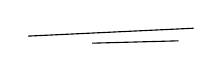
\begin{tikzpicture}\draw (0,0) -- (2.1,.10);\draw (.81,-.09) -- (1.91,-.06);\end{tikzpicture}}

\uline{Prop} Soit $G\xrightarrow{\deleted{\unsure{\lambda|v}}u}H$ \deleted{Si} hom de g.pes\deleted{, avec $G$ qu. cpt} Si $u$ est plat \inserted{(générisant)} en un p$^{\mathrm{t}}$, il est plat \deleted{(au \unsure{p. gén.})} \inserted{(\uline{univ} générisant)} \deleted{et \unsure{donc} \unsure{est} plat} ; \deleted{donc $u(G)$ stable par \deleted{spécialisation} générisat.}

% slanted
\margin{Il faut un argument pour ``univ'' générisant.}
\deleted{\uline{Cor} Supposons \deleted{que $H$ \unsure{qu cpt} qu'il existe} qu'il existe un p$^{\mathrm{t}}$ maximal $x$ de $H$ tel que $G_x\ne\varnothing$ (p. ex. $u$ dominant et $G$ qu. cpt) Alors \deleted{\unsure{$X$}} \inserted{si $H$ est réduit,} $u$ est plat, \deleted{donc généris\unsure{ant} (donc générisant \ldots)} Si on \inserted{ne} suppose pas \deleted{\uline{\unsure{Prop}} Su} avec $H$ réduit, $u$ est générisant, \deleted{et} l'image \deleted{\unsure{de}} $u(H)$ est stable \inserted{en} par générisation et \unsure{cont.|contient}}

\uline{Cor} Conditions équivalentes sur $u$

\deleted{\unsure{affine|ouvert}} a) $u$ est \inserted{univ} générisant \quad---\quad a$'$) $u$ générisant en un point.

b) $\unsure{U(G)|u(G)}\supset \deleted{G}H_0$

c) $\exists$ un point maximal \inserted{$x$} de $G$ tel que $u^{-1}(x)\ne\varnothing$.

Sous ces conditions, $u(G)$ est stable par spécialisation \deleted{(donc \unsure{fermé si} $G$ qu. cpt)}\margin{\deleted{\unsure{et H l. t. f.}}}

\uline{Dém} a) $\Longrightarrow$ a$'$) connu, a$'$) $\Longleftrightarrow$ b) \deleted{\illegible{1}} trivial, b) $\Longrightarrow$ c) trivial, prouvons c) $\longrightarrow$ b. Or $W=u(G)$ est stable \uline{par $\deleted{G}H_0$}, donc les $\varphi_x$ étant générisants, il est stable par spécialisation ; \deleted{OK} donc b) devient trivial.

% slanted
\margin{\deleted{avec} Est-il \uline{tjrs} vrai que $u(G)$ stable par spécialisation? Oui. Je prouve pour tt ss-ens. stable par mult (et sym.) $\to$ stable par spécia}
\uline{Cor} Si $G$ qu. cpt, \deleted{\unsure{domination} de $H^{\unsure{\mathrm{red}|\mathrm{t}}}$ \unsure{sur}} \inserted{$\operatorname{Im}u$ est fermée}

\uline{Prop.} Si $G\longrightarrow H$ un mono, avec $G$, \deleted{$H$} de t. f, \inserted{$H$ l. t. f.} alors $u$ est une immersion fermée.

\figure{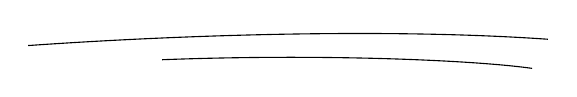
\begin{tikzpicture}\draw (0,0) .. controls (2,.14) and (4.6,.22) .. (6.6,.08);\draw (1.7,-.18) .. controls (3.8,-.10) and (5.7,-.19) .. (6.4,-.29);\end{tikzpicture}}

\diagram{$\displaystyle
\text{1)}\quad\left\{\begin{array}{l}
\text{Groupes discrets (ev. tordus)}\\
\text{Groupes profétales f. }(\text{---})\\
\text{Groupes loc. cpts (tot. discontinus) (ev. tordus}
\end{array}\right.
\quad\left|\begin{array}{l}
\text{groupes}\\
\text{séparables}\\
\text{tot. discontinus}
\end{array}\right.$}

\[
\begin{aligned}
\underline{\approx}\quad &\text{groupes topologiques loc. compact}\\
 &\text{\inserted{tot. disc.} avec opérations \uline{continues} de }\pi\\
 &\pi\times G\longrightarrow G\quad\text{continue.}
\end{aligned}
\]

\diagram{$\displaystyle
\text{2)}\quad\begin{array}{l|l}
\text{\uline{Groupes connexes}} & \text{\uline{sur corps parfait} : Extension (can.)}\\
\text{\uline{\deleted{\unsure{s|S}}Séparables}} & \text{d'une VA par un groupe connexe}\\
\text{[sont qu. cpts]} & \text{lisse affine}\quad\Longleftrightarrow\quad \underset{\longleftarrow}{\lim} G_i,\\
& \text{les }G_i\text{ de type fini, partie abélienne}\\
& \text{de dim. majorée.}
\end{array}$}
% archive sheet number: 5

\scanpage{7}
\deleted{$X$ \unsure{loc.} de type fini sur}

\uline{Prop} Soit $X$ schéma \deleted{\unsure{localement|loc. noeth}} \deleted{\unsure{noethérien}} \inserted{régulier} sur corps $k$ \deleted{\unsure{de}} \uline{parfait}. Soit $k'$ une extension de $k$, supposons que \deleted{les ann} $X$ soit loc. de t. f. sur $k$ ou $k'$ ext. de type fini de $k$, de sorte que les anneaux locaux de $X_{k'}$ sont noeth. Alors $X_{k'}$ est régulier

$\Updownarrow$\quad \uline{Corollaire} Soit $A$ un anneau local régulier sur $k$, $k'$ une extension de $k$. On suppose que $k'$ \deleted{est \unsure{loc.}} \inserted{ou $A$} de t. f. \deleted{\unsure{sur}} $k$., \deleted{\unsure{ou|{}} $A$ est de t. f. sur $k$} Alors $A\otimes_k k'$ est régulier.

% margin note written sideways
\margin{\uline{NB} Ne supposons pas $X$ \unsure{ess.|loc.} de t. f. sur $k$, \deleted{Il reste vrai que} \inserted{Alors si} $X$ est régulier pour tt extension \inserted{finie} \deleted{de la base} corps de base, \deleted{alors} pour tt $Y$ ess. de t. f. sur $S$, $Y$ régulier $\Longrightarrow X\times_kY$ \uline{régulier}. On dit que $X$ est géom régulier.}
% margin note written sideways
\margin{Ex : ext. de corps \uline{\unsure{alg.|sép.}}}
\uline{Prop} $X$ schéma \inserted{ess loc de t. f.} sur $k$, $k$, ext: parfait. Conditions équivalentes

\diagram{\begin{tikzcd}[ampersand replacement=\&,row sep=.75em,column sep=.8em,execute at end picture={\draw ([xshift=-.75em]\tikzcdmatrixname-1-1.north west) .. controls +(0,-.55) and +(.24,0) .. ([xshift=-1.2em]\tikzcdmatrixname-2-1.west) .. controls +(.24,0) and +(0,.55) .. ([xshift=-.75em]\tikzcdmatrixname-4-1.south west);}]
\text{a)}\arrow[d,Rightarrow] \& {\forall\ \text{schéma }Y\text{ sur }k,\ Y\text{ régulier}\Longrightarrow X\times_kY\text{ régulier}}\\
\text{b)}\arrow[d,Rightarrow]\arrow[dd,bend right=37,Rightarrow] \& {\forall\ \text{ext. }k'/k,\ X_{k'}\text{ est régulier}}\\
\text{c)} \& {\deleted{\forall}\,X_{\unsure{k,|k'}}\text{ régulier}}\\
\text{d)} \& {\forall\ \text{ext. finie }\deleted{\unsure{k'}}\ \text{radicielle }k'\text{ de }k,\ X_{k'}\text{ est régulier.}}
\end{tikzcd}}

\uline{Dém} b) $\to$ a) car si $A\to B$ hom$^{\mathrm t}$ local \inserted{plat} d'anneaux loc. noeth, $A$ régulier et $B/mB$ régulier \inserted{$\Rightarrow B$ régulier}

c) $\Rightarrow$ b) car si $\overset{\mathfrak m}{A}\to\overset{\mathfrak n}{B}$ hom local plat d'anneaux loc, noeth, \unsure{ds|des} $B$ régulier $\Rightarrow A$ régulier \ldots

d) $\Rightarrow$ c) par \unsure{principe} de limite.

\uline{Déf} On dit alors que $X$ est géom. régulier [ou \uline{lisse} sur $k$ si $X$ est loc. de t. f. sur $k$]

$X\deleted{\unsure{{}_k|{}_x}}$ \deleted{géom régulier}\deleted{lisse}\inserted{géom régulier} $\Longrightarrow X$ régulier. La réciproque est vraie pour tt $X$ sur $k$ (ou seulement pour tt $X=\operatorname{Spec}k'$, $k'$ ext. finie radicielle de $k$) ssi $k$ est parfait.

$X$, \deleted{géom rég}\deleted{lisse}\inserted{géom rég} $/k\Longleftrightarrow X_{k'}$ géom régulier sur $k'$

$X$ et $Y$ \deleted{géom réguliers}\deleted{lisse}\inserted{géom rég} sur $k$ $\Longrightarrow X\times_kY$ géom. réguliers sur $k$.

$X$ \deleted{\unsure{lisse}} géom. régulier/$k$ en \uline{un point} $x\in X$ : $\operatorname{Loc}_x(X)$ est géom rég sur $k$ \inserted{ou $\underline O_{X,x}$ est géom rég}

On a les faits analogues aux précédents.
\margin{\uline{NB} Si $k(x)$ est séparable sur $k$ régulier $\Rightarrow$ géom. rég.}

\deleted{\uline{Théorème} L'ens des p$^{\mathrm{ts}}$ de $X$, où $X$ est géom. régulier est ouvert. (On est ramené au cas où \deleted{\unsure{$X$}} $k$ est parfait \unsure{(i.e.|(} $=$ \unsure{Alg.|rég.} clos).)}

\uline{Prop}\inserted{(Critère jacobien)} $X$ \inserted{loc de t f sur $k$} est \deleted{géom régulier}\inserted{lisse} en $x\in X$ ssi il existe un \inserted{entier $n\geq0$ et} morphisme $f:U_u\longrightarrow\mathbb E^n_k$ ($U$ vois. ouvert de $x$) tel que $f$ soit ``étale'' en $x$, i.e. [loc. en prés. finie] plat et à fibres étales

\uline{Corollaire} L'ens des p$^{\mathrm{ts}}$ où $X$ est \deleted{géom} lisse sur $k$ est ouvert.
% archive sheet number: 6

\scanpage{8}

\uline{Corollaire.} Cet ouv est dense ssi pour \unsure{tt|tout} pt \uline{maximal} $x\in X$, $\underline O_{X,x}$ est réduit et $k(x)$ est une extension \uline{séparable} de $k$ $[\Leftrightarrow$ \inserted{\unsure{au cas une|au cas d'une} ext. de t. f.} extension étale d'une extension \unsure{transcend.te|transcendante|transcend. ou} pure$]$

\uline{Corollaire} Si $k$ est parfait, l'ens des pts où $X$ est lisse est un ouvert dense.

\uline{NB} On a un \unsure{réslt|rés\textsuperscript{t}} analogue pour la \uline{normalité géométrique}, sans condition de finitude. Si $X$ est \deleted{\unsure{géom normal|géom norm}} \inserted{loc de} t. f. sur $k$, l'ens des pts où $X$ est géom normal sur $k$ est ouvert, \inserted{et dense si $k$ est parfait} [Une extension d'un corps est géom normale ssi elle est séparable)

\figure{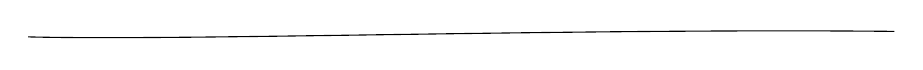
\begin{tikzpicture}\draw (0,0) .. controls (2,-.05) and (7,.11) .. (11,.07);\end{tikzpicture}}

\uline{Proposition} $G$ groupe sur corps $k$. Conditions équivalentes

\margin{marche aussi si $X$ un \deleted{\unsure{gpe|esp.}} \inserted{schéma} sur lequel $G$ opère et tel que \deleted{$G\times X\xrightarrow{\unsure{\pi|p}} X$} $G\times X\longrightarrow X\times X$ surjectif $(g,x)\longmapsto(gx,x)$ ($X$ essentiellement homogène)}% slanted

a) $G$ \deleted{\unsure{géom norm|géom. normal}} séparable $/k$ en un pt \qquad a$'$) $G$ sép. $/k$ \deleted{en un point}

b) $G$ géom normal sur $k$

c) (Si $G$ loc de t. f. sur $k$) $G$ lisse $/k$

On a évidemment \inserted{c $\Rightarrow$} b) $\Rightarrow$ a$'$) $\Longrightarrow$ a) \deleted{$\Longrightarrow$ \unsure{b)|b)?}}.

\margin{\uline{NB} Si $G$ de t. f. sur $k$, alors $G$ \deleted{\unsure{re|ré}} \unsure{réduit|reduit} $\Rightarrow G$ sép.? \deleted{(\unsure{est-ce que|et si pas|est-ce} le \unsure{$k$|$h$} \unsure{est} \unsure{stable dans|étant donné}}}% slanted

a) $\Rightarrow$ b) \qquad Soit $g\in G$, \deleted{un} pt maximal de $G$. \deleted{\unsure{géom|gén.}} \deleted{pour que $g$ \unsure{$G$ est géom normal en $g$|soit géom il suffit que $g$},} Alors $k(g)$ est une ext. séparable de $k$, donc $G$ est géom normal en $g$. \deleted{Donc, quitte \unsure{à faire une extension|à une extension} par descente on est ramené à \unsure{voir le cas|voir l'assert} pour $g$ rat. sur $k$.} \deleted{Soit $g'$ un pt maximal de $G$, on sait que $G$ est géom normal en $g'$; faisant une extension} Donc $G$ a \uline{un} pt $g$ où il est géom. normal. Prouvons qu'il en est de $=$ pour tt autre pt $g'$. Par ext. de la base, on est ramené au cas où $g$, $g'$ rat $/k$. Mais alors ils sont conjugués par translation !

b) $\Rightarrow$ a) \qquad \unsure{Esq.|Est.} en démonstration.

\uline{Corollaire 1} Soit $k$ parfait. Alors $G_{\text{\unsure{red|réd}}}$ est géom normal \unsure{$\bar k$|$k$|$\bar B$} (resp. lisse, si $G$ est loc. de t. f. sur $k$)

% archive sheet number: 7

\cotefile{53}
\scanpage{9}
% slanted
\margin{C'est \unsure{faux|sans|sous}} \deleted{\unsure{Coroll.|Coroll 1}} \uline{Corollaire} 2 \deleted{\unsure{Toute|Toutes}} \inserted{Les} \uline{composantes irréductibles de $G$} \deleted{(supposé loc. de t. f.)} \uline{sont les composantes connexes}. \uline{En particulier}, $G^{\unsure{0|\circ}}$ \uline{est irréductible}.

On peut supposer $k$ parfait, $G$ réduit donc normal (resp. lisse). Mais alors c'est \uline{vrai pour tt schéma normal} \inserted{(lisse)} sur $k$.... On a supposé ici $G$ loc. de t. f. sur $k$. Sinon on peut dire que $G_0$, la comp. irréd. de \unsure{$e$|$k$}, est stable par générisation, donc contient $\operatorname{Loc}_e(G)$.

% slanted
\margin{\textcircled{?} \deleted{C'est dans} le cas loc. de t. f. au moins}

% slanted
\margin{$-$ \unsure{$W^{\mathrm{no}}$|$W^{\mathrm{ro}}$|$N^{\mathrm{ro}}$} en $G$ \uline{loc. de t. f.}}

\deleted{\uline{Corollaire} 3 Pour \deleted{deux} ouverts $U$\inserted{, $V$} de $G$, \inserted{\deleted{loc. de t. f.} On peut s'en \inserted{dispenser} \deleted{supposer} $U$ \deleted{et} $V$ qu. cpct \uline{ou} $G$ loc. de t. f.)} $U\deleted{\unsure{U'|U}}V$ \deleted{contient $G^0$, si $U,U'$ sont des ouverts de $G$ qui contiennent $e$, $UV\supset G^0$.} \inserted{est une partie à la fois ouverte et fermée de $G$ (\unsure{évidemment|évidemt|évident} qu. cpct)}, donc stable par translation par $G^0$.}

\deleted{\deleted{\unsure{La deuxième assertion|La deuxième étant} conséquence immédiate de 2} première \deleted{\unsure{on le|on la} \unsure{pour|peut}} l'appliquant : $W=U\cap U^{-1}\cap V\cap V^{-1}$. \deleted{\illegible{2}} Pour prouver $UU^{-1}\supset G^0$, \deleted{\unsure{on peut}} \inserted{OPS par descente que $U$ contient pt rat $/k$, et par translation que $U\ni e$.} Soit $g\in G^0$, il faut montrer que (sur une ext $k'$ de \unsure{$k(g)$|$\kappa(g)$}) $g=\deleted{\unsure{g|g'}}uv^{-1}$, avec $u,v\in U(k')$, i.e. $(gU\cap U)(k')\ne \unsure{\phi|\varnothing}$, \deleted{et il suffit de prouver que (sur $k_1=k(g)$)} \deleted{$\unsure{gU\cap U\ne\varnothing|gU\cap U\ne e}$} or $gU\cap G^0$ et $U\cap G^0$ sont des ouverts non vides de $G^0$ (contient $g$ et $e$, donc ont une intersection non vide, puisque $G^0$ est irréd.}

\deleted{\uline{Autre dém} $G\times G \unsure{-|\longrightarrow} G$ est plat (car isom à $G\times G\xrightarrow{\mathrm{pr}_{1}}G$) de \deleted{\unsure{ses|sa}} générisant, donc l'image de $U\times U$ est stable par générisation, donc si $G$ est loc. de t. f.}

\deleted{La $=$ démonstration montre que $U.V$ stable par translation par $G^0$, donc étant qu. cpct il est \deleted{stable} ouvert et fermé.}

\deleted{$U.V$ ouvert comme image de $U\times_k V\subset G\times_k G$ par $G\times_k G \unsure{-|\longrightarrow} G$, qui est ouvert (isom : $G\times G\underset{\mathrm{pr}_1}{-}G$ qui l'est).}

\deleted{D'autre part, pour prouver que $U.V$ est fermé, il suffit, comme $U.V$ est \deleted{\unsure{vide ou quasi|vide ou qu. cpct}} qu. cpt donc rétrocompact (dans $G$ \uline{séparé}), \deleted{pour} de voir que $x\in U.V$, \deleted{$\unsure{\Rightarrow x\in U.V.|\Rightarrow y\in U.V.}$} \inserted{$y\in \unsure{(x)|\overline{(x)}|\overline{\{x\}}}$, alors $y\in U.V$.} On est ramené à \deleted{prouver} le prouver pour $x$}

% archive sheet number: 8

\scanpage{10}
Rectificatif sur critère d'irréductibilité géom.

\diagram{\begin{tikzcd}[ampersand replacement=\&,column sep=1.6em,row sep=.45em]
{} \&[-.3em] {} \&[-.5em] Z'\arrow[dr,dash,"{f'}"'] \& {}\\
Z\arrow[r,"f"] \& X\arrow[d,dash] \& {} \& X'\arrow[ll,"p"']\arrow[d,dash]\\
{} \& k\arrow[rr,dash] \& {} \& k'\\
{} \& {} \& {} \& \deleted{\text{sép clos}}
\end{tikzcd}}
Supposons a) $Z$ géom. irréd, b) $f(Z)$ non contenu dans l'ens des points \deleted{\illegible{1}} où passent plusieurs comp. irréd. géom (p. ex. $f(Z)$ contient un pt géom normal, \deleted{\unsure{ou|un}} \inserted{voire} géom régulier, de $X_{\mathrm{red}}$). Alors $X$ géom irréductible.

\uline{Dém} [OPS $Z$ réduit à un pt \deleted{de} $x$ de $X$.] \deleted{\unsure{Puis $X$ irréd|Alors $X$ irréd|On a $X$ irréd|Alors $X$ étant}} Soit $k'$ \deleted{clôture séparable} \inserted{ext finie gal.} de $k$, \deleted{Alors} $X'_i$ une composante irréductible de $X'$.  \deleted{Elle domine} contenant $f'(Z')$\inserted{(qui est irréd)}, les \unsure{transformés|transformées} par $\pi$ sont des composantes irréductibles contenant $f'(Z')$, donc sont \uline{égales} à $\deleted{\unsure{f(|g(}}X'_i$.  Donc $X'_i$ est l'image inverse de une partie fermée irréductible de $X$, savoir de $\unsure{p|p'|f}(X'_i)$, or $p(X'_i)=X$ [platitude \deleted{\unsure{de|du}} ] $p$ + $p$ fermé], donc $X'_i=X'$, donc $X'$ est irréd.

Contr'exemple si on laisse tomber b)

\[
X=\mathbb{R}[x,y]/(x^{\unsure{7|2}}+y^2),\quad Z=\operatorname{Spec}\mathbb{R},
\]
\diagram{\begin{tikzcd}[ampersand replacement=\&,row sep=.2em,column sep=1.5em]
Z\arrow[r] \& X\\
\mathbb{R} \& \mathbb{R}[x,y]/{-}\arrow[l]\\
0 \& x,y\arrow[l,maps to]
\end{tikzcd}}
\par\noindent\hfill\rule{.25\linewidth}{.4pt}\hfill\strut\par
\deleted{Complément sur $\pi_0(X/k)$}

\uline{Remarque} Dans l'équivalence $\mathrm{Et}(k)\simeq(\pi\text{-}\mathrm{Ens})$, \deleted{les ensembles} \deleted{\unsure{on voit|on a vu}} \margin{\deleted{$\unsure{k'\underset{\pi}{\longleftarrow}k|k'\underset{\pi}{-}k'}$}}

\diagram{\begingroup\small\(\left\{\begin{array}{@{}l@{\;\;}l@{}}
\multicolumn{1}{c}{X} & \multicolumn{1}{c}{E}\\
\parbox[t]{.43\linewidth}{$X$ quasi-compact (de degré $n$)} & \parbox[t]{.44\linewidth}{--- $E$ fini (dé ordre $n$)}\\[.5ex]
\parbox[t]{.43\linewidth}{\deleted{Décomposition de $X$ en}} & {}\\
\parbox[t]{.43\linewidth}{$X$ connexe [ou : irréductible], \inserted{ou $X\simeq\operatorname{Spec}K$, $K$ ext. finie sép.]}} & \parbox[t]{.44\linewidth}{--- $\pi$ transitif sur $E$}\\[.6ex]
\parbox[t]{.43\linewidth}{Décomposition de $X$ en somme de compos. \deleted{\unsure{disjointes|disj.}} connexes $\ne$} & \parbox[t]{.44\linewidth}{--- décomposition de $E$ en sommes d'orbites}\\[.6ex]
\parbox[t]{.43\linewidth}{$\varprojlim$ finies de schémas} & \parbox[t]{.44\linewidth}{--- $\varprojlim$ finies de $\pi$-ens}\\
\parbox[t]{.43\linewidth}{$\varinjlim$ \deleted{\unsure{fin|finies}} de schémas.} & \parbox[t]{.44\linewidth}{--- $\varinjlim$ de $\pi$-ens.}\\
\parbox[t]{.43\linewidth}{mono $X\to Y$ \inserted{(resp. épi)}} & \parbox[t]{.44\linewidth}{--- $\unsure{E-F|E\to F}$ injectif (resp. surjectif)}\\
\parbox[t]{.43\linewidth}{[$X$ un torseur \inserted{à dr.} sous $G$ \deleted{groupe f} groupe fini ordinaire} & \parbox[t]{.44\linewidth}{$E$ un torseur à droite sous $G$; les opérations de $G$ commutant à l'action de $\pi$ (donc si on choisit un $e\in E$, la structure est définie par un hom continu $\pi\to G$)]}
\end{array}\right.\)\endgroup}
\uline{Rappel sur la construction de} $\pi_0(X/k)$ lorsque \deleted{\unsure{pour les extensions|pour des extensions}} \deleted{\unsure{génér.|pour}} $X_{k'}$ ($k'$ clôture parfaite de $k$) est localement connexe, \deleted{\unsure{donc|dans}} \inserted{et} les \deleted{\unsure{$X_{k'}$|$X_k$}} composantes connexes définissables sur des \inserted{\unsure{ss.|sép.|sé.}} ext. finies de $k$ (p. ex. $X$ qu. cpct, ou $X$ loc. de \uline{\unsure{pr. finie|p. finie|t. f.|t. fini}} sur $k$)

\mspage{2}
% archive sheet number: 9

\scanpage{11}
\deleted{\illegible{1}} Les pts \inserted{$x$} de $\underline{\pi_0}(X/k)$ correspondent aux \uline{composantes} \uline{connexes} de $X$, pour toute telle composante $X_{(x)}$, $k(x)$ est la plus grande sous-algèbre entière séparable de $\Gamma(X_{(x)},\underline{O}_{X_{(x)}})$ sur $k(x)$.

Que se passe-t-il pour $X=\operatorname{Spec}k'$ ? \deleted{\unsure{de|du}}

On a $k'=\varinjlim k_i$,\inserted{(\unsure{sous-ext.|sous-cat.} \unsure{galoisiennes|galoisienne} \unsure{finies|finie} de $k'$)} $\Rightarrow X=\varprojlim X_i$, $X_i=\operatorname{Spec} k_i$.

\[
\begin{aligned}
X'&=\varprojlim X'_i=\varprojlim_i(\pi_i)_{k}=(\pi)_k\\
\pi_0(X')&=\pi\quad(\text{isom. \uline{topologique}})
\end{aligned}
\]
\deleted{Ce n'est plus un schéma étale sur $k$}

Schéma proétale sur $k$ [\deleted{compact, réduit, à corps résiduels} \inserted{$=$ entier séparable $=$} \deleted{\unsure{à points ext.|à points isolés}} réduit à ext. résiduelles \deleted{\unsure{étal|étal.}} alg. sép.]

\deleted{\S} [Schéma loc. proétale sur $k$]

\[
\left\{\begin{aligned}
\mathrm{ProEt}(k)&\cong\pi\text{-esp cpt tdisc.}\cong\mathrm{Alg}_{\text{\unsure{indét|indet|ind-et}}}(k)\\
\mathrm{Locproet}(k)&\cong\pi\text{-esp loc. cpt disc.}
\end{aligned}\right.
\]
Si $X$ qu. cpct sur $k$ (pour simplifier) on construit une algèbre \unsure{indétale|proétale} \deleted{sur $X$} $k$, au choix

a)

\[
\begin{aligned}
A&=\text{limite inductive des sous-}\underline{\unsure{\mathrm{Alg}^{\prime\prime}\mathrm{bres}|\mathrm{Al}''\mathrm{bres}}}\ \text{étales de }\Gamma(X,\underline{O}_X)\\
&=\text{\deleted{limite} plus grande sous-Alg. ind-étale de }\Gamma(X,\underline{O}_X).\\
X&\longrightarrow\operatorname{Spec}(A)\overset{\text{dfn}}{=}\underline{\pi}_0(X/k)
\end{aligned}
\]
b) Pour toute ext. \deleted{finie} \inserted{étale} $k_i\subset k'$ de $k$, on désigne par \deleted{\unsure{$k$|$A$}} $A_i$ l'anneau des fonctions loc. constantes sur $X_{k_i}$, à valeurs dans $k_i$. Soit $\overline A=\varinjlim_i {A_i}_{k'}$, \inserted{fonctions loc. constantes sur $X_{k_i}$ \unsure{à v.|à val} dans $k'$} \deleted{\unsure{alors|ainsi} $\pi$ opère} \inserted{fonctions} loc. constantes sur $X_{k'}$ à valeurs dans $k'$, Alors \inserted{$\overline A$ est ind-étale et} $\pi$ opère dessus par transfert des structures, on pose $\overset{\deleted{\unsure{\text{donc}|\text{alors}}}}{A}=(\overline A)^\pi$.

\par\noindent\rule{.20\linewidth}{.4pt}\par
\[
\left\{\begin{array}{ll}
\text{a)} & \parbox[t]{.82\linewidth}{$\deleted{X\to}\underline{\pi}_0(X/k)$ est proétale et $X\to\underline{\pi}_0(X/k)$ \deleted{est} surj. à fibres géom. connexes}\\[.7ex]
\text{b)} & \underline{\pi}_0(X/k)\ \text{fonctoriel en }X\\[.7ex]
\text{c)} & \underline{\pi}_0(X/k)\ \text{commute au produit}\\[.7ex]
\text{d)} & \underline{\pi}_0(X/k)\ \text{commute à l'extension de la base ....}
\end{array}\right.
\]
\uline{NB} $\underline{\pi}_0(X/k)$ peut se définir comme schém. loc proétale, \deleted{si} toute pt de \deleted{ce} $X$ a un voisinage ouvert et fermé $U$, tel que \deleted{\unsure{la|le}} la décomposition de $U_{k'}$ en somme \deleted{\unsure{de|s}} \deleted{soit} soit finie (p. ex. $U$ qu. cpct).

% archive sheet number: 10

\scanpage{12}
\uline{Schémas sur un corps.}

\deleted{\uline{Rappels} \textcircled{\unsure{1|2}} \unsure{Lorsque|Lorsque le} $k$ est parfait, \unsure{réduites.|réduite.}}

\margin{\textcircled{1} \uline{Séparabilité}}

% slanted
\uline{Rappel} Soit $k$ un corps. Conditions équivalentes

\[
\left\{\begin{array}{ll}
\text{a)}&\parbox[t]{.80\linewidth}{$k$ parfait i.e. $k$ de car. $0$, ou (si car $p\unsure{>|\ne}0$) $x\mapsto x^p$ est bijectif)}\\
\text{b)}&\text{un produit tensoriel d'algèbres réduites sur }k\text{ est}\\
\text{b')}&\Rightarrow\ \text{Un produit sur }k\text{ de schémas réduits est \inserted{réduit}}\\
\text{c)}&\parbox[t]{.80\linewidth}{Pour tt extension finie $k'$ de $k$, \inserted{(\unsure{radicielle|\deleted{qu}radicielle} de degré $p$ si on veut)} \deleted{\unsure{on|un}} $k' \otimes_k k'$ est réduit}
\end{array}\right.
\]
Soit $A$ une algèbre sur un corps $k$, \inserted{$k_1$ une extension parfaite de $k$,} Propriétés équivalentes

\inserted{a) $\forall$ $k$ algèbre réduite $B$, $A\otimes_k B$ réduit}

b) $\forall$ extension $k'$ de $k$, $A\otimes_k k'$ réduit

c) $A\otimes_k k_1$ est réduit

d) $\forall$ ext. finie \deleted{\unsure{sép.|sép}} radicielle de $k$, $A\otimes_k k'$ est réduit.

\margin{faire passage \unsure{à la|à l'} limite pour prouver que $A\otimes_k k^{\unsure{\mathrm{pf}|\mathrm{perf}|p}}$ est réduit}

% slanted
\uline{Déf} On dit alors que $A$ est \uline{séparable} sur $k$ (ou \uline{géom.} \uline{réduit})

\uline{Cor} Soit $X$ schéma sur $k$. Propriétés équiv.

a) \deleted{\unsure{Pour tout|Pour tout un}} tout \inserted{$k$-}schéma réduit $Y$, $X\times_k Y$ réduit

b) Pour tte \deleted{corps} extension $k'$ de $k$, $X_{k'}$ réduit

c) $X_{k_1}$ est réduit

\margin{\deleted{Cor}} d) (Si $X=\bigcup X_i$, les $X_i$ affines \deleted{\unsure{$\exists$|$A$}} d'anneaux $A_i$) les $A_i$ sont séparables $/k$

\uline{Déf} On dit alors que $X$ est sép. sur $k$, ou encore \deleted{\unsure{géo|géom.}} \inserted{géom.} réduit.

Ainsi, \deleted{$k$ est parfait ssi} tt schém. \inserted{géom.} réduit sur $k$ est \deleted{\unsure{géom.|géo}} réduit, la réciproque étant vraie \unsure{ssi|si} $k$ est parfait

\uline{NB} Si $k'/k$ est une extension de $k$, $X_{\deleted{\unsure{f|k'|k}}}$ sép. sur $k$ $\Longleftrightarrow X_{k'}$ sép $/k'$

C'est un critère ``géométrique''. \hfill\uline{Stabilité par produit}

\margin{\textcircled{2} \deleted{\uline{Intégrité}} \uline{Irréductibilité}}

% slanted
\uline{Rappel} Soit $k$ \deleted{séparable}, corps. Conditions équivalentes

a) $k$ sép. clos i.e. \deleted{\unsure{toute|tout}} ext. finie séparable de $k$ est $\simeq k$

b) Si $A$ et $B$ sont deux $k$-\deleted{\unsure{schémas irréductibles|schémas intègres}} \inserted{algèbres intègres}, $A\otimes B/\mathrm{\unsure{Nil|N.il}}$ est intègre

[b') Si $X,Y$ sont deux \inserted{$k$-}schémas irréd, alors $X\times_k Y$ est irréd]

c) Si \deleted{\unsure{$k'$|$k$}}, $k'$ est une extension finie de $k$, $k'\otimes_k k'\longrightarrow\deleted{\unsure{k|k'}}k'$ a un noyau nilpotent

\margin{Toute $\varprojlim$ filtrante d'espaces top. sobres irréd (resp. connexes) est irréd (resp. connexe)}

% slanted
Soit $X$ schém. sur corps, $k_1$ une extension sép. close de $k$ \uline{Conditions} équivalentes

a) $\forall Y$ sur $k$, $Y$ irréductible, $X\times_k Y$ est irréductible

b) $\forall$ extension $k'$ de $k$, $X_{k'}$ est irréductible

c) $X_{k_1}$ est irréductible

d) p. tte ext. finie \deleted{gal.} $k'$ de $k$, $X\otimes_k k'$ irréd.

\margin{faire passage à la limite ($\varprojlim$ d'irréd. par des morphismes dominants est irréd)}

% slanted
% archive sheet number: 11

\scanpage{13}
\uline{Déf} On dit alors que $X$ est géom. irréductible.

Ainsi \deleted{$k$ est sép. clos ssi} tout \inserted{$k$-}schéma irréductible est géom. irréductible, réciproque vraie ssi $k$ est sép. clos.

\uline{NB} Si $k'/k$ une extension, $X_k/k$ géom irréd $\Longleftrightarrow X_{k'}/k'$ géom irréd. \margin{$\big/$\,Stabilité par produit}

\margin{\textcircled{3}} \deleted{\uline{\unsure{Remarque|Réciproque}}}

\noindent\vrule width .55pt\hspace{.5em}\begin{minipage}{.92\linewidth}
\uline{Th} Soit $k$ un corps sép. clos. Si $X$ et $Y$ sont deux $k$-schémas connexes, $X\times_k Y$ est connexe.

\end{minipage}\par
\uline{Dém.} dans le cas où $X$ et $Y$ sont loc. de \unsure{v.|t.} f. sur $k$. (Cas général utilise technique de descente\}, plus précisément que $X\times Y\longrightarrow Y$ la top. de $Y$ est quotient de celle de $X\times Y$.

a) Si $X$ est connexe \inserted{non vide}, $X_{k'}$ est connexe \inserted{non vide}, pour tte extension $k'$ de $k$ [en effet, les fibres de $X_{k'}-X$ sont connexes \inserted{non vides}]

b) les fibres de $X\times Y\to Y$ étant connexes \inserted{non vides} et $Y$ connexe, $X\times Y$ est connexe

\uline{NB} Si $k$ est un corps tel que pour tt $X$ \inserted{connexe,} fini sur $k$, $X\unsure{\otimes|\times}_k \unsure{\alpha|X|x}$ est connexe alors $k$ est sép clos.

\uline{Prop} Soit $k$ un corps, $k_1$ une ext. \deleted{alg} sép. close, $X$ un $k$-schéma. Conditions équivalentes

a) $\forall$ $k$-schéma $Y$, $X\times_k Y$ est connexe

b) $\forall$ \unsure{ext.|lxt.} $k'$ de $k$, $X_{k'}$ est connexe

c) \deleted{$\unsure{\forall|\forall k}$} $X_{k_1}$ est connexe.

d) $\forall$ ext. finie \unsure{\deleted{gal.}|gal.} $k'$ de $k$, $X_{k'}$ est connexe.

\margin{passage à la limite, prenant $k_1=$ clôture sép en $k$, et en utilisant que $\operatorname{Spec} k_1 -\operatorname{Spec} k_i$ est univ. ouvert.}

% slanted
\uline{Déf.} On dit alors que $X$ est \uline{géom. connexe} sur $k$.

Ainsi \deleted{\unsure{le corps|connexe|connexe ssi}} \inserted{géom} connexe sur $k$ $\Rightarrow$ connexe, la réciproque vraie ssi $k$ est sép. clos.

\uline{NB} $X_k$ géom connexe $/k$ $\unsure{\Longleftrightarrow|\Longrightarrow} X_{k'}$ géom. connexe sur $k'$.

Stabilité par produit.

\margin{\textcircled{4} \uline{intégrité}}

% slanted
$k$ un corps. Conditions équivalentes

\deleted{a) Si $X$ et $Y$ deux $k$-algèbres intègres}

a) $k$ alg clos

b) Si $A,B$ sont deux $k$-algèbres intègres, $A\otimes_k B$ intègre

b') \deleted{\unsure{Soit|Si les|Si}} $X,Y$ intègres $\Rightarrow X\times_k Y$ int.

c) Pour tte ext. finie $k'$ de $k$, $k'\otimes_k k'$ intègre.

% archive sheet number: 12

\scanpage{14}
\uline{Prop} Soit $X$ un schéma sur corps $k$, $k_1$ une ext. alg. close de $k$. Cond. équiv.

a) $\unsure{\forall|\deleted{V}\forall}$ $k$-schéma intègre $Y$, $X\times_k Y$ intègre.

b) $\forall$ \unsure{ext.|lxt.} $k'$ de $k$, $X_{k'}$ intègre

c) \deleted{$\unsure{\forall|\forall k}$} $X_{k_1}$ intègre

\uline{Déf} On dit alors que $X$ est géom intègre ($\Longleftrightarrow$ géom irréd et géom réduit)

Ainsi géom intègre $\Rightarrow$ intègre, réciproque vraie ssi $k$ alg clos.

$X_k/k$ géom int. $\Longleftrightarrow X_{k'}/k'$ géom. intègre

Stabilité par produits

\par\noindent\rule{.22\linewidth}{.4pt}\par
\uline{Prop} Soit $X$ sur corps $k$, $Z\xrightarrow{u}X$, $X$ connexe \inserted{\deleted{(irréductible)}}, $Z$ géom. connexe \inserted{non vide \deleted{(resp. géom irréd)}}, (p. ex \inserted{non vide} radiciel$/k$).

\noindent\vrule\enspace Alors $X$ est \deleted{\unsure{géom.|géomt}} connexe \deleted{(géom irréd)}.

Soit $k'$ \deleted{la clôture sép. de $X$.} \inserted{extension finie galoisienne}. Alors $\Pi=\operatorname{Gal}(k'/k)$ opère sur $X_{k'}=X\times_k\operatorname{Spec}(\unsure{k'|k'_i})$ et sur $Z_{k'}$, de façon à commuter à $u_{k'}: Z_{k'} - X_{k'}$.

\deleted{Les} \inserted{Soit $U$} parties ouvertes et fermées de $X_{k'}$, \deleted{\unsure{si il est|s'il est}} \inserted{prouvons qu'elle} \deleted{\unsure{qu'on, considérons|est $\varnothing$, considérons}} \inserted{est $\varnothing$ ou $X_k$} prouvons qu'elle est stable sous l'action de $\Pi$. En effet,

\deleted{\unsure{Si|Soit} $g\in$ $U$ contient} Quitte à rempl. $U$ par $\complement U$, on peut supposer que $U$ contient $u_{k'}(Z_{k'})$, qui est stable par $\Pi$, donc l'intersection \inserted{\unsure{$\forall$|de|$\pi$}} des

\deleted{ouverts fermés qui contiennent $u_{k_1}(Z_{k'})$ est \deleted{\unsure{bien|un}} stable sous $\Pi$,} \unsure{transformés,|transformés} de $U$ par les $g\in \unsure{\Pi|\mathrm{G}}$ est un ouvert stable \deleted{tel que} : \deleted{donc c'est l'image inverse d'une partie de $X$} non vide, provenant donc d'un ouvert \deleted{\unsure{et fermé|stable de}} de $X$, etc

\par\noindent\rule{.94\linewidth}{.4pt}\par
\uline{Ex} Composante neutre \inserted{$G^{\unsure{0|\circ}}$} d'un groupe algébrique \deleted{[elle est quasi-compacte} [Quand elle est ouverte, p. ex. $G$ loc. de t. f. sur $S$, alors on la munit de la structure induite]

$G_{\mathrm{red}}$ pour $k$ \uline{parfait} : un sous-groupe fermé de $G$

$G^{0}_{\mathrm{red}}$ id

[Soit $U$ \deleted{\unsure{et|deux}} \inserted{$\unsure{\varnothing|V}$} ouverts de $G$ ; alors $U.\unsure{U|V}^{-1}\supset G^0$ [\,$\Rightarrow$ et si $U,V$ \unsure{contient|contiennent} l'\unsure{élémt|élément} neutre, $UV\supset G^0$] [Cor. $G^0$ quasi-compact.]

% archive sheet number: 13

\scanpage{15}
Schémas (finis) étales sur un corps $k$ : la catégorie est équivalente : la catégorie des $\pi$-ensembles (finis), $\pi=\operatorname{Gal}(\bar k/k)$.

\uline{Application} Soit $X$ un schém. sur $k$, Supposons d'abord que $X_{\bar k}$ est loc. connexe [p. ex. loc. noeth, ou ens des composantes irréductibles loc. fini ; \unsure{tout est ok|tout est OK} si $X$ est loc. de t.f. sur $k$]. Alors $I=\pi_0(X_{\bar k})$ est un ens. discret, et on a un \deleted{\unsure{$\varphi$|f}} morphisme de $\bar k$-schémas

\diagram{\begin{tikzcd}[ampersand replacement=\&]
X_{\bar k}\arrow[d]\\
I_{\bar k}
\end{tikzcd}}
(il est universel pour les morphismes de $X$ dans des schémas constants). D'ailleurs $\pi$ opère sur $\deleted{I_{\bar k}} I$, donc $I_{\bar k}$ provient d'un \deleted{$I$} \unsure{sur|\deleted{sur}} schém. étale $T$ sur $k$ [si on prouve que $\pi$ opère continûment -- ce sera le cas en tous cas si $X$ est quasi-compact].

\margin{i.e \deleted{tte} composante connexe de $X_{\bar k}$ est \unsure{déjà|déja} définie sur une \inserted{\unsure{ss-|s.-|sép.}}ext. finie de $k$. \uline{C'est vrai} \uline{si} $X$ \uline{qu. cpct}, \deleted{\unsure{mais|aussi}} \deleted{\illegible{2}}}

% slanted
Alors la théorie de la descente nous prouve que $X\simeq X_{\bar k}/\pi$, $T=I_{\bar k}/\pi$, (dans catégorie des schémas) donc on trouve

\diagram{\begin{tikzcd}[ampersand replacement=\&]
X\arrow[d,"f"]\\
T
\end{tikzcd}}
$T$ étant étale sur $k$, \deleted{et} On \unsure{a|â|à} que $f$ est surjectif et à fibres géom connexes -- et ceci suffit à caractériser $X$. On peut aussi décrire comme le morphisme universel de $X$ dans un schém. étale sur $k$.

\margin{$T$ est appelé le schém. des composantes connexes géom. de $X$. Un pt à val. dans un $S'/k$ ``est'' une partie ouverte et fermée de $X_{\unsure{\xi|S'|S}}$, \unsure{/|,} qui \unsure{est|\deleted{est}}}

\diagram{\begin{tikzcd}[ampersand replacement=\&,column sep=large]
X\arrow[d] \& X'\arrow[d,dash]\\
T\arrow[d] \& T'\arrow[d,dash]\\
S=\operatorname{Sp} k\arrow[r,dash] \& S'
\end{tikzcd}}
\uline{Généralisation} On suppose $X$ quasi-compact, ou somme de schémas quasi cpcts : On trouve un $T$ \inserted{affine} pro étale, ayant les \unsure{\={m}s|\~{m}s} propriétés$\scriptscriptstyle\wedge$ qu'avant. Le foncteur qu'il représente est un peu plus subtil à décrire....

% archive sheet number: 14

\cotefile{53}
\scanpage{16}
\[
\left\{\begin{aligned}
&\text{Groupes sur des bases } S\ \text{quelconques. Prendre base } S\ \deleted{\unsure{?}}\ \text{ou prendre base } k\ \text{?}\\
&\text{Groupes n.-affines O.K.}
\end{aligned}\right.
\]

Représentations linéaires des $D(M)$ [cas particuliers : $\mathbb{G}_m$, $\mu_n$]

Application : homomorphismes $D(M)\longrightarrow\mathbb{G}_m$ : on trouve que $M_S$ est ``réflexif'' vis à vis de $\mathbb{G}_m$.

\uline{Dualité de Cartier}\quad $\underline{\mathrm{Hom}}_{\mathrm{gr}}(G,\mathbb{G}_m)$ \deleted{\unsure{$\overset{\Delta}{=}$|est}} représentable ? Cela l'est si $G$ diagonalisable, mais \deleted{pas}\inserted{en général (= pour $G=\mathbb{G}_m$)} pour un schéma en groupes affine (même de t.f.). Par contre, si $G$ est fini loc. libre sur $S$, on a
% slanted
\reversemarginpar\margin{$\underline{\mathrm{Hom}}_{\mathrm{gr}}(G,H)$ représentable si $G$ est fini loc. libre, et $H$ affine (disons)}\normalmarginpar
\[
\underline{\mathrm{Hom}}_{\mathrm{gr}}(G,\mathbb{G}_m)
\subset \mathrm{Hom}_{\unsure{\mathcal O|O|\mathbb O}\text{-alg}}
(\mathcal O_S[T,T^{-1}],\mathcal A)\simeq W(\mathcal A)^*,
\]
et le sous foncteur est celui des \deleted{$g$} $u\in W(\mathcal A)^*(S')$ tels que
\[
\Pi(u)=u\otimes u\qquad \varepsilon(u)=1
\]
\margin{[\,\uline{NB} On peut donc oublier la condition $u$ inv. car $\underline{\mathrm{Hom}}_{\mathrm{gr}}(G,\mathbb{G}_m)=\underline{\mathrm{Hom}}_{\mathrm{mon}}(G,\mathcal O^{\times})$.}

\deleted{La} La représentabilité est claire, mais de plus on reconnaît que c'est \deleted{\unsure{le|à}} $\mathrm{Spec}(\check{\mathcal A})$, $\check{\mathcal A}$ \deleted{étant}\inserted{$=\underline{\mathrm{Dist}}(G)_{S}$} une algèbre grâce à la structure de coalgèbre de $\mathcal A$. D'autre part, la structure de coalgèbre de $\check{\mathcal A}$ (provenant du fait que le foncteur qu'il représente est un foncteur-groupe
% slanted
\reversemarginpar\margin{$\check{\mathcal A}$ comm. car $G$ l'est. Si $G$ n'est pas comm., il faut prendre le foncteur $k'\longmapsto\mathrm{Hom}_{k\text{-alg}}(\check{\mathcal A},k')=\mathrm{Hom}_{k\text{-alg}}({\check{\mathcal A}\deleted{\unsure{)}}}_{\mathrm{ab}},k')$}\normalmarginpar

\uline{Th.} Tout groupe comm. fini loc. libre \inserted{$G$} est réflexif pour
\par\noindent\begin{tabular}{@{}|p{.91\linewidth}@{}}
$\mathbb{G}_m$. Son dual $G^*$ est fini loc. libre comm., d'où une \uline{\unsure{d'involution|involution}} $G\unsure{\mathrel{\vert\!-\!{\cdot}}|\mapsto}G^*$ de la catégorie des groupes comm. loc. libres. Elle correspond à la dualité des bialgèbres bicommutatives sur $S$.
\end{tabular}

\[
\begin{aligned}
\text{\uline{Ex}}\qquad &\mu_n\longleftrightarrow\mathbb Z/n\mathbb Z
&\ \Bigg|\, &\text{Mais aussi }\ D(M)\longleftrightarrow M_S\\
&\alpha_p\longleftrightarrow\alpha_p && 
\end{aligned}
\]

Marche $\pm$ pour les schémas en groupes \deleted{affines} \deleted{\unsure{à|a}} sur $S$ \deleted{tel que\ldots}\inserted{qui} se dévissent en groupes finis loc. libres, groupes discrets, groupes diagonalisables, et versions \deleted{discre} tordues\ldots\ Si on veut inclure le groupe $\mathbb{G}_a$, il faut \ldots

La dualité de Cartier domine la théorie des groupes algébriques (ou formels) commutatifs, affines ou non -- mais il faut la complémenter par considération des $\underline{\mathrm{Ext}}^1(G,\mathbb{G}_m)$ alors.
% archive sheet number: 15
\clearpage

\scanpage{17}
% Isolated opaque stroke to the left of the date.
\figure{
\begin{tikzpicture}[x=1mm,y=1mm]
\fill (0,.4)--(.5,3.3)--(2.3,2.6)--(5,2.2)--(8.1,1.1)--(11,.3)--(10.7,-1.2)--(8.1,-.5)--(4.7,.2)--(2,.6)--(.8,0)--cycle;
\end{tikzpicture}}
\hfill June 15, 1973.\\
Prof Grothendieck,\\

The last proposition stated in the course on alg groups was\unsure{\textsuperscript{-}|\textsuperscript{,}}

``\uline{Prop}: If $k$ is a field, $G$ an affine alg, monoid (resp, an affine alg group).

a) $G=\varprojlim G_i$\qquad where each $G_i$ is an affine alg monoid of finite type over $k$. (resp, affine alg. group of finite type over $k$).

b) If $G$ is of finite type, $\exists$ a closed immersion (of monoids).
\[
G\hookrightarrow.\ \mathrm{GL}(\unsure{n|u})_k\ \unsure{\text{''}|{}^{u}}
\]

I still see difficulty in accepting b). The closed immersion of monoids corresponds to a surjective mapping of coalgebras
\diagram{\begin{minipage}[t]{.39\linewidth}\vspace{0pt}\centering
\begin{tikzcd}[ampersand replacement=\&,column sep=large]
 A \& B\arrow[l,two heads]
\end{tikzcd}
\end{minipage}\hfill
\begin{minipage}[t]{.51\linewidth}\vspace{0pt}
$B$ an algebra representing\\
$\mathrm{GL}(\unsure{n|u})$\par
$A$ an algebra representing\\
$G$,
\end{minipage}}

$B$ has an antipodal map (corresponding to the ``inverse'' map in the on the group object in the cat. $\mathrm{Aff}_k$.)
% archive sheet number: 16
\clearpage

\scanpage{18}
\mspage{- 2 -}
\figure{
\begin{tikzpicture}[x=1mm,y=1mm]
\fill (0,2.5)--(1.5,3.1)--(4.1,2.8)--(5.5,2.1)--(7.3,1.9)--(9.2,.6)--(8.7,-.3)--(6.1,.15)--(2.5,.5)--cycle;
\end{tikzpicture}}

the surjectivity $B\twoheadrightarrow A$ will induce the antipodal map on the $k$-algebra $A$ and thus ``force'' it to be a group object (not the more general monoid object) in $\mathrm{Aff}_k$.

Consider the example
\[
\begin{aligned}
\{0,1\}: \mathrm{Alg}_k&\longrightarrow\mathrm{Sets}\\
k'&\longmapsto\mathrm{Hom}_{k\text{-alg}.}(k\times k,k').
\end{aligned}
\]

Make $A=k\times k$ into a coalgebra over $k$ by
\[
\begin{aligned}
 A&\xrightarrow{\unsure{\Pi_0|\Pi_o}}A\otimes A\\
 (a,b)&\longmapsto.\ (a,b)\otimes(1,0)+(1,1)\otimes(0,b).
\end{aligned}
\]

the two projections.
\[
\begin{aligned}
P_1 &: (a,b)\longmapsto a.\\
P_2 &: (a,b)\longmapsto b
\end{aligned}
\]
represent $k$-valued points of $\{0,1\}$

multiplication table :
\diagram{$\begin{array}{c|cc}
\Pi & P_1 & P_2\\ \hline
P_1 & \multicolumn{1}{c|}{P_1} & P_2\\ \cline{2-3}
P_2 & \multicolumn{1}{c|}{P_2} & P_2
\end{array}$}

(this is easy to check :
\[
\begin{aligned}
(P_1,P_1)&:(a,b)\otimes(c,d)&\longmapsto\unsure{ac|\acute a\acute c|a'c'}\unsure{.}\\
(P_1,P_2)&:\qquad\text{\rq\rq}&\longmapsto ad\\
(P_2,P_1)&:\qquad\text{\rq\rq}&\longmapsto bc\\
(P_2,P_2)&:\qquad\text{\rq\rq}&\longmapsto bd.
\end{aligned}
\]
% archive sheet number: 17
\clearpage

\scanpage{19}
\mspage{- 3 -}
\figure{
\begin{tikzpicture}[x=1mm,y=1mm]
\fill (0,0)--(.6,1.3)--(.7,3)--(3.4,1.8)--(7.6,.6)--(7.5,-.4)--(3.4,.1)--cycle;
\fill (12.1,-1.0) circle[radius=.18];
\end{tikzpicture}}

so that
\[
\begin{aligned}
(P_1,P_1)\circ\unsure{\Pi_0|\Pi_o}&=P_1\\
(P_1,P_2)\circ\unsure{\Pi_0|\Pi_o}&=P_2\\
(P_2,P_1)\circ\unsure{\Pi_0|\Pi_o}&=P_2\\
(P_2,P_2)\circ\unsure{\Pi_0|\Pi_o}&=P_2.
\end{aligned}
\]

It is easy to check that $P_1:A\otimes A\longrightarrow k$ is a counit, that $\unsure{\Pi_0|\Pi_o}$ is co-associative, co-commutative.
\margin{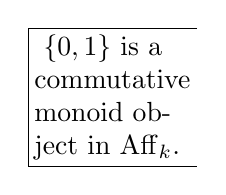
\begin{tikzpicture}[baseline=(note.base)]
\node[anchor=north west,align=left,text width=1.99cm,inner sep=2pt] (note) at (0,0)
{$\therefore\ \{0,1\}$ is a commutative monoid object in $\mathrm{Aff}_k$.};
\draw (note.north east)--(note.north west)--(note.south west)--(note.south east);
\end{tikzpicture}}

But $\{0,1\}(k)$ can't be a group object in sets.
\[
\begin{aligned}
&\text{\rq\rq}\\[-2pt]
&\{P_1,P_2\}.
\end{aligned}
\]

Moreover $A$ can't be given a co-inversion or antipodal map. One way of characterizing the inverse \inserted{$\sigma$} for commut gps is that $\exists\,\sigma:G\longrightarrow G$ \unsure{sud|such} that
\diagram{\begin{minipage}[t]{.47\linewidth}\vspace{0pt}\centering
\begin{tikzcd}[ampersand replacement=\&,row sep=large,column sep=small]
G\arrow[r,"{I_G\times\sigma}"] \&
G\times G\arrow[d,"\Pi","{\cdot}"{pos=.92,swap},"{\cdot}"{pos=.94}]\\
\& G
\end{tikzcd}
\end{minipage}\hfill
\begin{minipage}[t]{.48\linewidth}\vspace{0pt}
factors through the final then initial object :
\end{minipage}}
\diagram{\begin{tikzcd}[ampersand replacement=\&,row sep=2pt,column sep=3pt]
G\arrow[rr,"{I_G\times\sigma}"]\arrow[ddd] \& \& G\times G\arrow[ddd,"\Pi"] \& \&
 \text{i.e. that.}\arrow[dl,bend left=15]\\
\& {x\longmapsto(x,x^{-1})}\arrow[d,maps to] \& \& \vphantom{G} \&
 \begin{gathered}\text{commutes since}\\\text{the final }+\text{ initial}\\\text{objs coincide.}\end{gathered}\\
\& e.\& \& \&\\
e\arrow[rr,"{\cdot}"{pos=.94,below}] \& \& G \& \&
\end{tikzcd}}
% archive sheet number: 18
\clearpage

\scanpage{20}
\mspage{- 4 -}
\figure{
\begin{tikzpicture}[x=1mm,y=1mm]
\fill (0,0)--(1.1,.7)--(1.2,2.1)--(3.7,1.7)--(6.3,1.1)--(7.4,.2)--(7.5,-.4)--(3,.1)--cycle;
\fill (12.0,-1.1) circle[radius=.18];
\end{tikzpicture}}

On the coalgebra level $\exists\ A\xrightarrow{\unsure{\sigma_0|\sigma_o}} A$\quad s.t.
\diagram{\begin{minipage}[t]{.43\linewidth}\vspace{0pt}\centering
\begin{tikzcd}[ampersand replacement=\&,row sep=large,column sep=large]
 A \& A\otimes A\arrow[l,"{I_A\otimes\unsure{\sigma_0|\sigma_o}}"']\\
 k\arrow[u,"\text{structure}" description] \& A\arrow[l,"\text{counit}"]\arrow[u,"{\unsure{\Pi_0|\Pi_o}}"']
\end{tikzcd}
\end{minipage}\hfill
\begin{minipage}[t]{.54\linewidth}\vspace{0pt}\small
Suppose $\unsure{\sigma_0|\sigma_o}$ exists in this case :
\[
\unsure{\sigma_0|\sigma_o}(c,d)=(\sigma_{\unsure{0|o}1}(c,d),\sigma_{\unsure{0|o}2}(c,d)).
\]
Where.
\[
\sigma_{\unsure{0|o}i}=P_i\circ\unsure{\sigma_0|\sigma_o}.
\]
\end{minipage}}

\diagram{\begin{minipage}[t]{.55\linewidth}\vspace{0pt}
Now compute : the lower left route gives :
\end{minipage}\hfill
\begin{minipage}[t]{.42\linewidth}\vspace{0pt}\centering
\begin{tikzcd}[ampersand replacement=\&,column sep=small]
{(a,a)} \& \\
a\arrow[u,maps to,"{\text{structure.}}" description] \& {(a,b)}\arrow[l,maps to,"{P_1}"]
\end{tikzcd}
\end{minipage}}

\unsure{the|The} upper right route gives :
\diagram{\footnotesize\begin{tikzcd}[ampersand replacement=\&,column sep=small,row sep=small]
{(a,b)\cdot(\sigma_{\unsure{0|o}1}(1,0),\sigma_{\unsure{0|o}2}(1,0))} \& {(a,b)\otimes(1,0)+(1,1)\otimes(0,b)}\arrow[l,maps to]\\
{+} \&\\
{(1,1)\cdot(\sigma_{\unsure{0|o}1}(0,b),\sigma_{\unsure{0|o}2}(0,b)\unsure{{}^{\bullet}|{}^{\prime}}} \& {(a,b)}\arrow[uu,maps to]
\end{tikzcd}}
\[
\begin{aligned}
&\unsure{\text{\rq\rq}|\shortparallel}\\
&\bigl(a\sigma_{\unsure{0|o}1}(1,0)+\sigma_{\unsure{0|o}1}(0,b),\
 b\sigma_{\unsure{0|o}2}(1,0)+\sigma_{\unsure{0|o}2}(0,b).\bigr)
\end{aligned}
\]

This above is to be equal to $(a,a)$ for all $(a,b)$ ? Perhaps I am very confused! or perhaps $\mathrm{GL}(\unsure{n|u})_k$ \deleted{could}\inserted{should} be changed to $\mathcal E\mathit{nd}_k(M)$.

I'm enjoying the courses very much. Many thanks for letting me attend.\\
\hfill\unsure{F J|L J|E J} \unsure{Servedio|Servedis}\\
\hfill Dalhousie U., Halifax, N.S.\\
% archive sheet number: 19
\clearpage

\scanpage{21}
\figure{
\begin{tikzpicture}[x=1mm,y=1mm]
\fill[gray] (-20.2,1.65) circle (.1);
\fill (-4.3,-.55) circle (.18);
\draw[gray,very thin] (-4.1,-.48)--(-.7,-.08);
\fill (0,0)--(.4,.65)--(2.8,1.55)--(5.65,2)--(6.3,1)--(7.1,.35)--(6.3,.2)--(4.8,.5)--cycle;
\end{tikzpicture}}

\begin{center}Prof Grothendieck\hspace{1.6em}\unsure{.}\end{center}

\figure{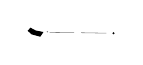
\begin{tikzpicture}[x=1mm,y=1mm]
\fill (0,.4)--(.35,.8)--(1,.45)--(2,.25)--(1.6,-.35)--(.5,-.05)--cycle;
\draw[gray,very thin] (2.8,.2)--(5.9,.16) (6.8,.16)--(10,.1);
\fill[gray] (2.5,.29) circle (.09);
\fill (10.9,.1) circle (.15);
\end{tikzpicture}}

\figure{\begin{tikzpicture}[x=1mm,y=1mm]
\draw[gray,very thin] (.2,.9) to[bend right=35] (.2,0);
\fill (10.9,.8)--(11.3,1.2)--(12,.9)--(11.85,.5)--(11,.55)--cycle;
\end{tikzpicture}}
% archive sheet number: 20.
\clearpage

\scanpage{22}
\uline{Rectification} \quad Si $G$ monoïde affine de t.f. sur corps $k$, on a une immersion fermée multiplicatif $G\mathbin{-}\mathbb M_{\unsure{n,k|n\,k}}$ (non $G\to\unsure{GL_{n,k}|Gl_{n,k}}$\unsure{)} car on peut montrer que si $G$ est un monoïde de pres. finie sur un anneau $k$, tel que les translations à g (disons sont des mono) - p.ex. s'il $\exists$ \unsure{mono|un} $G\longrightarrow G'$, $G'$ un \inserted{foncteur en} groupes - alors $\deleted{\unsure{G}}G$ est un objet gr-pe).

\figure{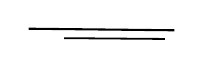
\begin{tikzpicture}[x=1cm,y=1cm]
\draw[line width=.75pt] (0,0) -- (1.85,-.02);
\draw[line width=.65pt] (.45,-.12) -- (1.73,-.13);
\end{tikzpicture}}

\deleted{$G$} $X$ schéma affine sur $k$, \deleted{\unsure{de|et}} de $k$-algèbre $\mathcal A$. On définit $\check{\mathcal A}=\mathrm{Dist}(X\deleted{)},k)$. On \unsure{a|.} le foncteur $\inserted{k'}\rightarrow\mathrm{Dist}(X,k')$, noté $\mathrm{Dis}(X)$, représentable par $\mathbb V(A)$. On a
% slanted
\reversemarginpar\margin{\tikz[baseline=-.3ex,x=1em,y=1em]{\draw[->] (.56,.85) to[out=-130,in=76] (0,-.55);} \uline{covariant}}\normalmarginpar
\[
\left\{\begin{aligned}
&\text{a)}\ \mathrm{Dist}(X)\ \text{fonctoriel en }X\quad
  (\text{comme Module sur }\unsure{\mathcal O|O|\mathbb O}_k)\\
&\text{b)}\ \mathrm{Dist}(X)\times\mathrm{Dist}Y)
  \xrightarrow[\unsure{\pi|\Pi}_{X,Y}]{\deleted{\unsure{\alpha|o}}}
  \mathrm{Dist}(X\times Y)\quad\text{bilinéaire}
\end{aligned}\right.
\]
[et universel pour les hom bilinéaires de $\mathrm{Dis}(X)\times\mathrm{Dis}(Y)$ dans un $\mathbb V(M)$] induisant en fait un isom
\[
\mathrm{Dist}(X)\boxtimes\mathrm{Dist}(Y)\simeq\mathrm{Dist}(X\times Y).
\]

c) On a une inclusion fonctorielle
\[
X\xrightarrow{\alpha_X}\mathrm{Dist}(X)
\]
[distribution ponctuelle, compatible avec passage au produit, i.e. on a comm. des
\diagram{\begin{tikzcd}[ampersand replacement=\&]
X\times Y \arrow[r,"\alpha_X\times\alpha_Y"] \arrow[dr,swap,"\unsure{\pi|\Pi}_{X\times Y}"] \& \unsure{\mathrm{Dist}}(X)\times\mathrm{Dist}(Y) \arrow[d,"\unsure{\pi|\Pi}_{X,Y}"]\\
\& \mathrm{Dist}(X\times Y)
\end{tikzcd}}

\deleted{Si $G$ est muni d'une loi de comp., $\mathrm{Dist}(G)$ aussi. \deleted{\unsure{Si}} Elle est unitaire sss celle de $\mathrm{Dist}(G)$ l'est} En fait on peut rêconstruire $X$ à partir de $\mathrm{Dist}(X)=\mathbb D$ et la structure supplémentaire
\[
D\overset{\Delta}{\unsure{\mathbin{-}|\longrightarrow}}D\boxtimes D
\]
\margin{$[\,V(A)\boxtimes V(B)\overset{\text{def}}{\simeq}V(A\otimes B)\,]$\newline
[NB $\boxtimes=\otimes$ si $A$ ou $B$ proj. de t.f.]}
% slanted
\reversemarginpar\margin{NB on rêconstitue $X$ à partir de $D$ muni \deleted{\unsure{la|du}}de l'application diagonale $D\to D\boxtimes D$ comm. ass. unitaire.}\normalmarginpar
doit être une ``application diagonale'' ass. comm. et counitaire [i.e. on a $D\xrightarrow{\varepsilon}\mathcal O$ \ldots.] comme formé des \deleted{\unsure{pts|gts}} $x\in\mathbb D(k')$ tels que
\[
\boxed{\Delta(x)=x\boxtimes x}
\]
% archive sheet number: 21

\cotefile{53}
\scanpage{23}
% loc 1–2, opening bracket
[\unsure{cet|cel} exprime que l'hom $A\mathrel{\tikz[baseline=-.3ex,x=1em,y=1em]{\draw[line width=.45pt] (0,0)--(1,0)--(1,.17);}}k'$ est un hom d'algèbres]

% loc 3–6, Si G
Si $G$ est muni d'une loi de comp. de $=$ $\mathrm{Dist}(D)$, celle-ci est ass. (comm) sss celle de $G$ l'est, et \deleted{unitaire} $G$ admet une unité bilatère ssi $\mathrm{Dist}(D)$ a une unité \deleted{\unsure{élément}} $e$ telle que $\delta(e)=e\boxtimes e$.

% loc 7–9, Dire que
Dire que $G$ opère sur un module $M$ \inserted{à g.)} signifie que $\mathrm{Dist}(G)$ y opère à gauche -- et cette opération étend celle de $G$.

% loc 10–14, NB
\uline{NB} Dans certains cas, $\mathrm{Dist}(X)$ se reconstitue à partir de $\mathrm{dist}(X,k)=\mathrm{Dst}(X)(k)$, p.ex. si $A$ est \deleted{\unsure{t.f.|de t.f.}} projectif de t.f. sur $k$, ou plus gén. si $A$ est somme de modules projectifs de t.f (p.ex. \deleted{\unsure{si}} $k$ un corps) -- mais alors il faut considérer $\mathrm{Dist}(x,k)$ comme module topologique.

% loc 15–20, Re NB
\uline{Re NB} Surtout intéressant pour monoïde. En plus \deleted{\unsure{de|du}} \inserted{du sous foncteur} $G$, $\mathrm{dist}(G)$ ' [resp $\mathrm{Dist}(G,k)$] contient toute l'information infinitésimale de $G$ : p.ex. l'\uline{algèbre de Lie} de $G$ est contenue dans $\mathrm{Dist}(G,k)$, -- \deleted{\unsure{et les op.}} sa loi de $[\,]$ est induite par le crochet de l'algèbre, et en car. pos sa puiss. pieme aussi -- de $=$ que l'hyperalgèbre.

\begin{center}\rule{1.6cm}{0.55pt}\end{center}
% loc 21, between the two rules
Cas des schémas constants : on retrouve l'\uline{algèbre} d'un groupe fini.

\begin{center}\rule{1.6cm}{0.55pt}\end{center}
% loc 22, second Cas
Cas du g.pe diagonalisable
% loc 23, A = k(M)
\[
 A=k(M)\quad\text{algèbre du groupe à coeff dans } k
\]
% loc 24–25, two paired rows
\diagram{\begin{tikzcd}[ampersand replacement=\&,column sep=small,row sep=large]
 A\otimes A \arrow[r,dash] \& A \& \text{provient de} \& M\times M \arrow[r] \& M \& \text{loi de groupe}\\
 A\otimes A \& \underset{\tikz[baseline,x=1em,y=1em]{\draw[gray,line width=.35pt] (.18,.12)--(.16,.02);\draw[gray,line width=.35pt] (.10,-.06) to[out=-90,in=0] (-.12,-.32);\draw[gray,line width=.35pt] (.16,-.22) to[out=-90,in=0] (-.15,-.49);}}{A} \arrow[l] \& \text{---} \& M\times M \& M \arrow[l,swap,"\substack{\text{application}\\\text{diagonale}}"] \&
\end{tikzcd}}
% loc 26–27, lowest two lines
\[
\begin{aligned}
 &\mathrm{Dist}(\mathbb D(M))(k)=\deleted{\unsure{*}}k^{M}\quad\text{avec la loi d'\uline{algèbre} \uline{produit}}\\
 &\qquad\text{[Combinaisons lin infinies de caractères]} \qquad
 \text{(\unsure{ne dépend pas de la str. additive de|ne dépend pas de la str. d'addition de} $M$)}
\end{aligned}
\]
% archive sheet number: 22

\scanpage{24}
% loc 1, heading
$A$ algèbre d'un $k$-\deleted{groupe}\inserted{monoïde} affine $G$

% loc 2
$M$ $k$ module

% loc 3–4, opération and brace
opération de $G$ on $M$ :
\[
 \text{i.e.}\quad G\longrightarrow
 \underline{\unsure{\mathrm{End}|\mathbb E\mathrm{nd}}}_{k}(M)
 =\underline{\mathbb E\mathrm{nd}}_{\unsure{\mathcal O|O|\mathbb O}}\overset{\deleted{\unsure{gxx|gx}}}{(W(M))}
 \quad
 \left\{\begin{aligned}1)&\ 1x=x\\2)&\ g(g'x)=gg'x\end{aligned}\right.
\]

% loc 5–8, Opération sans axiomes
``Opération sans axiomes'' correspond à
\[
\begin{aligned}
 &\deleted{\unsure{u:A\otimes M_{A}\to A\otimes_{k}M}}\quad
 u:M_A\mathrel{\mathop{\unsure{\text{---}|\to}}\limits_{\text{$A$ lin}}}M_A
 \qquad M_A\underset{\unsure{,|1}}{=}\tikz[baseline=(t.base)]{\node[inner sep=0pt](t){$A\otimes_k M$};\draw[thin](-.08,-.31) .. controls (.12,-.38) and (.05,.09) .. (.22,.21) .. controls (.38,.38) and (.58,.35) .. (.64,.30);}\\
 &\deleted{Ax} \\
 &\hspace{4em}\text{ou}\qquad u_0:M\longrightarrow
 \tikz[baseline=(t.base)]{\node[inner sep=0pt](t){$A\otimes_k M$};\draw[thin](-.12,-.30) .. controls (.10,-.39) and (.06,.06) .. (.25,.23) .. controls (.44,.35) and (.60,.31) .. (.64,.24);}
 \qquad\text{$k$-lin.}
\end{aligned}
\]

% loc 9, cancelled sentence
\deleted{L'axiome $1x=x$}

% loc 10–13, Si g
Si $g\in G(k')$ correspond à un hom de $k$-algèbres $A\overset{g}{\longrightarrow}k'$, alors $g_M$ sera l'endomorphisme \deleted{$\unsure{k'\otimes_A}$}\inserted{de} \tikz[baseline=(t.base)]{\node[inner sep=0pt](t){$(\deleted{g}k',\deleted{k}g)\otimes_A M$};\draw[thin](.18,-.29) .. controls (.35,-.33) and (.37,.08) .. (.50,.23) .. controls (.68,.43) and (.81,.36) .. (.81,.31);} \deleted{défini}\inserted{déduit} \deleted{\unsure{comme}}\inserted{de $u$} \deleted{$g\otimes_A i$} par changement de base, i.e. l'unique hom $M_{k'}\longrightarrow M_{k'}$ tel que le diagramme d'hom $A$-linéaires
% loc 14, bracketed fork and square
\diagram{\begin{tikzcd}[ampersand replacement=\&,column sep=2.9em,row sep=1.1em]
 \& M_A\arrow[rr,"u"]\arrow[dd,"{\tikz[baseline=(t.base)]{\node[inner sep=0pt](t){$\scriptstyle g\otimes\mathrm{id}_M$};\draw[thin](-.13,-.16) .. controls (-.06,-.19) and (-.09,.07) .. (.02,.16) .. controls (.13,.30) and (.22,.25) .. (.23,.22);}}"] \& \& M_A\arrow[dd,"{\tikz[baseline=(t.base)]{\node[inner sep=0pt](t){$\scriptstyle g\otimes\mathrm{id}_M$};\draw[thin](-.13,-.16) .. controls (-.06,-.19) and (-.09,.07) .. (.02,.16) .. controls (.13,.30) and (.22,.25) .. (.23,.22);}}"]\\
 \left[\vphantom{\dfrac{\dfrac{A}{A}}{\dfrac A A}}\right. M
 \arrow[ur]\arrow[dr] \&[-1.7em] \hspace{-2.2em}\left.\vphantom{\dfrac{\dfrac{A}{A}}{\dfrac A A}}\right] \& \& \\
 \& M_{k'}\arrow[rr,swap,"g_M"] \& \& M_{k'}
\end{tikzcd}}
% loc 15, after first diagram
est commutatif ; Mais cela signifie aussi que le diagramme
% loc 16, square
\diagram{\begin{tikzcd}[ampersand replacement=\&]
 M\arrow[r,"u_0"]\arrow[d,swap,"\mathrm{can}"] \& M\deleted{\unsure{{}_A}}\otimes A\arrow[d,"\mathrm{id}_M\otimes g"]\\
 M\deleted{\unsure{{}_k|{}_{k'}}}\otimes k'\arrow[r,swap,"g_M"] \& M\otimes k'
\end{tikzcd}}
% loc 17–19, est commutatif
est commutatif, ou encore, notant que la donnée de $g_M$ est équivalente à celle de $g_M^{\unsure{0|\circ}}=g_M\circ\mathrm{can}:M\mathrel{\tikz[baseline=-.3ex,x=1em,y=1em]{\draw[line width=.45pt] (0,0)--(1,0)--(1,.16);}}M\otimes k'$, à la \deleted{\unsure{fon.}} commutativité du
% loc 20, triangle
\diagram{\begin{tikzcd}[ampersand replacement=\&]
 M\arrow[r,"u_0"]\arrow[dr,swap,"g_M^{\unsure{0|\circ}}"] \& M\otimes A\arrow[d,"\unsure{\mathrm{id}|\mathrm{Id}}_M\otimes g"]\\
 \& M\otimes k'
\end{tikzcd}}

% loc 21–22, Pour traduire
Pour traduire l'axiome 1), on fait $k'=k$, $g=\deleted{\mathrm{id}_k}$ $(\varepsilon:A\longrightarrow k)$, et on trouve
% loc 23, circled 1 and triangle with equation
\diagram{\begin{tikzcd}[ampersand replacement=\&,column sep=2.8em,row sep=large]
 \tikz[baseline=(t.base)]{\node[draw,circle,inner sep=1.5pt](t){$1'$};} \& M\arrow[r,"u_0"]\arrow[dr,swap,near start,"\text{---}"{sloped}] \& M\otimes A\arrow[d,"\mathrm{id}_M\otimes\varepsilon"] \& \text{comm. i.e.}\\
 \& \& M \& (\mathrm{id}_M\otimes\varepsilon)u_0=\mathrm{id}_M
\end{tikzcd}}
% archive sheet number: 23

\scanpage{25}
% loc 1–2, Pour récrire
Pour récrire 2), on \deleted{écrit} prend $k'=A\otimes A$, et on choisit les deux hom
% loc 2, two parallel strokes
\diagram{\begin{tikzcd}[ampersand replacement=\&]
 \deleted{g} \& A^{\cdot}\arrow[r,dash,shift left=.55ex,"g"]\arrow[r,shift right=.55ex,swap,"g'"] \& A\otimes A \& \deleted{\unsure{g'}}\quad\text{donnés par}
\end{tikzcd}}
% loc 3, definitions
\[
 g(\lambda)=\lambda\otimes1,\quad g'(\lambda)=1\otimes\lambda
\]
% loc 4–7, et on écrit
et on écrit l'équation comme une égalité de deux endom. de $\deleted{M_{A\otimes A}}\ M_{k'}=M_{A\otimes A}$ qu'on va écrire -- puis on écrira l'égalité de leurs composés avec $M\overset{\mathrm{can}}{\longrightarrow}M_{A\otimes A}$ -- donc finalement il faudra définir deux $k$-hom $M\mathrel{\text{---}}M_{A\otimes A}$, savoir
% loc 8, two x maps
\[
 x\longmapsto gx'_{\deleted{\unsure{k'}}},\quad x\mathrel{\tikz[baseline=-.3ex,x=1em,y=1em]{\draw[line width=.45pt] (0,-.13)--(0,.13) (0,0)--(1,0)--(1,.14);}}g'x'_{\deleted{k}}
 \quad\text{(où }x'_k\text{ est l'image de }x\text{ dans }M_{k'}=M_{A\otimes A}\text{).}
\]

% loc 9–10, Or
Or
\[
 (gg')_M x'=(gg')_M^{\unsure{0|\circ}}x=(\mathrm{id}_M\otimes\unsure{gg|gg'})\circ u_0 \quad:
\]
% loc 10, upper box and element map
\diagram{\begin{tikzcd}[ampersand replacement=\&,column sep=large,execute at end picture={\draw ([xshift=-2pt,yshift=8pt]p.north west) -- ([xshift=7pt,yshift=8pt]q.north east) -- ([xshift=10pt,yshift=5pt]q.north east); \draw ([xshift=-5pt,yshift=2pt]p.north west) -- ([xshift=-5pt,yshift=-1pt]p.west|-r.south) -- ([xshift=-2pt,yshift=-4pt]p.west|-r.south); \draw ([xshift=8pt,yshift=1pt]q.east) -- ([xshift=8pt,yshift=-8pt]r.south east); \draw ([xshift=2pt,yshift=-6pt]p.west|-r.south) -- ([xshift=3pt,yshift=-6pt]r.south east); \draw[->] (s.north east) -- ([xshift=-1pt,yshift=-8pt]p.south west); \draw ([xshift=-3pt,yshift=-2pt]q.west) -- ([xshift=-3pt,yshift=2pt]q.west);}]
 \& |[alias=p]|M\arrow[r,dash,"u_0"] \& |[alias=q]|M\otimes A\arrow[d,swap,"\mathrm{id}_M\otimes\unsure{\pi|\Pi}"]\arrow[d,phantom,shift left=5ex,"\deleted{\unsure{(u_0\otimes\mathrm{id}_A)}}"] \& \deleted{\unsure{y\otimes\lambda}}\arrow[d,maps to]\\
 |[alias=s]|(gg')_M^0 \& \& |[alias=r]|M\otimes A\otimes A \& \deleted{\unsure{y\otimes\lambda\otimes1}}
\end{tikzcd}}
% loc 11, question
\[
 g_M(g'_Mx')=\,?
\]
% loc 12–13, Calculons and interline reading
Calculons $\underset{\substack{\unsure{\shortparallel|''}\\\unsure{(g'_M)^0x^{*}|(g'_M)^0x^{\varepsilon}}}}{g'_Mx'}\in M_{k'}$, c'est $(\mathrm{id}_M\otimes g')\deleted{(}(u_0(x))$ :
\diagram{\begin{tikzcd}[ampersand replacement=\&]
 M\arrow[r,"u_0"] \& M\otimes A\arrow[d] \& y\otimes\lambda\arrow[d]\arrow[d,phantom,swap,"\cdot"]\\
 \& M\otimes A\otimes A \& y\otimes1\otimes\lambda
\end{tikzcd}}
% loc 14–15, Donc and repeated par
Donc $g_M(g'_Mx')$ s'obtient en appliquant au résultat $g_M$, donné par par
% loc 16–17, g on two simple tensors
\[
\begin{aligned}
 &g_M(y\otimes\lambda\otimes\mu)=g_M^0(y)\,\lambda\otimes\mu
 =(\mathrm{id}_M\otimes g)(u_0(y))\,\lambda\otimes\mu\\
 &\text{\unsure{On.|en.} donc}\qquad g_M(y\otimes1\otimes\lambda)
 =\underset{\in M\otimes A\otimes1}{\underline{(\mathrm{id}_M\otimes g)u_0(y)}}\,1\otimes\lambda 
\end{aligned}
\]
% loc 18, lower box
donc
\diagram{\begin{tikzcd}[ampersand replacement=\&,column sep=large,execute at end picture={\draw ([xshift=-5pt,yshift=5pt]a.north west) -- ([xshift=15pt,yshift=5pt]a.north east) to[out=-85,in=180] ([xshift=26pt,yshift=-5pt]a.east) -- ([xshift=10pt,yshift=-5pt]c.east|-a.east); \draw ([xshift=-8pt,yshift=1pt]a.north west) -- ([xshift=-8pt,yshift=-5pt]b.south west); \draw ([xshift=8pt,yshift=1pt]c.east|-a.east) -- ([xshift=10pt,yshift=-5pt]c.south east); \draw ([xshift=-3pt,yshift=-11pt]b.south west) -- ([xshift=6pt,yshift=-11pt]c.south east);}]
 \& |[alias=a]|M\arrow[d,"u_0"] \& \\
 (g_Mg'_M)^0: \& |[alias=b]|M\otimes A\arrow[r,"u_0\otimes\mathrm{id}_A"] \& |[alias=c]|\underbrace{M\otimes A}\otimes A\\
 \& \deleted{\unsure{y\otimes\lambda}} \&
\end{tikzcd}}

% loc 19–20, Donc l'axiome
Donc l'axiome \deleted{de} 2 s'exprime comme
\diagram{\begin{tikzcd}[ampersand replacement=\&,column sep=large]
 \tikz[baseline=(t.base)]{\node[draw,circle,inner sep=1.6pt](t){$2'$};} \& M\arrow[r,"u_0"]\arrow[d,swap,"u_0"] \& M\otimes A\arrow[d,"\mathrm{id}_M\otimes\pi"] \& \text{\uline{commutatif}}\\
 \& M\otimes A\arrow[r,"u_0\otimes\mathrm{id}_A"] \& M\otimes A\otimes A \&
\end{tikzcd}}
% archive sheet number: 24

\scanpage{26}
% loc 1, struck NB and words above it
\deleted{\uline{NB} L'hom \inserted{de $k$-modules} $A\longrightarrow A\otimes A$ s'interprète comme un hom}

% loc 2–4, live NB and definition
\uline{NB} \unsure{Á|À} tout $k$-module $M$ associons le foncteur en $\unsure{\mathcal O|O|\mathbb O}$-modules
\[
 \unsure{V|\mathbb V|W}(M):\quad k'\longrightarrow\mathrm{Hom}_{k\text{-}\mathrm{Mod}}(M,k')
\]
qui dépend de façon \unsure{contravariante} de $M$. On trouve

% loc 5–7, a) and category map
a) $M\mathrel{\tikz[baseline=-.3ex,x=1em,y=1em]{\draw[line width=.45pt] (0,-.14)--(0,.14) (0,0)--(1,0) (1,-.09)--(1,.09);}}V(M)$ . est pl. fidèle \unsure{, i.e.,|, i.e.}
\[
 \mathrm{Mod}(k)^{\unsure{0|o|\circ}}\mathrel{\tikz[baseline=-.3ex,x=1em,y=1em]{\draw[line width=.45pt] (0,0)--(1,0) (1,-.12)--(1,.12);}}\mathrm{Mod}(\mathcal O)
\]
% loc 7–8, Hom and cancelled object below
\diagram{\begin{tikzcd}[ampersand replacement=\&,column sep=large]
 \deleted{b)}\quad\forall M,N \& \mathrm{Hom}_{K}(M,N)\arrow[r,"\substack{\alpha_{MN}\\[-2pt]\sim}"] \& \mathrm{Hom}_{\mathcal O}(W(N),W(M))\\
 \& \deleted{\unsure{W(M)(N\otimes{-})|W(M)(N{-})}}\arrow[u,Rightarrow] \&
\end{tikzcd}}
% loc 9, crossed prose before b)
\deleted{\unsure{Pour le voir définissons|Pour le voir définis un} hom \unsure{en sens inverse} $\unsure{f|\varphi}_{M,N}$ \unsure{.}}

% loc 10–11, b) and coupling
b) $\forall M,N$ \deleted{\unsure{$\xi$|:}} l'accouplement canonique
\[
 V(M)\otimes_{\mathcal O}V(N)\longrightarrow V(M\otimes_k N)\qquad,
\]
% loc 12–14, parenthesis and the smaller writing
\unsure{(|[}qui n'est pas un isom, car il n'est pas vrai que
\[
\begin{aligned}
 &\mathrm{Hom}_{k}(M',k')\otimes_{k'}\mathrm{Hom}_{k'}(N',k')
 \simeq\mathrm{Hom}_{k'}(M'\otimes_{k'}N',k')\quad ]\\
 &\qquad \overset{\unsure{\vee|\sim}}{M}'\otimes_{k'}\check N'\longrightarrow(M'\otimes_{k'}N')^{\vee}
\end{aligned}
\]
définit cependant, en prenant les $\mathrm{Hom}$ dans \deleted{\unsure{$P$}} un $V(P)$, un isom trifonctoriel
% loc 15–16, Hom diagram
\margin{\begin{tikzpicture}[x=1mm,y=1mm]\fill (0,0)--(.5,.2)--(1.2,.05)--(1.3,-.4)--(.7,-.8)--(.2,-.65)--(.15,-.25)--(0,-.2)--cycle;\end{tikzpicture}}
\diagram{\begin{tikzcd}[ampersand replacement=\&,column sep=large]
 \mathrm{Hom}_{\mathcal O}(V(M\otimes_k N),V(p))\arrow[r,"\sim"] \& \mathrm{Hom}(U(M)\otimes_{\mathcal O}V(N),V(p))\\
 \mathrm{Hom}_k(P,M\otimes N)\arrow[u,"\sim"'] \&
\end{tikzcd}}
% loc 17–19, On trouve
On trouve donc ainsi

\textbullet) Une loi de composition $\mathcal O$-linéaire sur un $V(A)$ ($A$ un $k$-module) est une comultiplication $A\overset{\unsure{\pi|\Pi}}{\longrightarrow}A\otimes A$.
% loc 20–22, unité and loi
Une unité \unsure{bilatère|bilatére} pour la loi de composition est une \tikz[baseline=(c.base)]{\node[inner sep=1pt](c){counité};\node[anchor=south,inner sep=1pt] at ([yshift=3pt]c.north){\inserted{augmentation}};\draw ([xshift=-2pt]c.south west) to[out=110,in=180] ([xshift=-2pt,yshift=2pt]c.north west) to[out=10,in=180] ([xshift=2pt,yshift=2pt]c.north east);} $A\overset{\varepsilon}{\longrightarrow}k$. \deleted{Une} La loi de composition est ass (comm) sss la loi d'algèbre est ass (comm).

% loc 23–25, Si M and its map
Si $M$ est un module, un accouplement $\mathcal O$-bilinéaire $V(A)\times W(M)\mathrel{\tikz[baseline=-.3ex,x=1em,y=1em]{\draw[line width=.45pt] (0,0)--(1,0)--(1,.15);}}V(M)$ est une application diagonale $M\longrightarrow A\otimes M$. \deleted{Si} $A$ muni d'une $\pi$ unitaire, alors
% loc 25–28, sloping margin note
% slanted
\margin{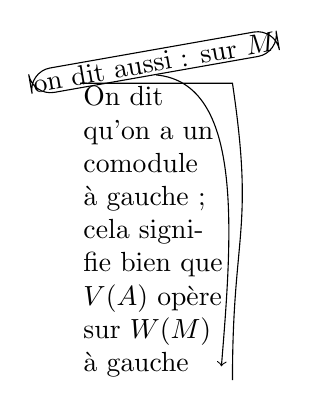
\begin{tikzpicture}[baseline=(m.base)]
 \node[align=left,text width=1.85cm,inner sep=1pt] (m) {On dit qu'on a un comodule à \uline{gauche} ; cela signifie \unsure{bien} que $V(A)$ opère sur $W(M)$ à gauche};
 \node[draw,rounded corners=8pt,align=center,inner sep=1pt,rotate=10,anchor=south] (g) at ([yshift=3pt]m.north) {\inserted{on dit aussi : sur $M$}};
 \draw[thin] (m.north west) .. controls ([xshift=5pt]m.north west) and (m.north) .. (m.north east) .. controls ([xshift=8pt]m.east) and (m.east) .. (m.south east);
 \draw[->,thin] (g.south) .. controls ([xshift=4pt]m.north east) and (m.east) .. ([xshift=-4pt,yshift=5pt]m.south east);
\end{tikzpicture}}
% loc 26–28, bottom lines
\deleted{loi de} l'accouplement est unitaire sss le diagramme \tikz[baseline=(t.base)]{\node[draw,circle,inner sep=1pt](t){$1'$};\fill ([xshift=3pt,yshift=-5pt]t.south east) circle (.7pt);} comm. ; \deleted{Si $A$ muni d'une} \inserted{Elle satisfait} $\mu(\lambda x)=(\lambda\mu)x$ (ass.) sss le diagramme $2'$ est commutatif.
% archive sheet number: 25

\scanpage{27}
% loc 1–4, Soit donc A
\deleted{\unsure{Soit|Si}}Soit donc $A$ une coalgèbre (ass, unit) et $M$ un comodule \tikz[baseline=(s.base)]{\node[inner sep=1pt](s){sur};\node[anchor=south east,inner sep=1pt] at ([xshift=4pt,yshift=6pt]s.north west){\inserted{à g.}};\draw ([xshift=-4pt,yshift=-2pt]s.south west) to[out=70,in=-110] ([xshift=6pt,yshift=17pt]s.north west);} la coalgèbre. $\check A=V(A)(k)$ opère à droite sur $\unsure{V|\mathbb V}(M)$, donc à gauche sur $W(M)$, ou ce qui revient au $=$, sur $M$, donc \deleted{$W($}$M$) devient une $\check A$-\deleted{alg}module. Si
% loc 5–7, xi and its action
\[
\begin{aligned}
 &\xi:A\mathrel{\tikz[baseline=-.3ex,x=1em,y=1em]{\draw[line width=.45pt] (0,0)--(1,0) (1,-.12)--(1,.12);}}k\qquad(k\text{-}\mathrm{lin})\qquad\in\check A,\ x\unsure{\vdash|\in}M\\
 &\text{on.}\qquad \xi\,.\,x=(\mathrm{id}_{\unsure{M|\mu}}\otimes\xi)(u_0(x))\\
 &\text{i.e.}\qquad \xi_M=(\mathrm{id}_M\otimes\xi)\circ u_0
\end{aligned}
\]
% loc 8–10, Notons and two Hom identifications
Notons que si $\deleted{\unsure{M}}A$ est \deleted{\illegible{1} , \unsure{sur tout|sur tous}}\inserted{projectif de t.f. sur $k$}, on a un isom
\[
\begin{aligned}
 &\deleted{M\otimes A\simeq\mathrm{Hom}\,\mathrm{cont}_k(}\\
 &M\otimes A\simeq\mathrm{Hom}_k(\check A,M)
\end{aligned}
\]
% loc 11–13, bracketed u0 and equivalence
donc la donnée de
\tikz[baseline=(h.base)]{\node[inner sep=2pt](h){$M\overset{u_0}{\longrightarrow}M\otimes_k A$};\draw (h.south west) .. controls +(-.3,0) and +(-.12,-.15) .. (h.north west) -- (h.north east) .. controls +(-.025,-.2) and +(-.1,-.35) .. (h.south east);}
[satisfaisant certaines conditions) \deleted{\unsure{revient}}\inserted{\uline{équivaut}} à la donnée de
\[
 \check A\longrightarrow\mathrm{Hom}_k(M,M)
\]
% loc 14–18, satisfying conditions, Le = argument
\margin{\begin{tikzpicture}[x=1mm,y=1mm]\fill (0,0)--(.9,.12)--(1.3,-.15)--(1.2,-.55)--(.4,-.8)--(.1,-.5)--cycle;\end{tikzpicture}}
satisfaisant aux conditions précédentes. On trouve alors que la donnée d'une structure de \inserted{$A$-}comodule \deleted{équivaut à} sur $M$. Le $=$ argument nous montre que sur le $k$-module $A$ projectif de t.f. $A$, la donnée d'une structure de coalgèbre (ass. \unsure{unit.|un?.}) équivaut à celle d'une str. d'algèbre (ass. unit.) sur $\check A$.

% loc 19–20, cancelled starts and interlinear replacements
\margin{\tikz[baseline=-.3ex]{\fill (0,0) circle (.65pt);}}
\deleted{Si $k$ est un corps}, On a un \unsure{rsult|résult|résultat} analogue \deleted{\unsure{sans supposer}}\inserted{si $A$ est libre}, \deleted{\unsure{$A$ de t.f., alors}} \inserted{p.ex. $k$ un corps} ; plus 
% loc 20–23, left margin and struck limit argument
% slanted
\margin{gén. si $A$ est somme directe de modules proj. de t.f.}
\deleted{$A$ de t.f. En effet, \unsure{on aura} $A=\underset{\mathrel{\tikz[baseline=-.3ex,x=1em,y=1em]{\draw[line width=.45pt] (0,0)--(1,0) (1,-.12)--(1,.12);}}}{\lim}_{\unsure{i|1}}\unsure{A_i|A'}$, \unsure{$A_i$|$A'$} les sous-modules de dim finie, donc $\check A=\underset{\longleftarrow}{\lim}\unsure{A_i|A_i'|A'}$ (lim. proj. de \unsure{limites|duals|duels|produits} de vectoriels de dim finie) de $\check A$}
% loc 23–26, convergence and Hom isomorphisms
Munissant $\check A$ de la topologie de la convergence simple, on aura
\[
 M\otimes_k A\simeq\mathrm{Hom}\,\mathrm{cont}_k(\check A,M)
\]
donc
\[
 \mathrm{Hom}(N,M\otimes_{\unsure{k|u}}A)
 \simeq\mathrm{Hom}\,\mathrm{cont}_{K}\bigl(\check A,\,
 \underbrace{\deleted{\unsure{H}}\mathrm{Hom}_k(N,M)}_{\substack{\text{muni de}\\\text{la top. de la}\\\text{conv. simple}}}\bigr)
\]
% loc 27–28, sentence continuing on scan 28
donc on trouve qu'une structure de comodule (ass. unit) sur $M$ revient à la donnée d'un
% archive sheet number: 26

\scanpage{28}
% loc 1–3, continuation at upper edge
structure de $\unsure{\widetilde A|\check A}$-module sur $M$ tel que pour tt $x\in M$, $\xi\mathrel{\tikz[baseline=-.3ex,x=1em,y=1em]{\draw[line width=.45pt] (0,-.13)--(0,.13) (0,0)--(1,0)--(1,.14);}}\xi x$ soit continue (i.e. s'annule sur un des $J_{\unsure{i|1|\prime}}\subset\check A\ \ldotp\ldotp\ldotp\ldotp\ \unsure{]|\exists}$. 
% loc 3–6, De =, on voit
De $=$, on voit que la donnée \deleted{\unsure{s}}d'une structure de coalgèbre \tikz[baseline=(s.base)]{\node[inner sep=1pt](s){sur le};\node[anchor=south,inner sep=1pt] at ([yshift=6pt]s.north){\inserted{(\unsure{ass. unit})}};\draw ([xshift=-4pt,yshift=-2pt]s.south west) to[out=75,in=180] ([yshift=5pt]s.north west) to[out=10,in=200] ([xshift=5pt,yshift=10pt]s.north east);} $k$-module libre $A$ revient à la donnée d'une \deleted{opération} structure de $k$-algèbre (ass. unitaire) sur $\check A$ qui soit \uline{continue}
% loc 7–8, car si; struck line and formula
[car si $\overset{\inserted{\unsure{k^{\Sigma}|k^{I}}}}{\overset{\tikz[baseline=-.4ex]{\node[rotate=90,inner sep=0pt]{\(\scriptscriptstyle\simeq\)};}}{P}},\overset{\inserted{k^{J}}}{\overset{\tikz[baseline=-.4ex]{\node[rotate=90,inner sep=0pt]{\(\scriptscriptstyle\simeq\)};}}{Q}},\overset{\inserted{k^{\Lambda}}}{\overset{\scriptscriptstyle\Vert}{R}}$ sont libres, \deleted{les \unsure{accouplements|applications} \tikz[baseline=(s.base)]{\node[inner sep=1pt](s){continus};\node[anchor=south west,inner sep=1pt] at ([xshift=-9pt,yshift=8pt]s.north west){\inserted{bil.}};\draw[->] ([xshift=-5pt,yshift=-2pt]s.south west) to[out=80,in=220] ([xshift=14pt,yshift=20pt]s.north west);} $\check P\times\check Q\unsure{\longrightarrow|-}\check R=\underset{\leftarrow}{\lim}_{\unsure{\alpha|\lambda}}\deleted{\unsure{R_{I}}}R_{\unsure{\Lambda_{\alpha}|\Lambda_2}}$.}
% loc 9–16, multiline Bil and Hom display
\[
\begin{aligned}
\unsure{\mathrm{bil}|\mathrm{Bil}}\,\tikz[baseline=(c.base)]{\node[inner sep=0pt](c){\(\mathrm{cont}_{k}\)};\fill ([xshift=1pt,yshift=1pt]c.south west) circle (.4pt);}\,\check P,\check Q;\check R)
 &\simeq \mathrm{Bil}\,\mathrm{cont}_{k}(\check P,\check Q;\underset{\leftarrow}{\lim}_{\gamma}(\check R_{\gamma}))\\
 &\simeq \underset{\leftarrow}{\lim}_{\gamma}\,[\mathrm{bil}\,\mathrm{cont}_{k}(\check P,\check Q;\check R_{\gamma})]\\
 &\simeq \underset{\leftarrow}{\lim}_{\gamma}\,\bigl[\underset{\mathrel{\tikz[baseline=-.3ex,x=1em,y=1em]{\draw[line width=.45pt] (0,0)--(1,0) (1,-.12)--(1,.12);}}}{\lim}_{\alpha,\beta}\,
 \mathrm{Bi}\underbrace{\mathrm{l}_{k}(\check P_{\alpha},\check Q_{\beta};\check R_{\gamma})}_{\mathrm{Hom}_{k}(\check P_{\alpha}\otimes\check Q_{\beta};\check R_{\gamma})\,]}\bigr]\\
 &\deleted{\simeq}\\
 &\simeq \underset{\leftarrow}{\lim}_{\gamma}\,\underset{\mathrel{\tikz[baseline=-.3ex,x=1em,y=1em]{\draw[line width=.45pt] (0,0)--(1,.05)--(1,-.10);}}}{\lim}_{\alpha,\beta}\,\mathrm{Hom}_{k}(R_{\gamma},P_{\alpha}\otimes Q_{\beta})\\
 &\simeq \underset{\leftarrow}{\lim}_{\gamma}\,\mathrm{Hom}_{k}(R_{\gamma},P\otimes Q)\\
 &\simeq \ldotp\,\mathrm{Hom}_{k}(R,P\otimes Q)\qquad !\quad ]
\end{aligned}
\]

% loc 17–21, On est dans
\margin{\begin{tikzpicture}[x=1mm,y=1mm]\fill (0,0)--(.8,.08)--(1,-.1)--(.95,-.4)--(.35,-.5)--(.05,-.7)--cycle;\end{tikzpicture}}
\deleted{On a également le même résultat} \inserted{On est dans le cas envisagé} si $A$ est limite \deleted{\unsure{projective}}inductive \uline{dénombrable} de sous-modules projectifs \tikz[baseline=(s.base)]{\node[inner sep=1pt](s){, à};\node[anchor=south west,inner sep=1pt] at ([xshift=-2pt,yshift=8pt]s.north west){\inserted{de t.f.}};\draw ([xshift=-3pt,yshift=-2pt]s.south west) to[out=85,in=175] ([xshift=1pt,yshift=7pt]s.north west) to[out=-5,in=200] ([xshift=14pt,yshift=14pt]s.north east);} morphismes de transition \deleted{ayant} des \deleted{suppléments} mon. univ. [i.e. ayant des inverses à g.] Mais dans le cas général, on ne peut oublier $V(A)$ \tikz[baseline=(s.base)]{\node[inner sep=1pt](s){au profit};\node[anchor=south west,inner sep=1pt] at ([xshift=-5pt,yshift=7pt]s.north west){\inserted{et ses opérations}};\draw ([xshift=-3pt,yshift=-2pt]s.south west) to[out=90,in=180] ([xshift=4pt,yshift=6pt]s.north west) to[out=5,in=220] ([xshift=14pt,yshift=15pt]s.north east);} de $\check A=V(A)(k)$ $\ldotp\ldotp\ldotp\ldotp$

% loc 22–27, Module quotient and quotient map
Module quotient et sous-module stable par une co-opération de la co-algèbre $A$ : Soit $M\overset{\unsure{g|f}}{\mathrel{\tikz[baseline=-.3ex,x=1em,y=1em]{\draw[line width=.45pt] (0,0)--(1,0) (1,-.12)--(1,.12);}}}N'$ un ép., alors $V(N)\subset V(M)$ mono, et il est clair ce que signifie que $V(N)$ est stable ; on dira alors que $N$ est stable par la coop. de $N$. Cel signifie aussi que $\exists$ un hom $N'\overset{\omega_{N'}}{\mathrel{\tikz[baseline=-.3ex,x=1em,y=1em]{\draw[line width=.45pt] (0,0)--(1,0) (1,-.12)--(1,.12);}}}N'\otimes A$ rendant comm.
% loc 27–28, commutative square
\diagram{\begin{tikzcd}[ampersand replacement=\&,column sep=large,execute at end picture={\draw ([xshift=-3pt,yshift=-2pt]nout.west)--([xshift=-3pt,yshift=2pt]nout.west);}]
M\arrow[r,"\omega_M"]\arrow[d] \& M\otimes A\arrow[d,"g\otimes\mathrm{id}_{A}"]\\
N'\arrow[r,dash,"\omega_{N'}"] \& |[alias=nout]| N'\otimes A
\end{tikzcd}}
% loc 29–30, last two lines
et cet $\omega_{N}$ est néc. unique et satisfait aux axiomes d'unité et associativité. Si $A$ est \unsure{un g.|un gp.|une alg.} affine
% archive sheet number: 27

\cotefile{53}
\scanpage{29}
% @ 1–4
d'un monoide affine $G$, cel signifie aussi qu'il existe une opération de $G$ sur $M'$ \deleted{qui} telle que $M\mathrel{\tikz[baseline=-.3ex,x=1em,y=1em]{\draw[line width=.45pt] (0,0)--(1,.05)--(1,-.10);}}M'$ soit comp. avec \unsure{son|ses} op., et il est clair \tikz[baseline=(s.base)]{\node[inner sep=1pt](s){(comme};\node[anchor=south east,inner sep=1pt] at ([xshift=-2pt,yshift=7pt]s.north west){\inserted{\unsure{directemt}}};\draw ([xshift=-10pt,yshift=-1pt]s.south west) to[out=70,in=190] ([xshift=-2pt,yshift=8pt]s.north west) to[out=10,in=250] ([xshift=13pt,yshift=15pt]s.north west);} $W(M)\mathrel{\tikz[baseline=-.3ex,x=1em,y=1em]{\draw[line width=.45pt] (0,0)--(1,.05)--(1,-.10);}}W(M')$ épi) que cette opération sera unique.

% @ 5–6
Si on a un. mono
\[
M''\overset{i}{\hookrightarrow}M
\]
% @ 7–9
alors il ne sera pas vrai en général que $V(M)\mathrel{\tikz[baseline=-.3ex,x=1em,y=1em]{\draw[line width=.45pt] (0,0)--(1,0) (1,-.12)--(1,.12);}}V(M'')$ soit surjectif, ni que $W(M'')\mathrel{\tikz[baseline=-.3ex,x=1em,y=1em]{\draw[line width=.45pt] (0,0)--(1,.05)--(1,-.10);}}W(M)$ soit injectif, donc \unsure{faute de|\deleted{faute de}} cette condition on a du mal à parler d'opération induite.
% @ 10–12
\deleted{\unsure{Crt il est|Cert il est}} On dira qu'il \uline{existe} une op. induite si on peut faire opérer $G$ sur $M''$ de telle façon que $M''\mathrel{\tikz[baseline=-.3ex,x=1em,y=1em]{\draw[line width=.45pt] (0,0)--(1,.05)--(1,-.10);}}M$ soit comp. aux opérations.
% @ 13–15
Mais il n'est plus clair que l'op ``induite'' soit unique ! En termes d'alg. comm., la question est de trouver un $\Delta_{M''}:M''\mathrel{\tikz[baseline=-.3ex,x=1em,y=1em]{\draw[line width=.45pt] (0,0)--(1,.05)--(1,-.10);}}M''\otimes A$ rendant commutatif
% @ 16–18 diagram
\margin{\begin{tikzpicture}[x=1mm,y=1mm]\fill (0,0) ellipse (.4mm and .2mm);\end{tikzpicture}}
\diagram{\begin{tikzcd}[ampersand replacement=\&,row sep=large,column sep=large]
 M'' \arrow[r,dash,"{u_{M''}\,?}",to path={.. controls +(right:4mm) and +(left:4mm) .. (\tikztotarget) \tikztonodes -- ++(-.3pt,-1.4pt)}] \& M''\otimes A \arrow[d,dash,"{i\otimes{\mathrm{id}}_A}",to path={-- (\tikztotarget) \tikztonodes -- ++(.7pt,-1.2pt)}] \\
 M \arrow[u,dash,"i"',to path={-- (\tikztotarget) \tikztonodes .. controls +(up:2pt) and +(up:1pt) .. ++(2.5pt,.2pt)}] \arrow[r,dash,"{u_M}",to path={-- (\tikztotarget) \tikztonodes -- ++(0pt,1.1pt)}] \& M\otimes A
\end{tikzcd}}

% @ 19–20
On peut dire que c'est uniquement déterminé pourvu que $i\otimes{\mathrm{id}}_A=i_A$ soit un mono,
% @ 20 interlinear
\figure{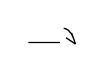
\begin{tikzpicture}[x=1mm,y=1mm]\draw[line width=.45pt] (0,0)--(4,0) (4.5,1.8) to[out=-10,in=110] (6,-.2) (6,-.2)--(5.5,1.2) (6,-.2)--(4.8,.6);\end{tikzpicture}}
\inserted{et si [$\unsure{i|j}\otimes{\mathrm{id}}_{A\otimes A}$ l'est aussi, alors la \unsure{condi.|condt.} \tikz[baseline=(s.base)]{\node[inner sep=1pt](s){\(u_M(M'')\subset\mathrm{Im}\,M''_{\otimes A}\)};\draw[->] ([xshift=-7pt,yshift=10pt]s.north west)--([xshift=-6pt,yshift=-3pt]s.north west)--([xshift=-2pt,yshift=9pt]s.north west);} est néc. et \uline{suffisante} pour la \deleted{\unsure{stabilité}} stabilité ; alors $M'$ est \unsure{stble|stbl} sss $M''$ l'est.}
% @ 21
\deleted{\unsure{batise|banise} \unsure{ces remarques}}. Les conditions envisagées sont ok dans les cas suivants :

% @ 22
a) $A$ est plat$/k$ (p.~ex. $k$ un corps)

% @ 22–24 right margin
\margin{\deleted{Alors les \unsure{c.s.} de \unsure{la} \unsure{q°} \unsure{s'appl.} \unsure{montrent} $u_M(M'')\subset\mathrm{Im}\,M''_{\otimes A}$.} 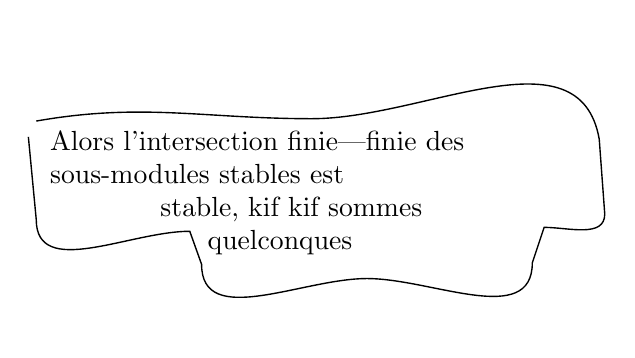
\begin{tikzpicture}[x=1cm,y=1cm]\node[anchor=north west,align=left,text width=7cm,inner sep=2pt](s) at (0,0){Alors l'intersection \unsure{\deleted{finie}|finie} des\\sous-modules stables est\\\hspace*{1.4cm}stable, kif kif sommes\\\hspace*{2cm}quelconques};\draw[line width=.5pt] (-.1,.05) to[out=10,in=180] (3.4,.08) to[out=0,in=100] (7.05,-.18)--(7.12,-1.13) to[out=-90,in=0] (6.35,-1.3)--(6.2,-1.75) to[out=-90,in=0] (4.1,-1.95) to[out=180,in=-90] (2,-1.77)--(1.85,-1.35) to[out=180,in=-90] (-.1,-1.2)--(-.2,-.15);\end{tikzpicture}}
% @ 23
b) $M/M''$ est \inserted{$\unsure{A|\wedge}$} plat

% @ 24
c) $M''$ facteur direct dans $M$.

% @ 24 left margin
% slanted
\margin{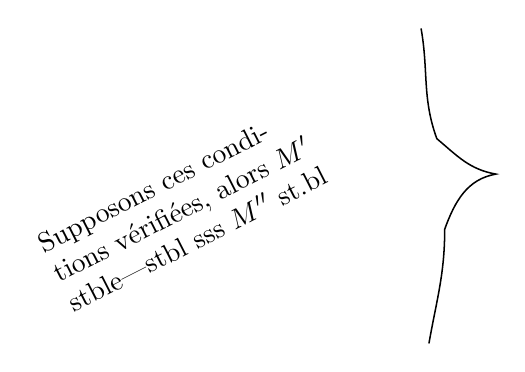
\begin{tikzpicture}[x=1cm,y=1cm]\node[rotate=27,align=left,text width=4.5cm,inner sep=2pt](s) at (0,0){\deleted{Supposons ces conditions vérifiées, alors $M'$ \unsure{stble|stbl} sss $M''$ st.bl}};\draw[line width=.55pt] (2.65,2.1) to[out=-80,in=110] (2.85,.7) to[out=-40,in=170] (3.6,.25) to[out=190,in=70] (2.95,-.45) to[out=-90,in=80] (2.75,-1.9);\end{tikzpicture}}
% @ 25
\deleted{ou $A$ \unsure{libre bien}.}

% @ 26–29
Dans le cas $A$ libre [plus gén. somme de modules proj. de t. f.] on voit que $M'$ est \unsure{st.bl|st.ble} sss $M'$ est \deleted{stable sous l'action de $\check{A}$.} un sous-$\check{A}$-module. On trouve donc

% @ 30–32
\uline{Proposition} Si $A$ est somme de modules proj. de t. f., alors un sous-$k$-module \deleted{de} $A$-comodule est st.bl sss il est \deleted{stable sous l'op.} \unsure{un|est} sous $\unsure{\check{A}|\tilde{A}}$-module.
% archive sheet number: 28

\scanpage{30}
% @ 1–4
\uline{Corollaire} 1 \unsure{Tout|Pour} \deleted{\unsure{tout}} sous-module $M'$ de $M$, il y a un plus petit sous-module \tikz[baseline=(s.base)]{\node[inner sep=1pt](s){\unsure{stble|stbl}};\node[anchor=south east,inner sep=1pt] at ([xshift=4pt,yshift=6pt]s.north west){\inserted{$M'^{\unsure{\vcenter{\hbox{\tikz[x=1ex,y=1ex]{\draw[line width=.11ex,line cap=round,line join=round] (.57,.90) .. controls (.45,.76) and (.24,.53) .. (.15,.35) .. controls (.35,.35) and (.56,.45) .. (.73,.41) .. controls (.64,.2) and (.45,.03) .. (.32,-.14);}}}|\natural|\sharp|\mathrm{s}}}$}};\draw ([xshift=-8pt,yshift=-2pt]s.south west) to[out=80,in=200] ([xshift=1pt,yshift=7pt]s.north west) to[out=20,in=250] ([xshift=8pt,yshift=13pt]s.north west);} de $M$ qui contienne $M'$, et c'est aussi la sous $\check A$-algèbre engendrée. Si $M'$ est de t.f. \deleted{sur} $k$, $M'^{\vcenter{\hbox{\tikz[x=1ex,y=1ex]{\draw[line width=.11ex,line cap=round,line join=round] (.57,.90) .. controls (.45,.76) and (.24,.53) .. (.15,.35) .. controls (.35,.35) and (.56,.45) .. (.73,.41) .. controls (.64,.2) and (.45,.03) .. (.32,-.14);}}}}$ aussi, \deleted{donc} \deleted{\unsure{M}}% end of the crossed group

% @ 5–6
\uline{Corollaire 2} $M$ est limite inductive filtr.\deleted{\unsure{$\to$|t}} de ses sous-modules de t. f. \uline{stbles}, \deleted{\unsure{par}}

% @ 7–8
\deleted{\uline{Corollaire 3}} \deleted{\unsure{M}} \deleted{Appliquons} Considérons $A$ comme bicomodule sur lui-même à g. et à droite, \deleted{plus} donc comme bi-module sur $\check A$,
% @ 9–12
\deleted{Alors pour \unsure{H|tt} $x$, les \unsure{s.}} considérons les sous-bi-modules $B\subset A$. \deleted{On voit que pour} Appliquant Cor 1 et 2 \deleted{les sous-\unsure{bi-mod.}} \deleted{\unsure{$A$|à} $A$ considéré comme $A$} à \tikz[baseline=(s.base)]{\node[inner sep=1pt](s){\(A\otimes A^{\mathrm{o}}\)};\node[anchor=south west,inner sep=1pt](a) at ([xshift=-5pt,yshift=8pt]s.north west){\inserted{la coalgèbre produit ; ($A^{\mathrm{o}}$ l'opposée de $A$)}};\draw ([xshift=-13pt,yshift=-3pt]s.south west) to[out=75,in=190] (a.south west) to[out=5,in=180] ([xshift=3pt,yshift=-2pt]a.south east) to[out=0,in=-90] ([xshift=4pt,yshift=3pt]a.south east);} et au module $A$ pour celle-ci, ou raisonnant directement, on trouve

% @ 13–16
\uline{Cor 3} \deleted{\unsure{Tout} \unsure{bi} \unsure{linéi}} Tout sous-bi-module $B$ de $A$ est contenu dans un plus-petit sous-bi-module $B^{\vcenter{\hbox{\tikz[x=1ex,y=1ex]{\draw[line width=.11ex,line cap=round,line join=round] (.57,.90) .. controls (.45,.76) and (.24,.53) .. (.15,.35) .. controls (.35,.35) and (.56,.45) .. (.73,.41) .. controls (.64,.2) and (.45,.03) .. (.32,-.14);}}}}$ \deleted{\unsure{stable|stble} par} \deleted{\inserted{\unsure{qui est}}} st.bl à g. et à droite (savoir le sous-$\check A$-bi-module engendré), et si $B$ est de t. f. sur $k$, $B^{\vcenter{\hbox{\tikz[x=1ex,y=1ex]{\draw[line width=.11ex,line cap=round,line join=round] (.57,.90) .. controls (.45,.76) and (.24,.53) .. (.15,.35) .. controls (.35,.35) and (.56,.45) .. (.73,.41) .. controls (.64,.2) and (.45,.03) .. (.32,-.14);}}}}$ aussi.
% @ 17–18
Donc $A=\underset{\mathrel{\tikz[baseline=-.3ex,x=1em,y=1em]{\draw[line width=.45pt] (0,0)--(1,.05)--(1,-.10);}}}{\mathrm{lim}}\,A_i$, les $A_i$ étant st.bles à g. et à droite.

% @ 19–23
Or cette st.bilité \tikz[baseline=(s.base)]{\node[inner sep=1pt](s){signifie};\node[anchor=south east,inner sep=1pt](a) at ([xshift=3pt,yshift=6pt]s.north west){\inserted{pour un $B$ donné}};\draw ([xshift=-2pt,yshift=-1pt]s.south west) to[out=90,in=180] ([xshift=2pt,yshift=-2pt]a.south west)--([xshift=-1pt,yshift=-2pt]a.south east) to[out=0,in=-90] ([xshift=2pt,yshift=1pt]a.south east);} que $\unsure{\Pi|\pi}:A\mathrel{\tikz[baseline=-.3ex,x=1em,y=1em]{\draw[line width=.45pt] (0,0)--(1,.05)--(1,-.10);}}A\otimes A$ envoie $B$ dans $(B\otimes A)\unsure{.|,}\cap(A\otimes B)$. Si \deleted{$B$ \unsure{est}} $A/B$ est plat sur $k$ (p ex $k$ un corps) cel signifie aussi que $\Pi$ envoie $B$ dans $B\otimes B$, ou encore qu'il y a une structure de co-algèbre induite. On trouve donc

% @ 24–26
\uline{Cor. 4} Toute coalgèbre \tikz[baseline=(s.base)]{\node[inner sep=1pt](s){sur};\node[anchor=south east,inner sep=1pt] at ([xshift=2pt,yshift=7pt]s.north west){\inserted{$\unsure{A|\wedge}$}};\draw ([xshift=-8pt,yshift=-5pt]s.south west) to[out=90,in=200] ([xshift=-2pt,yshift=5pt]s.north west) to[out=20,in=270] ([xshift=6pt,yshift=11pt]s.north west);} un corps est \tikz[baseline=(s.base)]{\node[inner sep=1pt](s){\(\underset{\mathrel{\tikz[baseline=-.3ex,x=1em,y=1em]{\draw[line width=.45pt] (0,0)--(1,.05)--(1,-.10);}}}{\mathrm{lim}}\)};\node[anchor=south west,inner sep=1pt] at ([xshift=3pt,yshift=6pt]s.north east){\inserted{fil.}};\draw ([xshift=5pt,yshift=-2pt]s.south east) to[out=65,in=225] ([xshift=19pt,yshift=17pt]s.north east);} de coalgèbres de t. f., donc $\check A$ est \tikz[baseline=(s.base)]{\node[inner sep=1pt](s){\(\underset{\leftarrow}{\mathrm{lim}}\)};\node[anchor=south west,inner sep=1pt](a) at ([xshift=-1pt,yshift=7pt]s.north west){\inserted{fil. stricte}};\draw ([xshift=4pt,yshift=-3pt]s.south east) to[out=90,in=190] ([xshift=4pt,yshift=-1pt]a.south east) to[out=10,in=-90] ([xshift=9pt,yshift=6pt]a.south east);} d'algèbres finies sur $k$.
% archive sheet number: 29

\scanpage{31}
% @ 1
\uline{Prop.} $G$ \deleted{\unsure{groupe alg.}} \tikz[baseline=(s.base)]{\node[inner sep=1pt](s){affine};\node[anchor=south east,inner sep=1pt](a) at ([xshift=2pt,yshift=7pt]s.north west){\inserted{groupe \inserted{(monoïde)}}};\draw ([xshift=-8pt,yshift=-4pt]s.south west) to[out=90,in=190] ([xshift=1pt,yshift=-2pt]a.south west)--([xshift=1pt,yshift=-2pt]a.south east) to[out=0,in=-90] ([xshift=3pt,yshift=3pt]a.south east);} sur le corps $k$. Alors

% @ 2–3
a) $G$ \deleted{\unsure{G}} est limite projective \tikz[baseline=(s.base)]{\node[inner sep=1pt](s){de};\node[anchor=south east,inner sep=1pt](a) at ([xshift=2pt,yshift=7pt]s.north west){\inserted{\unsure{filtr. str|filtr. de|filtrante}}};\draw ([xshift=-8pt,yshift=-4pt]s.south west) to[out=90,in=190] ([xshift=1pt,yshift=-2pt]a.south west)--([xshift=1pt,yshift=-2pt]a.south east) to[out=0,in=-90] ([xshift=3pt,yshift=3pt]a.south east);} \tikz[baseline=(s.base)]{\node[inner sep=1pt](s){(monoïdes)};\node[anchor=south east,inner sep=1pt](a) at ([xshift=2pt,yshift=7pt]s.north west){\inserted{groupes}};\draw ([xshift=-8pt,yshift=-4pt]s.south west) to[out=90,in=190] ([xshift=1pt,yshift=-2pt]a.south west)--([xshift=1pt,yshift=-2pt]a.south east) to[out=0,in=-90] ([xshift=3pt,yshift=3pt]a.south east);} affines de t.f. sur $k$, \deleted{\unsure{et}} \deleted{\unsure{b} avec des morphismes}

% @ 4–5
b) Si $G$ est un monoïde \tikz[baseline=(s.base)]{\node[inner sep=1pt](s){affine};\node[anchor=south east,inner sep=1pt](a) at ([xshift=2pt,yshift=7pt]s.north west){\inserted{(\unsure{grpe|groupe})}};\draw ([xshift=-8pt,yshift=-4pt]s.south west) to[out=90,in=190] ([xshift=1pt,yshift=-2pt]a.south west)--([xshift=1pt,yshift=-2pt]a.south east) to[out=0,in=-90] ([xshift=3pt,yshift=3pt]a.south east);} de t.f. sur $k$, on peut trouver un \deleted{\unsure{i|imm.}} entier $n$ et une immersion fermée
% @ 6
\[
 G\mathrel{\tikz[baseline=-.3ex,x=1em,y=1em]{\draw[line width=.45pt] (0,0)--(1,0) (1,-.12)--(1,.12);}}\tikz[baseline=(s.base)]{\node[inner sep=1pt](s){\(\deleted{\unsure{\mathrm{GL}}}M(n)_{k}^{\unsure{\times|x}}\)};\node[anchor=north,inner sep=1pt](a) at ([xshift=12pt,yshift=-15pt]s.south){\inserted{schéma de matrices $n\times n$}};\draw[->] ([xshift=3pt,yshift=-1pt]s.south) to[out=-100,in=170] ([xshift=-12pt,yshift=2pt]a.north);}.\quad
 (\text{resp. }G\to\mathrm{GL}(n))
\]

% @ 7–9
\uline{Dém} $G\longleftrightarrow A$, \deleted{\unsure{et}} et $A=\underset{i}{\underset{\mathrel{\tikz[baseline=-.3ex,x=1em,y=1em]{\draw[line width=.45pt] (0,0)--(1,0) (1,-.12)--(1,.12);}}}{\mathrm{lim}}}\,A_i$, $A_i$ les sous-algèbres de t. f. de $A$. On s'intéresse aux sous-algèbres $B$ qui sont ``st.bles'' par $\unsure{\Pi|\pi}:A\otimes A$, or il est clair que si
% @ 10–12
$M\subset A$ est st.bl sous $\Pi$, alors aussi la sous-algèbre \tikz[baseline=(s.base)]{\node[inner sep=1pt](s){qu'elle};\node[anchor=south east,inner sep=1pt](a) at ([xshift=2pt,yshift=7pt]s.north west){\inserted{$B$}};\draw ([xshift=-8pt,yshift=-4pt]s.south west) to[out=90,in=190] ([xshift=1pt,yshift=-2pt]a.south west)--([xshift=1pt,yshift=-2pt]a.south east) to[out=0,in=-90] ([xshift=3pt,yshift=3pt]a.south east);} engendre. Donc le corollaire 2 nous est que l'on peut supposer les $A_i$ stbles par $\Pi$. Si $G$ un groupe, d'où un antipodisme
% @ 13–17
$\sigma$ de $A$, alors si $M$ st.bl sous $\sigma$, alors l'algèbre $B$ aussi. Or si $M$ stable par $\Pi$, $\sigma M$ aussi [$M$ sous-module à g. \tikz[baseline=(s.base)]{\node[inner sep=1pt](s){sur};\node[anchor=south east,inner sep=1pt](a) at ([xshift=2pt,yshift=7pt]s.north west){\inserted{(à dr)}};\draw ([xshift=-8pt,yshift=-4pt]s.south west) to[out=90,in=190] ([xshift=1pt,yshift=-2pt]a.south west)--([xshift=1pt,yshift=-2pt]a.south east) to[out=0,in=-90] ([xshift=3pt,yshift=3pt]a.south east);} $\check A$ $\Longleftrightarrow$ $\sigma M$ sous-module à dr (g) sur $\check A$] donc $M+\sigma M$ aussi, donc on peut supposer les $A_i$ de plus st.ble par $\sigma$, donc les $G_i$ sont des groupes.

% @ 18–21
Supposons \unsure{maintnt|maintenant} $A$ de t-f., donc on a un sous $k$-module \tikz[baseline=(s.base)]{\node[inner sep=1pt](s){$M$};\node[anchor=south east,inner sep=1pt](a) at ([xshift=2pt,yshift=7pt]s.north west){\inserted{de tf.}};\draw ([xshift=-8pt,yshift=-4pt]s.south west) to[out=90,in=190] ([xshift=1pt,yshift=-2pt]a.south west)--([xshift=1pt,yshift=-2pt]a.south east) to[out=0,in=-90] ([xshift=3pt,yshift=3pt]a.south east);} de $A$ qui engendre $A$ comme algèbre. \deleted{Considérons} On peut supposer $M$ \unsure{st.bl|stbl} par $\check A$ à \tikz[baseline=(s.base)]{\node[inner sep=1pt](s){\deleted{\unsure{droite}}};\node[anchor=south,inner sep=1pt] at ([yshift=3pt]s.north){\deleted{\unsure{gauche|g.}}};\node[anchor=north,inner sep=1pt] at ([yshift=-3pt]s.south){\inserted{droite}};} donc que $G$ y opère à \deleted{\unsure{gauche}} \inserted{droite}. Donc
% @ 22
\[
 G\longrightarrow\deleted{\unsure{\mathrm{GL}|{\mathrm{End}}}}\,\underline{\mathrm{Aut}}_{k}(M)\quad(\simeq\mathrm{GL}(n)_{k})
\]
% @ 23–24
Av $n=\dim M$. Prouvons que c'est un mono. \deleted{\unsure{On a}} Soit \deleted{$\unsure{g}\ \varepsilon(f)\ \unsure{=0}$} Considérons \tikz[baseline=(s.base)]{\node[inner sep=1pt](s){la};\node[anchor=south east,inner sep=1pt](a) at ([xshift=2pt,yshift=7pt]s.north west){\inserted{pour \unsure{tt|$\forall$} $\varphi\in M$}};\draw ([xshift=-8pt,yshift=-4pt]s.south west) to[out=90,in=190] ([xshift=1pt,yshift=-2pt]a.south west)--([xshift=1pt,yshift=-2pt]a.south east) to[out=0,in=-90] ([xshift=3pt,yshift=3pt]a.south east);} fonction sur $G$
% @ 25
\[
 G\longrightarrow\mathbb E\qquad \deleted{\unsure{g}}\quad
 g\longmapsto\varepsilon(g.\varphi)=(g\varphi)(1)=\varphi(g)
\]
% @ 26–28
\deleted{\unsure{donc} $\unsure{E|k}'$} Donc \deleted{\unsure{g}} $M\unsure{\subset|\in}\mathrm{Im}\,[\text{anneau }\tikz[baseline=(s.base)]{\node[inner sep=1pt](s){de};\node[anchor=south east,inner sep=1pt](a) at ([xshift=-2pt,yshift=7pt]s.north west){\inserted{affine}};\draw ([xshift=-12pt,yshift=-2pt]s.north west) to[out=100,in=0] ([xshift=-10pt,yshift=-2pt]a.south east);\draw ([xshift=-12pt,yshift=-2pt]s.north west)--([xshift=-2pt,yshift=10pt]s.north west);}\,\underline{\mathrm{End}}_k(M)\mathrel{\tikz[baseline=-.3ex,x=1em,y=1em]{\draw[line width=.45pt] (0,0)--(1,0) (1,-.12)--(1,.12);}}A]$ \deleted{\unsure{donc}} \unsure{L'anneau|l'anneau} affine de $\underline{\tikz[baseline=(e.base)]{\node[inner sep=0pt](e){\(\mathrm E\)};\draw ([xshift=1pt,yshift=2pt]e.north west) to[out=20,in=140] ([xshift=2pt,yshift=0pt]e.north east);}\mathrm{nd}}_k(M)$ et a fortiori celui de $\mathrm{GL}(n)$ s'en va \uline{sur} $A$, OK.
% archive sheet number: 30

\scanpage{32}
% @ 1–3
Si $A$ est l'algèbre \tikz[baseline=(s.base)]{\node[inner sep=1pt](s){d'un};\node[anchor=south east,inner sep=1pt](a) at ([xshift=2pt,yshift=7pt]s.north west){\inserted{affine}};\draw ([xshift=-8pt,yshift=-4pt]s.south west) to[out=90,in=190] ([xshift=1pt,yshift=-2pt]a.south west)--([xshift=1pt,yshift=-2pt]a.south east) to[out=0,in=-90] ([xshift=3pt,yshift=3pt]a.south east);} \unsure{monoide|monoïde} \tikz[baseline=(s.base)]{\node[inner sep=1pt](s){sur};\node[anchor=south east,inner sep=1pt](a) at ([xshift=2pt,yshift=7pt]s.north west){\inserted{affine $G$}};\draw ([xshift=-8pt,yshift=-4pt]s.south west) to[out=90,in=190] ([xshift=1pt,yshift=-2pt]a.south west)--([xshift=1pt,yshift=-2pt]a.south east) to[out=0,in=-90] ([xshift=3pt,yshift=3pt]a.south east);} $k$, [i.e. $A$ est muni, en plus de la comultiplication $\unsure{\Pi|\pi}$ \tikz[baseline=(s.base)]{\node[inner sep=1pt](s){d'une};\node[anchor=south east,inner sep=1pt](a) at ([xshift=2pt,yshift=7pt]s.north west){\inserted{assoc. et unitaire}};\draw ([xshift=-8pt,yshift=-4pt]s.south west) to[out=90,in=190] ([xshift=1pt,yshift=-2pt]a.south west)--([xshift=1pt,yshift=-2pt]a.south east) to[out=0,in=-90] ([xshift=3pt,yshift=3pt]a.south east);} multiplication bilinéaire \inserted{ass. unitaire} \deleted{\unsure{qui en fait un|qui en fait une}} qui est de plus \uline{commutative}, et $\Pi$ est un
% @ 4–8
hom d'algèbre] alors $\forall\,k'$, les \unsure{élmts|éléments} de \tikz[baseline=(s.base)]{\node[inner sep=1pt](s){$\mathrm{Hom}_{k\text{-mod.}}(A,k')$};\node[anchor=south east,inner sep=1pt](a) at ([xshift=2pt,yshift=7pt]s.north west){\inserted{$V(A)(k')=$}};\draw ([xshift=-8pt,yshift=-4pt]s.south west) to[out=90,in=190] ([xshift=1pt,yshift=-2pt]a.south west)--([xshift=1pt,yshift=-2pt]a.south east) to[out=0,in=-90] ([xshift=3pt,yshift=3pt]a.south east);} \tikz[baseline=(s.base)]{\node[inner sep=1pt](s){sont};\node[anchor=south east,inner sep=1pt](a) at ([xshift=2pt,yshift=7pt]s.north west){\inserted{i.e. les hom $k$-lin $A\to k'$}};\draw ([xshift=-8pt,yshift=-4pt]s.south west) to[out=90,in=190] ([xshift=1pt,yshift=-2pt]a.south west)--([xshift=1pt,yshift=-2pt]a.south east) to[out=0,in=-90] ([xshift=3pt,yshift=3pt]a.south east);} \unsure{appelés|appelées} les ``\uline{distributions} de $G$ à \deleted{\unsure{valeurs}} coeff dans $k'$'', notés $\mathrm{Dist}(G)(k')$\tikz[baseline=(s.base)]{\node[inner sep=1pt](s){.};\node[anchor=south east,inner sep=1pt](a) at ([xshift=2pt,yshift=7pt]s.north west){\inserted{[algèbre des distributions]}};\draw ([xshift=-8pt,yshift=-4pt]s.south west) to[out=90,in=190] ([xshift=1pt,yshift=-2pt]a.south west)--([xshift=1pt,yshift=-2pt]a.south east) to[out=0,in=-90] ([xshift=3pt,yshift=3pt]a.south east);} Donc \deleted{\unsure{on a}} elles forment une $k'$-algèbre [``l'algèbre du \deleted{groupe} \inserted{monoïde} \deleted{\unsure{G}} $G$ à coeff dans $k'$''] et on aura une \unsure{inclusion|l'inclusion} de monoïdes
% @ 9
\[
 G\deleted{(k')}\hookrightarrow\mathrm{Dist}(G)(k')^{\unsure{\times|x}}
\]
% @ 10–11
et si $G$ est un groupe
\[
 G(k')\hookrightarrow\mathrm{Dist}(G)(k')^{*}
\]
\margin{\tikz[baseline=-.2ex,x=1em,y=1em]{\draw (.36,.77)--(.12,.77)--(.12,-.08)--(.34,-.08); \draw (.12,.68) to[out=-125,in=180] (.09,-.01) to[out=-10,in=0] (.30,-.11);}\unsure{pratiquement|pratiquemt} jamais un isom]}

% @ 11 left margin
% margin note written sideways
\margin{\diagram{\rotatebox{90}{\begin{tikzcd}[ampersand replacement=\&,column sep=small,row sep=small,font=\scriptsize]
 \mathrm{Dist}(X) \arrow[r,"{\Pi}"] \& \mathrm{Dist}(X)\times\mathrm{Dist}(X) \& \Pi(x)={} \\
 \deleted{e} \arrow[r,phantom,"{\deleted{\to}}"] \& \deleted{\mathrm{Dist}(X)} \& \\
 e \arrow[uu] \& \&
\end{tikzcd}}}}

% @ 12–13
\figure{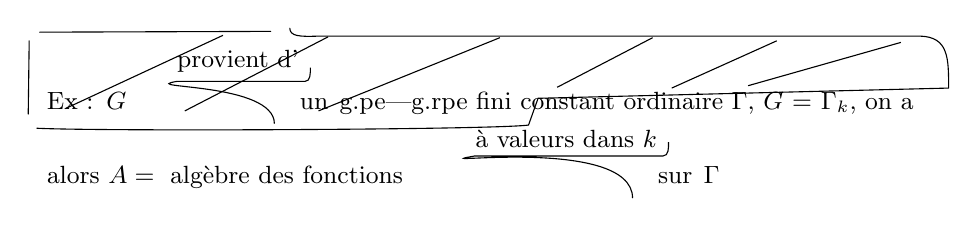
\begin{tikzpicture}[x=\linewidth,y=1cm]
\node[anchor=north west,inner sep=0pt,text width=.92\linewidth,font=\small] at (.025,.02)
 {\deleted{Ex : $G$ \tikz[baseline=(s.base)]{\node[inner sep=1pt](s){un};\node[anchor=south east,inner sep=1pt](a) at ([xshift=2pt,yshift=7pt]s.north west){\inserted{provient d'}};\draw ([xshift=-8pt,yshift=-4pt]s.south west) to[out=90,in=190] ([xshift=1pt,yshift=-2pt]a.south west)--([xshift=1pt,yshift=-2pt]a.south east) to[out=0,in=-90] ([xshift=3pt,yshift=3pt]a.south east);} \unsure{g.pe|g.rpe} fini \deleted{constant} \inserted{ordinaire} $\Gamma$, $G=\Gamma_k$, on a alors $A={}$ algèbre des fonctions \tikz[baseline=(s.base)]{\node[inner sep=1pt](s){sur};\node[anchor=south east,inner sep=1pt](a) at ([xshift=2pt,yshift=7pt]s.north west){\inserted{à valeurs dans $k$}};\draw ([xshift=-8pt,yshift=-4pt]s.south west) to[out=90,in=190] ([xshift=1pt,yshift=-2pt]a.south west)--([xshift=1pt,yshift=-2pt]a.south east) to[out=0,in=-90] ([xshift=3pt,yshift=3pt]a.south east);} $\Gamma$}};
\draw[line cap=round,line join=round] (.018,.21) -- (.26,.22)
 (.28,.26) .. controls (.28,.16) and (.29,.15) .. (.31,.16)
 -- (.94,.16) .. controls (.97,.15) and (.97,-.12) .. (.97,-.50)
 -- (.54,-.63) -- (.53,-.97) .. controls (.49,-1.03) and (.08,-1.05) .. (.015,-1.01)
 (.006,-.83) -- (.007,.10);
\draw (.045,-.76)--(.21,.17) (.17,-.79)--(.32,.15)
 (.31,-.79)--(.50,.14) (.56,-.49)--(.66,.14)
 (.68,-.50)--(.79,.10) (.76,-.47)--(.92,.08);
\end{tikzpicture}}

% @ 14–17
\[
 gg^{-1}=1
\]
\diagram{\begin{tikzcd}[ampersand replacement=\&,column sep=large]
 G \arrow[dr,"{\dot p}"] \arrow[r,dash,"{\mathrm{id}_G\times\sigma}",to path={-- (\tikztotarget) \tikztonodes (\tikztostart) ++(1.8pt,-.8pt)--++(1.6pt,2.5pt) (\tikztotarget) ++(0pt,-1.2pt)--++(0pt,2.4pt)}] \& G\times G \arrow[r,"{\Pi}",dash,to path={-- (\tikztotarget) \tikztonodes (\tikztotarget) ++(0pt,-1.3pt)--++(0pt,2.5pt)}] \& G \\
 \& e \arrow[ur,"{\varepsilon}"] \&
\end{tikzcd}}
% @ 15 opposite first diagram
\[
 \deleted{A\to A\otimes A}
\]

% @ 18–21
\diagram{\begin{tikzcd}[ampersand replacement=\&,column sep=large]
 x\sigma y \& (x,y) \arrow[l,maps to] \& \\
 A \& A\otimes A \arrow[l,dash,to path={-- (\tikztotarget) \tikztonodes (\tikztotarget)--++(3pt,3pt) (\tikztotarget)--++(3pt,-2.5pt) (\tikztotarget) ++(2.3pt,0pt) to[out=110,in=-120] ++(1pt,2pt) (\tikztotarget) ++(2.3pt,0pt)--++(1pt,-1.1pt)}] \& A \arrow[l,"{\Pi}"] \arrow[dl,"{\varepsilon}"] \\
 \& k \arrow[ul,"p"] \&
\end{tikzcd}}
% @ 18–21 left margin
% margin note written sideways
\margin{\diagram{\rotatebox{90}{\begin{tikzcd}[ampersand replacement=\&,column sep=small,row sep=small,font=\scriptsize]
 \deleted{X\times Y}\;A \arrow[dr,"{\varepsilon}"'] \& A\otimes A \arrow[l] \arrow[d,shift left] \arrow[d,shift right,to path={-- (\tikztotarget) \tikztonodes},execute at end to={\draw ([yshift=-5pt]\tikztostart) to[out=-135,in=160] ([yshift=-11pt]\tikztostart); \fill ([xshift=-2pt,yshift=-4pt]\tikztotarget) circle (.45pt);}] \& x\otimes y \\
 \& k \& \unsure{\varepsilon(x)\varepsilon(y)|\varepsilon x)\varepsilon y)}
\end{tikzcd}}}}
% archive sheet number: 31

\scanpage{33}
% @ 1
E\uline{xemples de groupes algébriques affines sur} $k$.

% @ 2–8
\diagram{\scriptsize\(\begin{array}{@{}l@{\;}l@{\;}l@{\;}c@{\;}l@{}}
\mathbb{G}_m, & \mathbb{G}_a, & \mathrm{GL}(n), & \mathrm{O}(Q)., &
 \text{ss-groupe de }\mathrm{GL}(n)\ \text{invariant des tenseurs}\\[-.5ex]
&&\mathrm{SL}(n)&\begin{array}{c}\cap\\[-.8ex]\mathrm{GL}(n)\end{array}
 &\hfill .\,.\,.\,.\,. \\
&&\mathrm{Tr}(n)&&\\
\mathrm{Sp}.&&\mathrm{Tr}_{\unsure{0|o}}(n)&&\\
\multicolumn{2}{r}{\mathrm{Diag}_0(n)} & \multicolumn{1}{l}{\subset\mathrm{Diag}(n)} &
\multicolumn{2}{l}{\text{immersion de }\mathbb{G}_a\text{ dans }\mathbb{G}\mathrm{L}(2)}\\
\multicolumn{2}{c}{\vcenter{\hbox{\tikz[baseline]\node[rotate=90,inner sep=0pt]{\(\simeq\)};}}} &&&\\
\multicolumn{2}{c}{\mathbb{G}_m}&&&
\end{array}\)}

% @ 9
Soit $M$ un $k$-module.
% @ 10–11
\[
 W(M):\unsure{\{|\varepsilon}\ k'\longmapsto M\otimes_k \unsure{k|K}'
 \qquad\text{\parbox{.4\linewidth}{(en fait un $\mathbb{O}_k$-Module, pas seulement un groupe)}}
\]

% @ 11–13
$\cdot$ Pour que ce soit représentable, il faut que $W(M)$ transforme injections $k'\mathrel{\tikz[baseline=-.3ex,x=1em,y=1em]{\draw[line width=.45pt] (0,0)--(1,0)--(1,.12);}} k''$ en injections, donc que $M$ soit p\uline{lat} sur $k$. \deleted{\unsure{So|Si}}

% @ 14–15
Il faut qu'il transforme produits (infinis) d'algèbres en produits
\[
 M\otimes_k\prod k'_i\longrightarrow\prod_i M\otimes_k k'_i
 \qquad\text{bijectif.}
\]

% @ 16–18
\deleted{On voit que ceci} faisant tous les $k'_i$ égaux : $k$, on trouve
\[
 M\otimes k^I\xrightarrow{\sim}\deleted{\unsure{\prod_i|\prod}} M^I
\]
% @ 19–21
Et on voit tout de suite que cela implique que $M$ est de type fini, donc \deleted{\unsure{un|une}} quotient d'un \tikz[baseline=(s.base)]{\node[inner sep=1pt](s){libre \deleted{\unsure{fini|f}}};\node[anchor=south,inner sep=1pt] at ([yshift=4pt]s.north){\deleted{$R\mathrel{\tikz[baseline=-.3ex,x=1em,y=1em]{\draw[line width=.45pt] (0,0)--(1,0)--(1,.12);}}L$}};\fill ([xshift=12pt,yshift=-2pt]s.south) circle (.4pt);} \deleted{\unsure{librement|comme}} $0\mathrel{\tikz[baseline=-.3ex,x=1em,y=1em]{\draw[line width=.45pt] (0,0)--(1,0)--(1,.12);}}R\mathrel{\tikz[baseline=-.3ex,x=1em,y=1em]{\draw[line width=.45pt] (0,0)--(1,0)--(1,.12);}}L\mathrel{\tikz[baseline=-.3ex,x=1em,y=1em]{\draw[line width=.45pt] (0,0)--(1,0)--(1,.12);}}M\mathrel{\tikz[baseline=-.3ex,x=1em,y=1em]{\draw[line width=.45pt] (0,0)--(1,0) (1,-.07)--(1,.09);}}0$
% @ 22–25
et comme $M$ est plat, cel reste \unsure{ex.ct|exact} par $\otimes_k k^I$, donc $R\otimes k^I\overset{\sim}{\mathrel{\tikz[baseline=-.3ex,x=1em,y=1em]{\draw[line width=.45pt] (0,0)--(1,0)--(1,-.07) (1,0) to[out=130,in=-30] (.85,.23) to[out=150,in=130] (.94,.26) to[out=-45,in=90] (1,0);}}}R^I$, donc $R$ de type fini, donc $M$ de présentation finie, donc $M$ plat de prés. finie, donc $M$ projectif de t-f. (facteur direct d'un libre)

% @ 26–27
Inversement, si $M$ projectif de t.f. i.e.. facteur direct d'un libre \tikz[baseline=(s.base)]{\node[inner sep=1pt](s){$L$};\node[anchor=south west,inner sep=1pt](a) at ([xshift=-2pt,yshift=3pt]s.north east){\inserted{$\simeq k^{\unsure{n}}$}};\draw ([xshift=2pt,yshift=-5pt]s.south east) to[out=90,in=210] ([yshift=-2pt]a.south east) to[out=35,in=-90] ([xshift=2pt,yshift=2pt]a.south east);}, par projecteur $p$, on a
% @ 28–29
\[
 \begin{aligned}
 M\otimes_k k'&=\mathrm{Ker}\big((1-p)_{k'}:k'^{n}\to k'^{n}\big)\\
 W(M)&=\mathrm{Ker}\big(\mathbb{E}^{n}\overset{1-p}{\mathrel{\tikz[baseline=-.3ex,x=1em,y=1em]{\draw[line width=.45pt] (0,0)--(1,0)--(1,.12);}}}\mathbb{E}^{n}\big)
 \end{aligned}
\]
% @ 30
c'est repr.

% archive sheet number: 32

\scanpage{34}
% @ 1
\[
 \unsure{\mathbb{V}|V}(M)=\operatorname{Hom}_{k\text{-mod}}(M,k')
 =\operatorname{Hom}_{k'\text{-mod}}(M\otimes_k k',k')
\]
% @ 2
\uline{\unsure{tjrs|tjs}} représentable par
\[
 \operatorname{Sym}^{*}_k(M)=\sum_{n\geq0}\operatorname{Sym}^{n}_k(M)
\]

% @ 3–6
\[
\resizebox{\linewidth}{!}{\(\displaystyle\begin{aligned}
\Big[\, V(M)\times W(M)&\longrightarrow\deleted{\unsure{\mathbb{E}|E}}\mathbb{O}_k=W(k)
&
\mathbb{V}(M)&\xrightarrow{\sim}
 \underset{\tikz[baseline=0pt,x=1em,y=1em]{\draw[line width=.45pt] (0,.15) .. controls (.1,0) and (2,.14) .. (2.75,-.22) .. controls (2.83,-.28) and (2.82,-.38) .. (2.84,-.4) .. controls (2.89,-.08) and (3.05,.04) .. (3.5,.03) .. controls (4.2,.02) and (5.1,0) .. (5.65,.28);\draw[line width=.45pt] (2.88,-.37) .. controls (2.88,-.14) and (3.05,.05) .. (3.47,.02) .. controls (4.2,-.18) and (4.75,.05) .. (5.16,.18); }}{\underline{\operatorname{Hom}}_{\mathbb{O}_k}
 (W(M),\deleted{\unsure{\mathbb{O}_k|\mathbb E_k}}W(k))}\\
&\unsure{V|\surd}&&
 k'\longmapsto\operatorname{Hom}\big(
  \overbrace{W(M)_{k'}}^{\inserted{\simeq\,W(M_{k'})}},
  \deleted{\unsure{\mathbb{O}_{k'}|\mathbb{O}_{k}}}W(k')\big)\\
&&&\hspace{3.7em}\vcenter{\hbox{\tikz[baseline]\node[rotate=90,inner sep=0pt]{\(=\)};}}\\[-.5ex]
&&&\operatorname{Hom}_{k'}(M_{k'},k')=\operatorname{Hom}_k(M,k'\unsure{)}
\end{aligned}\)}
\]

% @ 6–7
Or\quad $M\longmapsto W(M)$
\[
 \operatorname{Mod}(k)\longmapsto\operatorname{Mod}(\mathbb{O}_k)
 \qquad\text{est pl\uline{einement fidèle}.}
\]
% @ 8–10
\figure{\footnotesize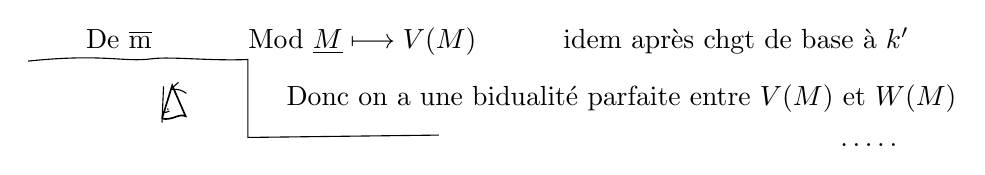
\begin{tikzpicture}[x=\linewidth,y=1cm]
\node[anchor=base west,inner sep=0pt] at (.06,1.18) {De $\overline{\mathrm{m}}$};
\node[anchor=base west,inner sep=0pt] at (.23,1.18) {\deleted{Mod} $\underline{M}\longmapsto V(M)$};
\node[anchor=base west,inner sep=0pt] at (.56,1.18) {idem après chgt de base à $k'$};
\draw (0,1.02) .. controls (.08,1.12) and (.10,1.00) .. (.13,1.05)
 .. controls (.15,1.08) and (.19,1.02) .. (.23,1.04)
 -- (.23,.05) -- (.43,.08);
\begin{scope}[shift={(.15,.45)},x=1cm,y=1cm]
 \draw[line width=.6pt] (-.12,-.16) -- (.01,.26) -- (.18,-.13)
  .. controls (.09,-.09) and (.01,-.19) .. (-.12,-.16);
 \draw (-.10,.25) -- (-.12,-.21) (.01,.23) -- (.09,.30);\draw (.01,.21) to[out=5,in=145] (.19,.16) (-.11,-.08) to[out=-5,in=210] (-.025,-.065);
 \fill (-.045,-.04) circle (.012);
\end{scope}
\node[anchor=base west,inner sep=0pt] at (.27,.46)
 {Donc on a une bidualité parfaite entre $V(M)$ et $W(M)$};
\node[anchor=base west,inner sep=0pt] at (.85,-.07) {.\,.\,.\,.\,.};
\end{tikzpicture}}

% @ 11
\[
 \underline{\operatorname{Aut}}_{\mathbb{O}}(M)\subset
 \underline{\operatorname{End}}_{\mathbb{O}}(M)
 \qquad\text{représentable si $M$ est proj., t f\hspace{.1em}\tikz[baseline=-.2ex,x=1ex,y=1ex]{\fill (0,.3) circle (.055);\fill (.12,.12) circle (.08);}}
\]

% @ 12
\noindent\hspace{.05\linewidth}\rule{.31\linewidth}{.4pt}

% @ 13
\[
 \mathord{\tikz[baseline=-.25ex,x=1ex,y=1ex]{\draw[line width=.08ex,line cap=round,line join=round] (.04,1.05) .. controls (.07,.4) and (.04,-.48) .. (.08,-.83) .. controls (.1,-.98) and (.15,-1.05) .. (.2,-1.12);\draw[line width=.09ex,line cap=round,line join=round] (.24,1.03)--(.28,1.15)--(.37,1.09) (.2,.56) .. controls (.16,.2) and (.21,-.57) .. (.32,-.89) (.19,.33) .. controls (.38,.31) and (.58,.53) .. (.66,.8) .. controls (.65,.37) and (.63,.19) .. (.96,.12);}}_n,\ D(\unsure{\vcenter{\hbox{\tikz[x=1ex,y=1ex]{\draw[line width=.12ex,line cap=round,line join=round] (0,0)--(.04,1.07)--(.94,1.09)--(.91,.6);\fill (.30,.82) circle[radius=.055ex];}}}|\Gamma|\Pi})\quad .\,.\,.
\]

% archive sheet number: 33

\cotefile{57}
\scanpage{3}
\uline{Local Picard schemes}.

Let $A$ be a complete local ring, \deleted{\unsure{Mr|Xx|X}} $S=\operatorname{Spec}(A)$, $U=S-\handwritten{\{}s\handwritten{\}}$ the complement of the closed point of $S$. We wish to interprete the Picard \deleted{gro} group $\operatorname{Pic}(U)$ as \deleted{som}e the group $P(k)$ of $k$-val\unsure{ae|ue}d points of a group-scheme $P$ defined over the residue field $k$ of $A$. Assume for simplicity that $U$ is regular, and that there exists a resolution of singularities for $S$ not changing $U$, i.e. a proper morphism
\[
f:X\handwritten{\longrightarrow}S
\]
inducing an isomorphism\deleted{\unsure{s}} $f^{-1}(U)\handwritten{\simeq}U$, such that $X$ be regular and equal to the closure of $f^{-1}(U)$ (this open set will be identified with $U$). Let $X_o$ be the special fiber of $X$, so that
\[
U=X-X_o\ .
\]
Because $X$ is regular, we have an exact sequence
\[
\begin{aligned}
\handwritten{(1)}\qquad\qquad & D\handwritten{\longrightarrow}\operatorname{Pic}(X)\handwritten{\longrightarrow}\operatorname{Pic}(U)\handwritten{\longrightarrow}0\ ,
\end{aligned}
\]
where $D$ is the group of divisors on $X$ concentrated on $X_o$ (which is a free group of finite type $\underline{Z}^{I}$, $I$ being the set of irreducible components of $X_o$). On the other hand, by the existence theorem for coherent sheaves, it is known that
\[
\begin{aligned}
\handwritten{(2)}\qquad\qquad & \operatorname{Pic}(X)\handwritten{\simeq}\underset{n}{\underset{\handwritten{\mathrel{\tikz[baseline=-.3ex,x=1em,y=1em]{\draw[line width=.45pt] (1,0)--(.08,.02) (.16,.10) .. controls (-.02,.05) and (-.02,-.12) .. (.17,-.17);}}}}{\lim}}\operatorname{Pic}(X_n)\ ,
\end{aligned}
\]
where $X_n=X\mathrm{x}_S S_n$, $S_n=\operatorname{Spec}(A/\underline{m}^{n+1})$. Assume we can find group schemes $P_n$ over $k$ and isomorphisms
\[
\begin{aligned}
\handwritten{(3)}\qquad\qquad & \operatorname{Pic}(X_n)\handwritten{\overset{\sim}{\mathrel{\tikz[baseline=-.3ex,x=1em,y=1em]{\draw[line width=.45pt] (0,0)--(1,0) (.88,.10)--(1,0)--(.98,-.19)--(.91,-.20);}}}}P_n(k)\ ,
\end{aligned}
\]
and transition morphisms $P_m\handwritten{\mathrel{\tikz[baseline=-.3ex,x=1em,y=1em]{\draw[line width=.45pt] (0,0)--(1,0)--(1,.12);}}}P_n$ $(m\handwritten{\geq}n)$ compatible with the transition morphisms for the $\operatorname{Pic}(X_n)$. Denoting by $P$ the pro-group $(P_n)$, or if one prefers, in case the transition morphisms $P_m\handwritten{\longrightarrow}P_n$ are affine, the inverse limit (EGA IV 8) of the $P_n$, we get a pro-group scheme resp. a group-scheme $P$, and an isomorphism
% archive sheet number: 2

\scanpage{4}
\[
\begin{aligned}
(4)\qquad\qquad & \operatorname{Pic}(X)\handwritten{\overset{\sim}{\mathrel{\tikz[baseline=-.3ex,x=1em,y=1em]{\draw[line width=.45pt] (0,0)--(.93,0);\draw[line width=.45pt] (.93,.05) .. controls (1.07,.10) and (1.08,-.14) .. (.96,-.12)--(.93,.05);}}}}P(k)\ .
\end{aligned}
\]
The map $D\handwritten{\longrightarrow}\operatorname{Pic}(X)\handwritten{\simeq}P(k)$ défines a morphism of (pro) \rlap{G}gro\uline{u}ps
\[
\begin{aligned}
(5)\qquad\qquad & D_k\handwritten{\longrightarrow}P\ ,
\end{aligned}
\]
where $D_k$ is the constant group-scheme with value $D$. Assuming that the cokernel of (5) exists in any reasonable sense a a pro-group scheme or a group-scheme, let $Q$ be this kernel. We get, in virtue of (1), an injective homomorphism
\[
\begin{aligned}
(6)\qquad\qquad & \operatorname{Pic}(U)\handwritten{\hookrightarrow}Q(k)\ ,
\end{aligned}
\]
the obstruction for an element of $\unsure{Q|\mathbb{Q}}(k)$ to be in the image being in $H^1(k,D'_k)$, where $D'_k$ is the image of $D_k$ in $P$ (it is again a constant group, with value a quotient $D'$ of $D$). \tikz[baseline=(s.base)]{\node[inner sep=1pt](s){\deleted{If}};\node[anchor=south west,inner sep=1pt](a) at ([xshift=-2pt,yshift=7pt]s.north west){\inserted{\handwritten{If $k$ is sep. closed, or if}}};\draw ([xshift=1pt,yshift=-2pt]s.north west) to[out=70,in=190] ([xshift=1pt,yshift=-2pt]a.south west)--([xshift=1pt,yshift=-2pt]a.south east) to[out=0,in=-90] ([xshift=3pt,yshift=5pt]a.south east);} $D'$ is torsion-free, for example is $D'$ is equal to $D$ i.e. (5) is injective, then this obstruction vanishes, and \deleted{$Q$ is a good candidat\unsure{e}} (6) is an isomorphism. Thus $Q$ looks a good candidate for a ``local Picard scheme''.

To construct the $P_n$'s, assume first that $A$ is a $k$-algebra, i.e. that a lifting of \tikz[baseline=(s.base)]{\node[inner sep=1pt](s){\deleted{\unsure{thh|the}}};\node[anchor=south,inner sep=1pt] at ([xshift=5pt,yshift=1pt]s.north){\inserted{the}};} residue field $k$ exists, and has been choosen. Then the natural candidate for $P_n$ (the only one I could think of, indeed !) would be
\[
\begin{aligned}
(7)\qquad\qquad & P_n=\underline{\operatorname{Pic}}_{X_n/k}\ .
\end{aligned}
\]
We know from Murre that the right had side is indeed representable by a scheme locally of finite type over $k$. There is however the usual trouble that we have indeed a canonical \uline{injective} morphism
\[
\begin{aligned}
(8)\qquad\qquad & \operatorname{Pic}(X_n)\handwritten{\hookrightarrow}P_n(k)\ ,
\end{aligned}
\]
but in general we are not sureit is bijective. However it is if $k$ is separably closed; more specifically, the obstruction for an element of $P_n(k)$ te be in the image of $\operatorname{Pic}(X_n)$ lies in the Brauer group \deleted{$\operatorname{Br}(k)$} \par\noindent\deleted{of $\unsure{Bo|B_o|k}\,\tikz[baseline=-.3ex,x=1em,y=1em]{\draw[line width=.6pt] (.10,.30) .. controls (-.04,.10) and (-.04,-.45) .. (.18,-.63);}$}
% archive sheet number: 3

\scanpage{5}
of the Artin ring $B_n=H^o(X_n,\underline{O}_{X_n})$. Assuming $U$ hence $X$ hence $X_n$ to be connected, this Artin ring is local, and it's Brauer group coincides with the Brauer group of its residue field $k_n$. Of course, \deleted{thus} for an element of $P(k)=\lim P_n(k)$, these vari\deleted{\unsure{e}}ous obstructions match together and come from an element of the Brauer group of the residue fi\rlap{l}e\rlap{e}ld $k'=\handwritten{\bigcap_n}k_n$ of the ring $H^o(X,\underline{O}_X)=\underset{\handwritten{n}}{\underset{\handwritten{\longleftarrow}}{\lim}}H^o(X_n,\underline{O}_{X_n})$, \deleted{of} which is just the normalisation of $A$. If for instance $A$ is \uline{normal}, \tikz[baseline=(s.base)]{\node[inner sep=1pt](s){$k'=k$};\node[anchor=south west,inner sep=1pt](a) at ([xshift=1pt,yshift=7pt]s.north west){\inserted{\handwritten{then}}};\draw ([xshift=-5pt,yshift=-3pt]s.south west) to[out=90,in=190] ([xshift=1pt,yshift=-2pt]a.south west)--([xshift=1pt,yshift=-2pt]a.south east) to[out=0,in=-90] ([xshift=3pt,yshift=4pt]a.south east);} and the obstruction lies in $\operatorname{Br}(k)$.

Whatever this be, defining $\unsure{Q|\mathbb{Q}}$ as before, we still do get an injective homomorphism (6), but even if (5) is injective, we cannot be sure that (6) is bijective. We are however if $k$ \unsure{is|ss} separable closed. Therefore, we still \deleted{get} can more or less describe $\mathord{\rlap{$\deleted{P}$}\handwritten{Q}}$ (or at least $\mathord{\rlap{$\deleted{P}$}\handwritten{Q}}(k)$) in termes of local Picard groups, in terms of \tikz[baseline=(s.base)]{\node[inner sep=1pt](s){descent};\node[anchor=south west,inner sep=1pt](a) at ([xshift=1pt,yshift=7pt]s.north west){\inserted{Galois}};\draw ([xshift=-5pt,yshift=-3pt]s.south west) to[out=90,in=190] ([xshift=1pt,yshift=-2pt]a.south west)--([xshift=1pt,yshift=-2pt]a.south east) to[out=0,in=-90] ([xshift=3pt,yshift=4pt]a.south east);} from the completion $A'$ of the strict henselization of $A$: if $U'=S'-\handwritten{\{}s'\handwritten{\}}$, where $S'=\operatorname{Spec}(A\mathord{\rlap{${}'$}(})$, \tikz[baseline=(s.base)]{\node[inner sep=0pt](s){and};\fill ([xshift=0pt,yshift=3pt]s.north) circle (.35pt);} if
\[
\begin{aligned}
(9)\qquad\qquad & \handwritten{\pi}=\operatorname{Gal}(\bar{k}/k)\ ,
\end{aligned}
\]
we will have an isomorphism
\[
\begin{aligned}
(10)\qquad\qquad & \deleted{\operatorname{Pic}}\unsure{\mathord{\rlap{$P$}Q}|\mathbb{Q}}(k)\handwritten{\simeq}\underline{\operatorname{Pic}}(U')^{\handwritten{\pi}}\ ,
\end{aligned}
\]
\deleted{This is perf provided $D'$ is torsion free, for instance (5)\,\tikz[baseline=-.3ex,x=1em,y=1em]{\fill (.12,-.35) circle (.35pt);\fill (.23,-.20) circle (.35pt);} injective\unsure{,|.}}

This is perfectly natural and in accordance with the familiar phenomena when dealing with \uline{global} Picard schemes. Therefore $Q$ looks like \rlap{a}the natural object to be called a \deleted{Picard} local Picard scheme.

To make sure it makes a sense, one will have however to analyze somewhat the inverse system $(P_n)$, and the morphism (5). Moreover, to feel really secure, one should check that up to canonical isomorphism, the group scheme $Q$ together with (10) does not depend on the choice of
% archive sheet number: 4

\scanpage{6}
t\rlap{e}h\rlap{h}e resolution; this \deleted{t}should not be hard whenever we have existence of resolutions in the strong sense of Hironaka, for instance in char.$0$ of if $\dim A=2$, \tikz[baseline=(s.base)]{\node[inner sep=1pt](s){I};\node[anchor=south west,inner sep=1pt](a) at ([xshift=-6em,yshift=7pt]s.north west){\inserted{\handwritten{so that two resolutions can be dominated by \unsure{-|a} third one.}}};\draw ([xshift=-4pt,yshift=-3pt]s.south west) to[out=90,in=190] ([xshift=1pt,yshift=-2pt]a.south west)--([xshift=1pt,yshift=-2pt]a.south east) to[out=0,in=-90] ([xshift=3pt,yshift=4pt]a.south east);} should point out that, in any case, the algebraic structure thus defined on $\operatorname{Pic}(U)$ depends in an essential way on the choice of the lifting of the residue field; an instructive example on which to study the dependance of this structure on the lifting is the one where $A$ is the completion of the local ring at the origin of the projecting cone of an elliptic curve (here $Q$ is isomorphic to the el liptic curve in question, for the \uline{given} lifting of $k$ ...).

I have to correct an inaccuracy that has slipped in, when defining $Q$ in the \unsure{wase|case} when $k$ is not separably closed, so as to get (10). One will then have to replace th\rlap{h}e constant group scheme $D_k$ by the twisted constant group scheme $\underline{D}$, deduced by descent from the constant group-scheme occuring after passage from $k$ to the separable closure. \figure{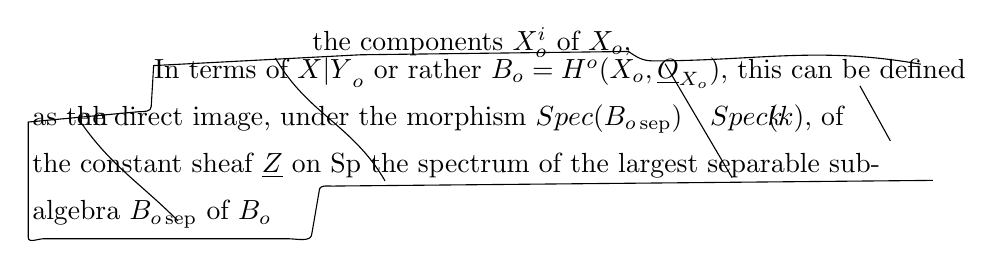
\begin{tikzpicture}[x=.44em,y=1.7em,every node/.style={anchor=base west,inner sep=0pt}]
\node at (10,0) {\deleted{In terms of \deleted{$\unsure{X|Y}_o$ or rather $B_o=H^o(X_o,\underline{O}_{X_o})$}, this can be defined}};
\node at (23,.60) {\deleted{\inserted{the components $X_o^i$ of $X_o$,}}};
\node at (0,-1) {\deleted{as t\rlap{e}h\rlap{h}e direct image, under the morphism $\operatorname{Spec}(B_{o\,\mathrm{sep}})\quad \operatorname{Spec}\mathord{\rlap{$k$}(}k)$, of}};
\node at (0,-2) {\deleted{the constant sheaf $\underline{Z}$ on \deleted{Sp} the spectrum of the largest separable sub-}};
\node at (0,-3) {\deleted{algebra $B_{o\,\mathrm{sep}}$ of $B_o$}};
\draw (73,.31) to[out=170,in=0] (51,.38) to[out=180,in=-35] (49,.58)--(27,.51)--(10,.28)--(9.8,-.59) to[out=-90,in=0] (8.8,-.70)--(-.3,-.92)--(-.3,-3.37) to[out=-90,in=180] (1,-3.40)--(21,-3.40) to[out=0,in=-90] (23,-3.28)--(23.6,-2.38) to[out=90,in=185] (25,-2.28)--(74,-2.16);
\draw (4,-.92) to[out=-55,in=135] (12,-3.02);
\draw (20,.44) to[out=-60,in=120] (29,-2.17);
\draw (52,.32)--(57.5,-2.10);
\draw (68,-.15)--(70.5,-1.32);
\end{tikzpicture}} This can be made explicit, in terms of the separable algebraic closures \deleted{of} $k_i$ of $k$ in the function fiel\tikz[baseline=(s.base)]{\node[inner sep=0pt](s){d};\fill ([xshift=-1pt,yshift=2pt]s.north west) circle (.3pt);}e of the irreducible components $X_o^i$ of $X_o$, as the \deleted{product of the schemes} direct image of the constant sheaf $\underline{Z}$ under the projection $\operatorname{Spec}(\handwritten{\prod}k_i)\handwritten{\longrightarrow}\operatorname{Spec}(k\unsure{)}$

To study the inverse system $(P_n)$, use the fact (SGA 6 XII) that the \deleted{\unsure{s}}transition morphisms are affine, which gives a sense to $P=\underset{\handwritten{\longleftarrow}}{\lim}P_n$ as an actual group-scheme. It's Lie algebra is the inverse limit of the Lie algebras \rlap{H}of the $P_n$, which are $H^1(X_n,\underline{O}_{X_n})$, therefore we get
% archive sheet number: 5

\scanpage{7}
\[
\begin{aligned}
(11)\qquad\qquad & \underline{\operatorname{Lie}}(P)\handwritten{\simeq}H^1(X,\underline{O}_X)\ .
\end{aligned}
\]
As $R^{\mathord{\rlap{$1$}\handwritten{\unsure{4|1}}}}f_{\handwritten{\unsure{*|k}}}(\underline{O}_X)$\unsure{;} is coherent and concentrated at the origin, it follows that its group of sections $H^1(X,\underline{O}_X)$ is of finite dimension. In fact, it seems, with a little care, that \deleted{\unsure{get|gei}} replacing if necessary $X$ by a \unsure{snitable|suitable} model \unsure{dmminating|dominating} it, we may assume that there exists an \tikz[baseline=(s.base)]{\node[inner sep=1pt](s){ideal};\node[anchor=south west,inner sep=1pt](a) at ([xshift=-4em,yshift=7pt]s.north west){\inserted{invertible}};\draw ([xshift=-4pt,yshift=-3pt]s.south west) to[out=90,in=-90] ([xshift=-4pt,yshift=-2pt]s.north west);\draw ([xshift=-3pt,yshift=5pt]a.south west) to[out=210,in=180] ([xshift=-4pt,yshift=-2pt]s.north west) to[out=0,in=180] ([xshift=1pt,yshift=-2pt]a.south east) to[out=0,in=-90] ([xshift=3pt,yshift=4pt]a.south east);} $J$ on $X$, \deleted{having} defining a subscheme $Z$ of $X$ having same support as $X_o$, and such that $\mathord{\tikz[baseline=(s.base)]{\node[inner sep=0pt](s){$J/J^2$};\node[anchor=south east,inner sep=1pt](a) at ([xshift=0pt,yshift=8pt]s.north west){$\inserted{\underline{L}=}$};\draw ([xshift=-4pt,yshift=-3pt]s.south west) to[out=90,in=0] ([xshift=-1pt,yshift=-2pt]a.south west) to[out=180,in=-90] ([xshift=-4pt,yshift=4pt]a.south west);\draw ([xshift=-4pt,yshift=-3pt]s.south west)--([xshift=9pt,yshift=16pt]s.north west);}}$ be an \uline{ample sheaf on} $Z$. This will imply that, replacing the system $(X_n)_{\handwritten{n}}$ by the system $(Z_n=V(J^{n+1}))_{\handwritten{n}}$, which defines \deleted{the} \deleted{\unsure{same}} an isomorphic pro-\rlap{\deleted{group}}\handwritten{object} of $\unsure{P|\mathbb{P}}$icard -schemes, we obtain an inverse system of group-schemes $P'_n=\underline{\operatorname{Pic}}_{Z_n/k}$ where for large $n$ the transition morphisms \deleted{are \unsure{h|b}} $P'_{n+1}\quad P'_n$ are \uline{isomorphisms} (because $H^1(Z_o,L^{\mathord{\tikz[baseline=(s.base)]{\node[inner sep=0pt](s){$\scriptstyle\mathrm{x}$};\draw[line width=.4pt] ([xshift=.7pt,yshift=1.2pt]s.center) ellipse[x radius=1.8pt,y radius=3.1pt];}}n})=H^2(Z_o,\underline{L}^{\mathord{\tikz[baseline=(s.base)]{\node[inner sep=0pt](s){$\scriptstyle\mathrm{x}$};\draw[line width=.4pt] ([xshift=.7pt,yshift=1.2pt]s.center) ellipse[x radius=1.8pt,y radius=3.1pt];}}n})=0$). \unsure{Thhs|Thus} it seems that, under the assumptions made \tikz[baseline=(s.base)]{\node[inner sep=1pt](s){,};\node[anchor=south west,inner sep=1pt](a) at ([xshift=-3em,yshift=9pt]s.north west){\inserted{\handwritten{from the start}}};\draw ([xshift=-2pt,yshift=-4pt]s.south west) to[out=90,in=180] ([xshift=1pt,yshift=-2pt]a.south east) to[out=0,in=-90] ([xshift=3pt,yshift=4pt]a.south east);} one can prove that the pro-group $(P_n)$ is essentially constant, hence its inverse limit $P$ is in fact a \uline{group scheme locally of finite type over} $k$. This is certainly so, at least, if $\dim A=2$, $A$ normal, as follows from the negative definiteness of the intersection matrix of the components of $X_o$.

\unsure{This|Thus|Thhs} $P$ seems to be definable in quite a reasonable way, and one still has to investigate the morphism (5) (or more accurately, \tikz[baseline=-.3ex,x=1em,y=1em]{\fill (.12,-.15) circle (.3pt);\fill (.24,0) circle (.3pt);} the morphisme $\underline{D}\handwritten{\longrightarrow}P$ defined by descent from the \rlap{x}case where $k$ is separably \tikz[baseline=(c.base)]{\node[anchor=base west,inner sep=0pt](c){closed;};\node[anchor=base west,inner sep=0pt](b) at ([xshift=.4em]c.base east){b\rlap{y}ut};\node[anchor=base west,inner sep=0pt](t) at ([xshift=.4em]b.base east){then};\node[anchor=base west,inner sep=0pt](w) at ([xshift=.8em]t.base east){we};\draw[gray,line width=.25pt] ([xshift=-1.8em,yshift=.8em]c.west)--([xshift=-.4em,yshift=-.8em]c.west) to[out=-5,in=185] ([yshift=-.6em]b.south) to[out=5,in=180] ([xshift=-.2em]t.west);\draw[line width=.35pt] ([xshift=-.2em,yshift=.1em]t.east) to[out=-60,in=165] ([xshift=-.1em,yshift=-.1em]w.west);} may as well assume $k$ separably closed \rlap{g}from the start\handwritten{,}\tikz[baseline=(s.base)]{\node[inner sep=1pt](s){.};\node[anchor=south west,inner sep=1pt](a) at ([xshift=-2em,yshift=7pt]s.north west){\inserted{\handwritten{which we will do}}};\draw ([xshift=-4pt,yshift=-3pt]s.south west) to[out=90,in=-90] ([xshift=-4pt,yshift=-2pt]s.north west);\draw ([xshift=-3pt,yshift=5pt]a.south west) to[out=210,in=180] ([xshift=-4pt,yshift=-2pt]s.north west) to[out=0,in=180] ([xshift=1pt,yshift=-2pt]a.south east) to[out=0,in=-90] ([xshift=3pt,yshift=4pt]a.south east);}). We would be particularly happy if this were a closed immersion, or what amounts to the same, if the morphism\deleted{\unsure{s|e}}
\[
\begin{aligned}
\handwritten{(12)}\qquad\qquad & D\mathrel{\tikz[baseline=-.3ex,x=1em,y=1em]{\draw[line width=.5pt] (0,0)--(1.5,0)--(1.32,.10) (1.5,0)--(1.32,-.13);\fill (1.22,-.15) circle (.35pt);}}\operatorname{NS}(X_o)
\end{aligned}
\]
is injective, were $\operatorname{NS}(X_o)=\underline{\operatorname{NS}}_{X_o\mathord{\tikz[baseline=-.25ex,x=1em,y=1em]{\draw[line width=.7pt] (0,-.05)--(.32,.72);\fill (.13,.45) ellipse[x radius=.06em,y radius=.08em];\fill (.14,.18) ellipse[x radius=.06em,y radius=.08em];}}k}(k)$, $\underline{\operatorname{NS}}=\underline{\operatorname{Pic}}/\underline{\operatorname{Pic}}^o$. (The equivalence comes from the fact that $P=\underline{\operatorname{Pic}}_{Z_n/k}$ for some \handwritten{l}arg\handwritten{e} $n$, and that $\deleted{\operatorname{Pic}}$
% archive sheet number: 6

\scanpage{8}
as recalled above\deleted{\unsure{x}}, the morphism $\underline{\operatorname{Pic}}_{Z_n\mathord{\tikz[baseline=-.25ex,x=1em,y=1em]{\draw[line width=.7pt] (0,-.05)--(.32,.72);\fill (.13,.45) ellipse[x radius=.06em,y radius=.08em];\fill (.14,.18) ellipse[x radius=.06em,y radius=.08em];}}k}\handwritten{\longrightarrow}\underline{\operatorname{Pic}}_{X_o/k}$ is affine, and hence $\operatorname{NS}(Z_n)\handwritten{\longrightarrow}\operatorname{NS}(X_o)$ has finite kernel.) I expect that this is always the case, \deleted{and it}\tikz[baseline=(s.base)]{\node[inner sep=0pt](s){xx};} In case $A$ is normal of dimension $2$, this follows from Du-Val - Mumford's negative definiteness. It would he nice to have a proof in general( perhaps through a negative definiteness of an intersection matric $X^i.C^j$, where for every irreducible component $X^i$ of $X_o$, $C^i$ denotes \tikz[baseline=(s.base)]{\node[inner sep=0pt](s){a curve};\node[anchor=south,inner sep=0pt] at ([xshift=-.6em,yshift=-1pt]s.north){\inserted{suitable}};} on $X^i$, for instance defined in terms of a suitable \deleted{ample} relatively ample sheaf on $X$ by taking intersections of corresponding hypersurface sections on the $X^i$'\deleted{\unsure{s}} ?).

In case (12) is indeed injective, we have no trouble defining
\[
\begin{aligned}
(13)\qquad\qquad & Q=P/\underline{D}
\end{aligned}
\]
as a \uline{group-scheme \rlap{r}l\rlap{e}ocally of finite type over} $k$. We then have
\[
\begin{aligned}
(14)\qquad\qquad & P^o\handwritten{\xrightarrow{\sim}}Q^o\ ,
\end{aligned}
\]
an isomorphism for the connected components, and
\[
\begin{aligned}
(15)\qquad\qquad & Q/Q^o=(P/P^o)/\underline{D}\handwritten{\simeq}\underline{\operatorname{NS}}_{Z_n/k}/\underline{D}\ ,
\end{aligned}
\]
where $n$ is chosen large enough. Of course (14) and (11) yield an i\rlap{x}somorphism
\[
\begin{aligned}
(16)\qquad\qquad & \underline{\operatorname{Lie}}(Q)\handwritten{\simeq}H^1(X,\underline{O}_X)\ .
\end{aligned}
\]
Let us remark by the way that we have an \uline{injective} restriction morphism
\[
\begin{aligned}
(17)\qquad\qquad & H^1(X,\underline{O}_X)\handwritten{\hookrightarrow}H^1(U,\underline{O}_U)=H_s^2(S)\qquad\qquad\mathord{\tikz[baseline=-.3ex,x=1em,y=1em]{\fill (.1,0) circle (.35pt);\fill (.3,.3) circle (.35pt);}}
\end{aligned}
\]
as one sees by remarking that, with the above notations for $\underline{J}$, $\underline{L}$, \inserted{\handwritten{the sheaf}} \deleted{\unsure{of}} $i_{\handwritten{*}}(\underline{O}_U)/\underline{O}_X$ $(i:U\handwritten{\longrightarrow}X$ the inclusion) has a composition series whose quotients are the $\underline{L}^{-n}$, $n\handwritten{\geq}1$, whose $H^o$ is zero, and the map (17) is just the canonical map $H^1(X,\underline{O}_X)\mathrel{\tikz[baseline=(s.base)]{\node[inner sep=0pt](s){$\unsure{\longrightarrow|\hookrightarrow}$};\path[fill=gray,opacity=.45] ([xshift=2pt,yshift=2pt]s.west)--([xshift=3pt,yshift=12pt]s.west)--([xshift=6pt,yshift=8pt]s.west)--([xshift=-1pt,yshift=2pt]s.east)--cycle;\draw[gray,line width=.6pt] ([xshift=4pt,yshift=11pt]s.west) to[out=250,in=100] ([xshift=3pt,yshift=5pt]s.west);}}H^1(X,i_{\handwritten{*}}(\underline{O}_U))$. Th\rlap{i}us, the Lie algebra of the local Picard scheme is identified with a subspace of $H^1(U,\underline{O}_U)$. (This suggests that if $A$ is Cohen-Macaulay of dim.$\handwritten{\geq 3}$, $Q$ is discrete, hence $\operatorname{Pic}(U)$ countable etc ).
% archive sheet number: 7

\scanpage{9}
The previous constructions rely heavily on the existence and choice of a field of representatives. Even this being granted, the question of caracterising $Q$ as an actual \uline{sche\`{m}e} \tikz[baseline=(s.base)]{\node[inner sep=0pt](s){,};\node[anchor=south west,inner sep=1pt](a) at ([xshift=-2em,yshift=7pt]s.north west){\inserted{over $k$}};\draw ([xshift=-3pt,yshift=-2pt]s.south west) to[out=90,in=180] ([xshift=0pt,yshift=-2pt]a.south west)--([xshift=0pt,yshift=-2pt]a.south east) to[out=0,in=-90] ([xshift=3pt,yshift=3pt]a.south east);} i.e. as a functor on the category of $k$-algebras, has not been touched. In fact, the description I can give of this functor is \tikz[baseline=(s.base)]{\node[inner sep=0pt](s){in};\node[anchor=south west,inner sep=1pt](a) at ([xshift=-3em,yshift=7pt]s.north west){\inserted{(tautological, and\deleted{)} is )}};\draw ([xshift=-3pt,yshift=-2pt]s.south west) to[out=90,in=180] ([xshift=0pt,yshift=-2pt]a.south west)--([xshift=0pt,yshift=-2pt]a.south east) to[out=0,in=-90] ([xshift=3pt,yshift=3pt]a.south east);} terms of a particular choice of a resolution $X$, and it really gives \deleted{rather} a description pf $P$ rather than $Q$. \deleted{To} One then still has to define $Q$ as the cokernel of the silly morphism $\underline{D}\handwritten{\longrightarrow}P$. As a matter of fact, even if we restrict to argument\unsure{s} $k'$ which are, say, finite extensions of $k$ (but not necessarily separabl\unsure{e} ones), I cannot describe $Q(k')$ in terms of local Picard groups of local rings as $A'=A\mathord{\tikz[baseline=(s.base)]{\node[inner sep=0pt](s){$\mathrm{x}$};\draw[line width=.5pt] ([xshift=.5pt,yshift=1.3pt]s.center) ellipse[x radius=3pt,y radius=4.5pt];}}_k k'$. The trouble, of course, is that $X\mathord{\tikz[baseline=(s.base)]{\node[inner sep=0pt](s){$\mathrm{x}$};\draw[line width=.5pt] ([xshift=.5pt,yshift=1.3pt]s.center) ellipse[x radius=3pt,y radius=4.5pt];}}_k k'$ will in general no longer be a resolution of $S'$, i.e. it will no longer be regular. However, such geometric descriptions will be possible provided we take as arguments algebras which are \tikz[baseline=(s.base)]{\node[inner sep=0pt](s){\deleted{smooth of formally}};\node[anchor=south west,inner sep=0pt] at ([yshift=2pt]s.north west){\inserted{\handwritten{geometrically regular}}};} \deleted{smooth} over $k$, so \deleted{taht} that tensoring with them will not destroy the regularity of $X$. (Thus, the case when $k'$ is a power series ring, for instance the completion of the local ring of $Q$ at the origin, $Q$ being smooth, is of interest ...) Let's now try to be specific. By definition \tikz[baseline=(s.base)]{\node[inner sep=0pt](s){for};\node[anchor=south west,inner sep=1pt](a) at ([xshift=-2em,yshift=7pt]s.north west){\inserted{\handwritten{more or less,}}};\draw ([xshift=-3pt,yshift=-2pt]s.south west) to[out=90,in=180] ([xshift=0pt,yshift=-2pt]a.south west)--([xshift=0pt,yshift=-2pt]a.south east) to[out=0,in=-90] ([xshift=3pt,yshift=3pt]a.south east);} any \tikz[baseline=(s.base)]{\node[inner sep=0pt](s){scheme};\node[anchor=south west,inner sep=1pt](a) at ([xshift=0em,yshift=7pt]s.north west){\inserted{\handwritten{affine}}};\draw ([xshift=-3pt,yshift=-2pt]s.south west) to[out=90,in=180] ([xshift=0pt,yshift=-2pt]a.south west)--([xshift=0pt,yshift=-2pt]a.south east) to[out=0,in=-90] ([xshift=3pt,yshift=3pt]a.south east);} $T$ over $k$, we have
\margin{\figure{\handwritten{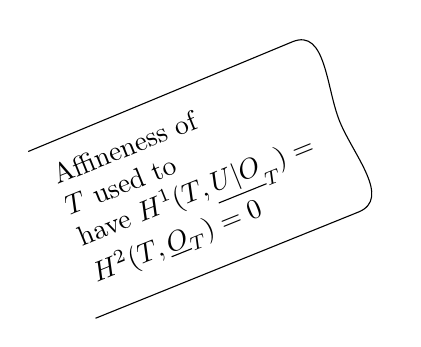
\begin{tikzpicture}[rotate=22,transform shape]
\node[inner sep=2pt,align=left](s){Affineness of\\$T$ used to\\have $H^1(T,\underline{\unsure{U|O}}_T)=$\\$H^2(T,\underline{O}_T)=0$};
\draw[line width=.4pt] ([xshift=-.3em,yshift=.6em]s.north west)--([xshift=.5em,yshift=.7em]s.north east) to[out=0,in=90] ([xshift=1em]s.east) to[out=-90,in=0] ([xshift=.4em,yshift=-.7em]s.south east)--([xshift=-.3em,yshift=-.7em]s.south west);
\end{tikzpicture}}}}
\[
\begin{aligned}
\handwritten{(18)}\qquad\qquad & P(T)=\underset{\handwritten{\longleftarrow}}{\lim}P_n(T)\handwritten{\hookleftarrow}\underset{\handwritten{n}}{\underset{\handwritten{\longleftarrow}}{\lim}}\operatorname{Pic}(X_{n_T}\deleted{\unsure{,\underline{O}_{X_{nT}}}})\handwritten{/\operatorname{Pic}\mathord{\tikz[baseline=(s.base)]{\node[inner sep=0pt](s){$(T)$};\fill ([xshift=-1pt,yshift=-5pt]s.south east) circle (.3pt);}}}\qquad (X_{n\,T}=X_n\mathord{\tikz[baseline=(s.base)]{\node[inner sep=0pt](s){$\mathrm{x}_{\unsure{\mathbb{k}|k}}$};\fill ([xshift=-.4em,yshift=-.25em]s.center) circle (.3pt);\fill ([xshift=-.5em,yshift=-.55em]s.center) circle (.3pt);}} T)\ .
\end{aligned}
\]
In fact, it is not hard to check that the left hand side functor is the étale sheaf (on $(\mathrm{Sch})_{/k}$): associated to the \deleted{left ha\unsure{n}} right-hand side functor. This comes from the more \tikz[baseline=(s.base)]{\node[inner sep=0pt](s){precise};\fill ([xshift=1pt,yshift=-2pt]s.south west) circle (.3pt);\fill ([xshift=3pt,yshift=-2pt]s.south west) circle (.3pt);} statement that the obstruction, for an element of $P(T)$, to come from an element of $\deleted{\operatorname{Pic}(X_{\unsure{nT|2T}})}\underset{\handwritten{n}}{\underset{\handwritten{\longleftarrow}}{\lim}}\operatorname{Pic}(X_{nT})$, lies in $H^2(T_{\text{ét}},\underline{G}_m)$ \handwritten{(} at least for $T$ affine, \deleted{\handwritten{(}}which is used to insure that it's $H^{\unsure{\rlap{$\scriptstyle1$}\handwritten{2}|\rlap{$\scriptstyle2$}\handwritten{1}}}$ and $H^{\unsure{\rlap{$\scriptstyle2$}\handwritten{3}|\rlap{$\scriptstyle3$}\handwritten{2}}}$ with values in $\underline{O}_T$ vanish\deleted{\handwritten{)}}, For simplicity, I have assumed here that $A$ is normal\handwritten{)}. As \tikz[baseline=(s.base)]{\node[inner sep=0pt](s){we};\draw[line width=.45pt] ([xshift=-.5em,yshift=.3em]s.south east) to[out=180,in=90] ([xshift=-.6em,yshift=-.08em]s.south east) to[out=-90,in=180] ([xshift=.4em,yshift=-.15em]s.south east);} have seen
% archive sheet number: 8

\scanpage{10}
on the other hand that $P$ is locally of finite presentation over $k$, it commutes (as afunctor) to \rlap{d}filtering direct limits of rings, and therefore it is known when we know it's restriction to arguments which are of finite type over $k$, and a fortiori \deleted{are} noetherian. For such \tikz[baseline=(s.base)]{\node[inner sep=0pt](s){arguments};\node[anchor=south west,inner sep=1pt](a) at ([xshift=-1em,yshift=7pt]s.north west){\inserted{\handwritten{(i.e. noetherian)}}};\draw ([xshift=-3pt,yshift=-2pt]s.south west) to[out=90,in=180] ([xshift=0pt,yshift=-2pt]a.south west)--([xshift=0pt,yshift=-2pt]a.south east) to[out=0,in=-90] ([xshift=3pt,yshift=3pt]a.south east);}, using the existence theorem for coherent sheaves, we can give a more geometric expression for the right hand side of (18), \deleted{namely}\tikz[baseline=(s.base)]{\node[inner sep=0pt](s){x};} Assume for simplicity $T=\operatorname{Spec}(B)$ affine, and let
\[
C=A\handwritten{\widehat{\mathord{\tikz[baseline=(s.base)]{\node[inner sep=0pt](s){$\mathrm{x}$};\draw[line width=.5pt] ([xshift=.5pt,yshift=1.3pt]s.center) ellipse[x radius=3pt,y radius=4.5pt];}}}}_k B=\lim A_n\mathord{\tikz[baseline=(s.base)]{\node[inner sep=0pt](s){$\mathrm{x}$};\draw[line width=.5pt] ([xshift=.5pt,yshift=1.3pt]s.center) ellipse[x radius=3pt,y radius=4.5pt];}}_k B\ ,
\]
which is an adic noetherian ring augmented to $B$ (the augmentation ideal being an ideal of definition). Consider $\deleted{\unsure{X_{TB}|X_T|Y_B|Y}}\mathord{\tikz[baseline=(s.base)]{\node[inner sep=0pt](s){$=$};\node[anchor=south west,inner sep=1pt](a) at ([xshift=-4em,yshift=7pt]s.north west){\inserted{\handwritten{$X\widehat{\otimes}_k B$}}};\draw ([xshift=-3pt,yshift=-2pt]s.south west) to[out=90,in=180] ([xshift=0pt,yshift=-2pt]a.south west)--([xshift=0pt,yshift=-2pt]a.south east) to[out=0,in=-90] ([xshift=3pt,yshift=3pt]a.south east);}}X\mathord{\tikz[baseline=(s.base)]{\node[inner sep=0pt](s){$\mathrm{x}$};\draw[line width=.5pt] ([xshift=.5pt,yshift=1.3pt]s.center) ellipse[x radius=3pt,y radius=4.5pt];}}_A C$, \tikz[baseline=(s.base)]{\node[inner sep=0pt](s){which};\node[anchor=south west,inner sep=0pt] at ([xshift=-1em,yshift=9pt]s.north west){\inserted{\deleted{$=X\widehat{\mathord{\tikz[baseline=(s.base)]{\node[inner sep=0pt](s){$\mathrm{x}$};\draw[line width=.5pt] ([xshift=.5pt,yshift=1.3pt]s.center) ellipse[x radius=3pt,y radius=4.5pt];}}}_k B$}}};} is a proper scheme over $C$. We then have
\[
\begin{aligned}
(19)\qquad\qquad & \operatorname{Pic}(X\handwritten{\widehat{\mathord{\tikz[baseline=(s.base)]{\node[inner sep=0pt](s){$\mathrm{x}$};\draw[line width=.5pt] ([xshift=.5pt,yshift=1.3pt]s.center) ellipse[x radius=3pt,y radius=4.5pt];}}}}_k B)\handwritten{\xrightarrow{\sim}}\underset{\handwritten{n}}{\underset{\handwritten{\longleftarrow}}{\lim}}\operatorname{Pic}(X_{nB}),\deleted{\unsure{\longrightarrow}P(B)}\handwritten{\operatorname{Pic}(X\widehat{\otimes}_{k}B)/\operatorname{Pic}(B)\hookrightarrow P(B)}
\end{aligned}
\]
and thus \rlap{P}on \uline{noetherian} arguments $B$, $P$ appears as the étale sheaf associated to the functor $B\handwritten{\mapsto}\operatorname{Pic}(X\handwritten{\widehat{\mathord{\tikz[baseline=(s.base)]{\node[inner sep=0pt](s){$\mathrm{x}$};\draw[line width=.5pt] ([xshift=.5pt,yshift=1.3pt]s.center) ellipse[x radius=3pt,y radius=4.5pt];}}}}_k B)\handwritten{/\operatorname{Pic}\unsure{(}B)}$ \tikz[baseline=(s.base)]{\node[inner sep=0pt](s){this};\node[anchor=south west,inner sep=1pt](a) at ([xshift=0em,yshift=7pt]s.north west){\inserted{\handwritten{which is a \uline{separated} presheaf,}}};\draw ([xshift=-3pt,yshift=-2pt]s.south west) to[out=90,in=180] ([xshift=0pt,yshift=-2pt]a.south west)--([xshift=0pt,yshift=-2pt]a.south east) to[out=0,in=-90] ([xshift=3pt,yshift=3pt]a.south east);} statement being complemented by the description given above of the group fcr obstructions for an element of $P(B)$ to \unsure{beleng|belang|belong} to $\operatorname{Pic}(X\handwritten{\widehat{\mathord{\tikz[baseline=(s.base)]{\node[inner sep=0pt](s){$\mathrm{x}$};\draw[line width=.5pt] ([xshift=.5pt,yshift=1.3pt]s.center) ellipse[x radius=3pt,y radius=4.5pt];}}}}_k B)$.

As for $\deleted{Q(B\unsure{)}}B\handwritten{\mapsto}Q(B)$, this appears as the \deleted{\unsure{sehaf|sheaf}} étale sheaf associated with the functor
\[
\begin{aligned}
(20)\qquad\qquad & B\handwritten{\longmapsto}\operatorname{Pic}(X\handwritten{\widehat{\mathord{\tikz[baseline=(s.base)]{\node[inner sep=0pt](s){$\mathrm{x}$};\draw[line width=.5pt] ([xshift=.5pt,yshift=1.3pt]s.center) ellipse[x radius=3pt,y radius=4.5pt];}}}}_k B)/\mathord{\tikz[baseline=(s.base)]{\node[inner sep=0pt](s){$\underline{D}$};\node[anchor=south west,inner sep=3pt](a) at ([xshift=-.2em,yshift=6pt]s.north west){\inserted{\handwritten{$(\operatorname{Pic}(B)+$}}};\draw[line width=.4pt] ([xshift=2pt,yshift=-2pt]a.south west) to[out=160,in=180] ([xshift=-2pt]a.west) to[out=90,in=180] (a.north) to[out=0,in=90] ([xshift=3pt]a.east) to[out=-90,in=0] ([xshift=-2pt,yshift=-2pt]a.south west);\draw ([xshift=-4pt,yshift=-5pt]s.south west) to[out=90,in=-140] ([xshift=-1pt,yshift=-2pt]a.south west);}}(B))\ (\handwritten{\mathrel{\tikz[baseline=(s.base)]{\node[inner sep=0pt](s){$\unsure{\hookrightarrow|\longleftrightarrow}$};\fill ([xshift=1pt,yshift=-5pt]s.south) circle (.3pt);}}}Q(B))\qquad\qquad\mathord{\tikz[x=1em,y=1em,baseline=-.8ex]{\fill (0,0) circle (.3pt);\fill (.13,.19) circle (.3pt);}}
\end{aligned}
\]
where $\underline{D}$ is the twisted constant group over $k$ defined above. For an element of $Q(B)$ to belong to the first hand side there are two successive obstructions, the first is in $H^1(\operatorname{Spec}(B),\underline{D})$, which vanishes \tikz[baseline=(s.base)]{\node[inner sep=0pt](s){if};\node[anchor=south west,inner sep=1pt](a) at ([xshift=-1em,yshift=7pt]s.north west){\inserted{\handwritten{for instance}}};\draw ([xshift=-3pt,yshift=-2pt]s.south west) to[out=90,in=180] ([xshift=0pt,yshift=-2pt]a.south west)--([xshift=0pt,yshift=-2pt]a.south east) to[out=0,in=-90] ([xshift=3pt,yshift=3pt]a.south east);} $\underline{D}$ is constant (for instance $k$ separably closed) and $B$ normal, the second is in the Brauer group of $B$, and vanishes \tikz[baseline=(s.base)]{\node[inner sep=0pt](s){if};\node[anchor=south west,inner sep=1pt](a) at ([xshift=-1em,yshift=7pt]s.north west){\inserted{\handwritten{for instance}}};\draw ([xshift=-3pt,yshift=-2pt]s.south west) to[out=90,in=180] ([xshift=0pt,yshift=-2pt]a.south west)--([xshift=0pt,yshift=-2pt]a.south east) to[out=0,in=-90] ([xshift=3pt,yshift=3pt]a.south east);} $X_o$ \unsure{hes|has} a zero-cycle of degree $1$.

Assume for simplicity that the irreducible components of $X_o$ are
% archive sheet number: 9

\scanpage{11}
geometricqlly irr\tikz[baseline=(s.base)]{\node[inner sep=0pt](s){e};\draw[line width=1pt] ([xshift=.2pt,yshift=-.5pt]s.north)--++(0,3pt);}ducible, i.e. $\underline{D}$ is constant, and assume $B$ geometrically regular over $k$. This second condition implies that $X\handwritten{\widehat{\mathord{\tikz[baseline=(s.base)]{\node[inner sep=0pt](s){$\mathrm{x}$};\draw[line width=.5pt] ([xshift=.5pt,yshift=1.3pt]s.center) ellipse[x radius=3pt,y radius=4.5pt];}}}}_k B$ is regular, and denoting by $U\handwritten{\widehat{\mathord{\tikz[baseline=(s.base)]{\node[inner sep=0pt](s){$\mathrm{x}$};\draw[line width=.5pt] ([xshift=.5pt,yshift=1.3pt]s.center) ellipse[x radius=3pt,y radius=4.5pt];}}}}_k B$ the inverse image of $U$ in this scheme, \deleted{the}\tikz[baseline=(s.base)]{\node[inner sep=0pt](s){x};}\deleted{first condition}\tikz[baseline=(s.base)]{\node[inner sep=0pt](s){x};}\deleted{\unsure{t|i}} this tog\rlap{t}e\rlap{e}ther with the first condition implies that \deleted{the} \tikz[baseline=(s.base)]{\node[inner sep=0pt](s){\deleted{\unsure{right}}};\node[anchor=south,inner sep=0pt] at ([yshift=3pt]s.north){\inserted{\deleted{left}}};}\deleted{ hand side of (20)}\tikz[baseline=(s.base)]{\node[inner sep=0pt](s){is};\node[anchor=south west,inner sep=1pt](a) at ([xshift=-4em,yshift=7pt]s.north west){\inserted{\handwritten{$\operatorname{Pic}(X\widehat{\otimes}_k B)/\underline{D}(B)$}}};\draw ([xshift=-3pt,yshift=-2pt]s.south west) to[out=90,in=180] ([xshift=0pt,yshift=-2pt]a.south west)--([xshift=0pt,yshift=-2pt]a.south east) to[out=0,in=-90] ([xshift=3pt,yshift=3pt]a.south east);} isomorphic to $\operatorname{Pic}(U\handwritten{\widehat{\mathord{\tikz[baseline=(s.base)]{\node[inner sep=0pt](s){$\mathrm{x}$};\draw[line width=.5pt] ([xshift=.5pt,yshift=1.3pt]s.center) ellipse[x radius=3pt,y radius=4.5pt];}}}}_k B)$. This shows that o n the sub-category of arguments $B$ which are \deleted{g\unsure{e}} noetherian and geometrically regular, $Q$ is the étale sheaf associated to the presheaf
\[
\begin{aligned}
(21)\qquad\qquad & B\handwritten{\longmapsto}\operatorname{Pic}(U\handwritten{\widehat{\mathord{\tikz[baseline=(s.base)]{\node[inner sep=0pt](s){$\mathrm{x}$};\draw[line width=.5pt] ([xshift=.5pt,yshift=1.3pt]s.center) ellipse[x radius=3pt,y radius=4.5pt];}}}}_k B)\handwritten{/\operatorname{Pic}(B)}\deleted{\unsure{(}}\handwritten{(\hookrightarrow}Q(B))\ .
\end{aligned}
\]
The obstruction for an element of $Q(B)$ to belong to $\operatorname{Pic}(U\handwritten{\widehat{\mathord{\tikz[baseline=(s.base)]{\node[inner sep=0pt](s){$\mathrm{x}$};\draw[line width=.5pt] ([xshift=.5pt,yshift=1.3pt]s.center) ellipse[x radius=3pt,y radius=4.5pt];}}}}_k B)$ \tikz[baseline=(s.base)]{\node[inner sep=0pt](s){is};\node[anchor=south west,inner sep=1pt](a) at ([xshift=-.5em,yshift=7pt]s.north west){\inserted{\handwritten{$/\operatorname{Pic}(B)$}}};\draw ([xshift=-3pt,yshift=-2pt]s.south west) to[out=90,in=180] ([xshift=0pt,yshift=-2pt]a.south west)--([xshift=0pt,yshift=-2pt]a.south east) to[out=0,in=-90] ([xshift=3pt,yshift=3pt]a.south east);} in the Brauer group $\operatorname{Br}(B)$. Thus, unde\rlap{e}r very stringent conditions on $B$ at least (being geometrically regular) we get a description of $Q(B)$ in terms of actual local Picard groups. I should have sta\rlap{e}ted that $U\handwritten{\widehat{\mathord{\tikz[baseline=(s.base)]{\node[inner sep=0pt](s){$\mathrm{x}$};\draw[line width=.5pt] ([xshift=.5pt,yshift=1.3pt]s.center) ellipse[x radius=3pt,y radius=4.5pt];}}}}_k B$ can also be interpreted as the inverse image of $U$ in the scheme $\unsure{\mathbb{S}|S}\mathrm{pec}(A\handwritten{\widehat{\mathord{\tikz[baseline=(s.base)]{\node[inner sep=0pt](s){$\mathrm{x}$};\draw[line width=.5pt] ([xshift=.5pt,yshift=1.3pt]s.center) ellipse[x radius=3pt,y radius=4.5pt];}}}}_k B)$, and thus makes a sense independently of the choice of a particular resolution.

One may wish to construct a local Picard scheme \deleted{without} also in case $A$ is not equi-caracteristic, which implies that $\mathrm{car}.k\handwritten{>}0$. It seems likely that this can be done if $k$ is perfect. The key-point here \deleted{seems} \deleted{to} is the construction of schemes $P_n$, which leads us to the foll\rlap{w}o\rlap{o}wing

\uline{\rlap{B}Problem}\quad Let $A$ be a local Artin ring with perfect residue field $k$ of car. $p\handwritten{>}0$, $X$ a proper scheme over $A$. Give a ``natural'' constructio\unsure{n} of a group scheme locally of finite type $P$ over $k$, together with an imbedding
\margin{\figure{\handwritten{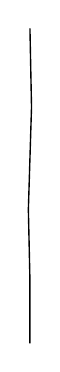
\begin{tikzpicture}\draw[line width=.5pt] (0,0)--(.02,-1)--(-.02,-2.3)--(0,-3.2)--(0,-4);\end{tikzpicture}}}}
\[
\begin{aligned}
(22)\qquad\qquad & \operatorname{Pic}(X)\handwritten{\hookrightarrow}P(k)\ ,
\end{aligned}
\]
the obstruction for an element of $P(k)$ to beling to $\operatorname{Pic}(X)$\handwritten{(}being in $\operatorname{Br}\ H^o(X,\underline{O}_X)$, and hence\handwritten{)}vanishing if $k$ is algebraically close\rlap{e}d.
% archive sheet number: 10

\scanpage{12}
Here is a candidate for a functor, which may t\unsure{\rlap{r}u\rlap{u}r|um|ur}n out to be representable, in which case this would be $P$. Let $\underline{A}$ be the ring-scheme over $k$ defined by $A$ (see Greenberg's papers, or Serre's in Bulletin Soc. Math.), so that
\[
\begin{aligned}
(23)\qquad\qquad & A\handwritten{\simeq}\underline{A}(k)\ .
\end{aligned}
\]
For every algebra $B$ over $k$, corsider the ring $\underline{A}(B)$, which is an algebra over $\underline{A}(k)=A$. We may thus consider
\[
X_B\overset{\mathrm{dfn}}{=}X\mathord{\tikz[baseline=(s.base)]{\node[inner sep=0pt](s){$\mathrm{x}$};\draw[line width=.5pt] ([xshift=.5pt,yshift=1.3pt]s.center) ellipse[x radius=3pt,y radius=4.5pt];}}_A\underline{A}(B)\ ,
\]
and consider the functor
\[
\begin{aligned}
(\rlap{3}24)\qquad\qquad & B\handwritten{\mathrel{\tikz[baseline=(s.base)]{\node[inner sep=0pt](s){$\longmapsto$};\draw[line width=.2pt,gray] ([xshift=-1pt,yshift=-1pt]s.east)--([xshift=-8pt,yshift=-22pt]s.west);}}}\operatorname{Pic}(X_B)\ .
\end{aligned}
\]
This of course may not be representable, even if $A=k$. However, it may turn out that the fppf sheaf associated to this functor is representable, and this then would give the looked for cand\deleted{\unsure{r}}idate for $P$. In any case, Artin's work gives us a very handy set of necessary and sufficie\unsure{n}% right edge cuts the last visible cell; no final t is visible
 conditions for a group functor to be representable by a scheme locally of finite type, and in principle it should be possible to decide wether or not the \deleted{functor} sheaf just considered satisfies to these conditions or not. If so, one may expect that the developments on local Picard schemes given for the case when there is a field of representatives will carry over to the case when the residue field \tikz[baseline=(s.base)]{\node[inner sep=0pt](s){is};\fill ([xshift=-1pt,yshift=5pt]s.north west) circle (.25pt);\fill ([xshift=.5pt,yshift=7pt]s.north west) circle (.25pt);} perfect with car.$\handwritten{>}0$.
% archive sheet number: 11

\scanpage{13}
In the construction of a local Picard scheme $Q$, we have seemed to u\rlap{n}se in a technically essential way the \tikz[baseline=(s.base)]{\node[inner sep=0pt](s){\deleted{fact}};\node[anchor=south west,inner sep=1pt](a) at ([xshift=-.5em,yshift=7pt]s.north west){\inserted{assumption}};} that $U$ is regular (plus resolution). I would conjecture that a reasonable \tikz[baseline=(s.base)]{\node[inner sep=0pt](s){loc al};\draw[line width=.3pt,gray] ([xshift=-1pt,yshift=-2pt]s.center) to[out=-10,in=200] ([xshift=6pt,yshift=1pt]s.center);} Picard scheme $Q$, \tikz[baseline=(s.base)]{\node[inner sep=0pt](s){can};\node[anchor=south west,inner sep=1pt](a) at ([xshift=-1em,yshift=7pt]s.north west){\inserted{locally of finite type over $k$,}};\draw ([xshift=-3pt,yshift=-2pt]s.south west) to[out=90,in=180] ([xshift=0pt,yshift=-2pt]a.south west)--([xshift=0pt,yshift=-2pt]a.south east) to[out=0,in=-90] ([xshift=3pt,yshift=3pt]a.south east);} be constructed also without this assumption (provided that a field of representatives is given, \rlap{l}or the residue field is perfect of char. $p\handwritten{>}0$, of course). Instead of a resolution of singularities, one \rlap{\deleted{p}}\handwritten{m}ay then wish to find a proper surjective morphism
\[
f:X\handwritten{\longrightarrow}S
\]
inducing an isomorphism $f^{-1}(U)\handwritten{\xrightarrow{\sim}}U$, and such that the corresponding map
\[
\operatorname{Pic}(X)\handwritten{\longrightarrow}\operatorname{Pic}(U)
\]
is \uline{surjective}. We then could repeat the construction of $P$, as $\lim\underline{\operatorname{Pic}}_{X_n/k}$, as above, and of $Q$ as $\operatorname{Coker}(\underline{D}\handwritten{\longrightarrow}P)$, where $\underline{D}$ is a group scheme corresponding to divisors concentrated on $X_o$ (possibly no longer discrete ?). Another way of approach would be to take a resolution of singularities $f:X\handwritten{\longrightarrow}S$, but where now we cannot assume any longer that $f^{-1}(U)\handwritten{\longrightarrow}U$ is an isomorphism, and to describ\rlap{x}e\deleted{\unsure{s}} a scheme $P$ in terms of invertible sheaves on $X$, together with \uline{descent data} of $\underline{L}\handwritten{|}f^{-1}(U)$ to $U$. A nice test for the yoga of local Picard schemes without regularity assumptions on $U$ would be to see if it is true in general that \rlap{f}\kern.2em or $A$ Cohen-Macaulay of dim $\handwritten{\geq3}$ (more generally, for $H^2_{\underline{m}}(A)=0$), the group $\operatorname{Pic}(U)$ is indeed countable, and for separably closed residue field \tikz[baseline=(s.base)]{\node[inner sep=0pt](s){\deleted{\unsure{invariant}}};\node[anchor=south west,inner sep=1pt](a) at ([xshift=0em,yshift=7pt]s.north west){\inserted{is invariant under}};} \uline{separable} field extension $k\handwritten{\longrightarrow}k'$, $A$ being replaced by $A\handwritten{\widehat{\mathord{\tikz[baseline=(s.base)]{\node[inner sep=0pt](s){$\mathrm{x}$};\draw[line width=.5pt] ([xshift=.5pt,yshift=1.3pt]s.center) ellipse[x radius=3pt,y radius=4.5pt];}}}}_k k'$ (which would express the expected \unsure{discrete|discreto} structure of the local Picard scheme).
% archive sheet number: 12

\cotefile{57}
\scanpage{20}
Dear Murre,\\

I am glad to hear that you are still willing to \rlap{\deleted{\unsure{make}}}gi\unsure{v}e the talk on unramified functors. Here what I can say to your questions.

1. The theorem about passage to quotient I alluded to is the foll\unsure{owing|hwing}:

\uline{Theorem} Let $f:X\handwritten{\to}Y$ be a morphisme of $S$-preschemes, assume either $X$ and $Y$ \tikz[baseline=(s.base)]{\node[inner sep=0pt](s){of};\node[anchor=south west,inner sep=1pt](a) at ([xshift=-.75em,yshift=6pt]s.north west){\inserted{locally}};\draw ([xshift=-3pt,yshift=-3pt]s.south west) to[out=100,in=180] ([xshift=0pt,yshift=-2pt]a.south west)--([xshift=0pt,yshift=-2pt]a.south east) to[out=0,in=-70] ([xshift=5pt,yshift=5pt]a.south east);} finite presentation over $\rlap{\deleted{$Y$}}\handwritten{S}$, or $Y$ loc noeth and $X$ \tikz[baseline=(s.base)]{\node[inner sep=0pt](s){of};\node[anchor=south west,inner sep=1pt](a) at ([xshift=-2em,yshift=6pt]s.north west){\inserted{locally}};} finite type over $Y\handwritten{\unsure{'}}$. Assume t\rlap{a}h\rlap{h}at the equivalence relation $\mathord{\tikz[baseline=(s.base)]{\node[inner sep=0pt](s){$X$};\node[anchor=south west,inner sep=1pt](a) at ([xshift=-1em,yshift=6pt]s.north west){\inserted{$R=$}};}}\mathbin{x}_{Y}X$ define\rlap{\deleted{e}}\handwritten{d} by $f$ is flat over $X$ i.e. $\mathrm{pr}_{1}:X\mathbin{x}_{Y}X\handwritten{\to}X$ is flat. Then the quotient $X/R$ exis\unsure{t}% clipped by right edge; no final s is visible
 in the strongest reasonable sense, \tikz[baseline=(s.base)]{\node[inner sep=0pt](s){i};\draw[line width=.6pt] ([xshift=-1.5pt,yshift=3pt]s.north)--([xshift=1.5pt,yshift=3pt]s.north) ([yshift=3pt]s.north)--([yshift=4.2pt]s.north);\fill ([yshift=-2pt]s.south) circle (.5pt);\draw[line width=.7pt] ([xshift=-1pt,yshift=-3.2pt]s.south)--([xshift=.4pt,yshift=-3.5pt]s.south);}.e. one can factor $f$ into a compositum $X\quad Z\quad Y$, with $\unsure{\mathbb{X}|\mathbb{Y}}\quad Z$ faithfully flat locally of finite presentation, $Z$ locally of finite \tikz[baseline=(s.base)]{\node[inner sep=0pt](s){\deleted{type}};\node[anchor=south west,inner sep=1pt](a) at ([xshift=0em,yshift=6pt]s.north west){\inserted{pres.}};} over $\mathord{\rlap{$Y$}\raisebox{-.15ex}{$S$}}$ (in fact of finite presentation over $S$ if $X$ is so) and $Z\handwritten{\mathrel{\tikz[baseline=(s.base)]{\node[inner sep=0pt](s){$\to$};\draw[gray,line width=.25pt] ([xshift=1pt,yshift=.5pt]s.west) to[out=30,in=180] ([xshift=5pt,yshift=2pt]s.west);}}}Y$ a monomorphism.

Of course the factorization is unique, andthe theorem can be expres-
sed by saying that the quotient sheaf (for the fpqc topology) $X/R$ is representable. T\tikz[baseline=(s.base)]{\node[inner sep=0pt](s){h};\draw[line width=.7pt] ([xshift=.2pt,yshift=2pt]s.south west) to[out=150,in=130] ([xshift=.6pt,yshift=-5pt]s.south west) to[out=70,in=140] ([xshift=-1pt,yshift=-2pt]s.south east)--([xshift=-.2pt,yshift=-5.5pt]s.south east); }at is in fact how the theorem is proved.

Raynaud has recently made a very nice (and non trivial) application of this theorem, by proving the following: if $S$ is the spectrum of a discrete valuation ring, $G$ a group prescheme of finite type over $\mathord{\tikz[baseline=(s.base)]{\node[inner sep=0pt](s){$S$};\fill ([xshift=1pt,yshift=-3pt]s.south) circle (.25pt);\fill ([xshift=-1pt,yshift=-5pt]s.south) circle (.22pt);}}$, $H$ a closed \tikz[baseline=(s.base)]{\node[inner sep=0pt](s){sub-group};\node[anchor=south west,inner sep=1pt](a) at ([xshift=-2em,yshift=6pt]s.north west){\inserted{and flat}};} scheme, such that $G_{t}/H_{t}$ is \deleted{affi} quasi-affine (where $t$ is the generic point of $S$) then $G/H$ is representable as a quasi-affine and flat $S$-scheme, which is even affine if $H$ is invariant (i.e. if $G$ is a flat group scheme of finite type with affine generic fibre, th\rlap{e}an $G$ is affine). This extends immediately to a b\kern-.2em\raisebox{-.6ex}{\inserted{\handwritten{\unsure{a}}}}\kern-.2em se which is regular of dim one. Raynaud is now trying to extend his construction to the c\rlap{q}ase when he drops the quasi-affinness assumption, namely to construct still $G/H$
% archive sheet number: 19

\scanpage{21}
as a quasi-projective scheme over $S$.

2. Theorem of the cube. I believe we discussed about it time ago, but maybe the proof I told you was valid only if one assumes the Pic functor of one of the \tikz[baseline=(s.base)]{\node[inner sep=0pt](s){\deleted{\unsure{functors}}};\node[anchor=south west,inner sep=1pt] at ([xshift=0em,yshift=6pt]s.north west){\inserted{factors}};} involved representable. To prove unramified-
ness of the functor \uline{Corr} however you need only a week infinit\rlap{i}es\rlap{i}emal form of the theorem of the square, for which you will find a proof in the manuscript notes I am joining on correspondance classes, containing also the proof\deleted{\unsure{s}} of the statements you were recalling in your question 4. I hope you will be able to read them, I agree the handwriting is wretched and the notes moreover very sketchy. - On the other hand, I recall you that the theorem of the cube follows rather formally once one knows separatedness of $\underline{\mathrm{Corr}}_{S}(X,Y)$ for two of the three factors involved, and using the usual formal properties of the Picard functor (among which commutation with inverse limits of Artin rings is the less trivial).

3. As for the separatedness of $\underline{\mathrm{Corr}}_{S}(X,Y)$, this is about trivial whene-
ver the Pic functor of one of the factors $X,Y$ is separated? Now this is \tikz[baseline=(s.base)]{\node[inner sep=0pt](s){certainly};\draw[gray,line width=.35pt] ([xshift=-3pt,yshift=2pt]s.south west)--([xshift=-2.4pt,yshift=-2pt]s.south west);\draw[line width=.55pt] ([xshift=-3pt,yshift=2pt]s.south west)--([xshift=-2.8pt,yshift=.5pt]s.south west);} the case \deleted{if} for $X$ if its geometric fibers are integral, (a fortiori if $X$ is an abelian scheme over $S$ !). To show this, one may assume $S$ the spectrum of a \tikz[baseline=(s.base)]{\node[inner sep=0pt](s){valuation};\node[anchor=south west,inner sep=1pt] at ([xshift=-1em,yshift=6pt]s.north west){\inserted{discrete}};} ring, and one is \rlap{d}reduced to show that if $\underline{L}$ is an invertible sheaf on $X$ whose restriction to \tikz[baseline=(s.base)]{\node[inner sep=0pt](s){the};\fill ([xshift=5pt,yshift=2pt]s.north east) circle (.3pt);\fill ([xshift=7pt,yshift=5pt]s.north east) circle (.3pt);} general fiber $X_{t}$ is trivial, then $\underline{L}$ is trivial. Now $X_{1}$ is an open subset of $X$, and the assumption on $\underline{L}$ can be expressed by saying that $\underline{\mathord{\rlap{$X$}L}}$ is defined by a Cartier divisor whose support is contained in the special fiber $X_{o}$. Now $X_{o}$ itself is already a Cartier divisor (d\rlap{i}efined by a global equation $\mathord{\rlap{$f$}t}=0$) and moreover is an integral subscheme of $X$, from this follows that the divisor $D$ is a multiple of $X_{o}$ (assume for
% archive sheet number: 20
